\documentclass[a4paper, 12pt]{article}
\usepackage[margin=2.5cm]{geometry}
%\usepackage{geometry}[2cm,2cm,2cm,2cm]
\usepackage[utf8]{inputenc}
\usepackage[nosumlimits]{amsmath}
\usepackage{amssymb,stmaryrd,amsthm,MnSymbol}
\usepackage{amsfonts,amssymb,amsopn}
\usepackage{mathrsfs}
 \usepackage[colorlinks=true,
            linkcolor=red,
            filecolor=red,
            citecolor=blue,
            urlcolor=blue,]{hyperref}
\usepackage[dvipsnames]{xcolor}
\usepackage{phoenician}

\usepackage{comment}
\usepackage{graphicx}
\usepackage{mathtools}
\usepackage{multicol}
\usepackage{tikz, tikz-cd}
\usetikzlibrary{arrows.meta, decorations.pathreplacing, calligraphy, positioning, calc}
\usepackage{adjustbox}

\usepackage{aligned-overset}
\usepackage{enumerate, enumitem}
\usepackage[ruled]{algorithm2e}
\usepackage{wrapfig}
\usepackage{placeins}

\usepackage{nicematrix}

\usepackage{caption, subcaption}
% for basis function plots
\newlength{\twosubht}
\newsavebox{\twosubbox}

\usepackage{natbib}
\let\OLDthebibliography\thebibliography
\renewcommand\thebibliography[1]{
  \OLDthebibliography{#1}
  \setlength{\parskip}{1pt}
  \setlength{\itemsep}{0pt plus 0.3ex}
}
\bibliographystyle{elsarticle-harv}

\usepackage{multirow}
\usepackage{booktabs}

%opening
\title{Adaptive Subdivision $k$-Form Spaces on the Matrix Level}
\author{Robert Piel\footnote{University of Surrey, School of Mathematics and Physics, UK (r.piel@surrey.ac.uk), ORCID: \url{https://orcid.org/0009-0001-8681-2493}} \ and
Werner Bauer\footnote{University of Surrey, School of Mathematics and Physics, UK (w.bauer@surrey.ac.uk), ORCID: \url{https://orcid.org/0000-0002-5040-4287}}
}


\newcommand{\todo}[1]{\vspace{5 mm}\par \noindent
	\framebox{\begin{minipage}[c]{0.95 \textwidth}
			\tt #1 \end{minipage}}\vspace{5 mm}\par}
\newcommand{\werner}[1]{{\color{magenta}WB says: #1}}
\newcommand{\robert}[1]{{\color{orange} #1}}
\usepackage[normalem]{ulem}  % \sout for struck-through deletions (normalem keeps \emph italic)
\newcommand{\ancestor}[1]{\big\lceil #1 \big\rceil_{\domseq}}     % coarsen a fine face to its covering active cell of \domseq
% Quadrisection operators. The superscript names the object being refined:
% a triangle for a face set, a star for a leaf star. Same stem, same slot,
% one glyph apart, so the two read as one family while staying distinguishable.
% The target level of the graded operator was a superscript "-> tau" and is now
% its third ARGUMENT: it is data the operator is applied to, not a choice of map,
% and Q^{star} is a single map rather than a family indexed by tau.
% Was: \mathcal{Q}^{f} and \mathcal{Q}^{\widehat{v} \to #2}. The latter put a
% \widehat{v} in the superscript, so the canonical call
% \quadriV{\targetlevel}(\domseq, \vertex{}{\coarseIdxtwo}) printed \widehat{v} twice
% in one expression; and "f" against "\widehat{v} \to \tau" was an unbalanced
% pairing of an object type against an equivalence class.
% Both operators now carry ONLY the operator symbol; their arguments are written
% out in the text as Q^{tri}(D, S) and Q^{star}(D, v, tau). Previously the
% domain sequence sat in a subscript, which made the stated signature
% \alldomseqs -> \alldomseqs untypeable (with both slots filled the expression is
% the *value*, not the map) and let the two sections drift into opposite
% conventions -- Sec. 3 wrote Q_D(faces) while the padding equations wrote
% Q_{faces}(D). Was: \mathcal{Q}^{\triangle}_{#1} and \mathcal{Q}^{\star \to #2}_{#1}.
\newcommand{\quadriF}{\mathcal{Q}^{\triangle}}                   % face quadrisection; args (domain sequence, level-indexed family of face sets)
\newcommand{\quadriV}{\mathcal{Q}^{\star}}                       % bare symbol; \quadriVup is built from it, and \tobecut call sites still typeset
% The target level rides on the OPERATOR, never in an argument slot. This is not
% the old \mathcal{Q}^{\star \to #2}_{#1} -- that carried source AND target and so
% named a value, not a map; here only the target ever appears, and the operator
% finds its own coarse end.
% RETIRED 2026-08-23: \quadriVat, the single-level vertex quadrisection acting on
% level #1. It was a special case of \quadriVup over one level, no step of the
% adaptive loop called it, and Remark~\ref{rem:graded_quadrisection_algorithm}
% now names \quadriF(., \FVleaf{#1}(v)) directly. Kept defined only so the
% \tobecut passages that still mention it typeset.
\newcommand{\quadriVat}[1]{\quadriV_{#1}}                        % acts on level #1
\newcommand{\quadriVup}[1]{\quadriV_{\rightarrow #1}}            % raises a vertex set to the target level #1
\newcommand{\lmin}{\l_{\min}}
\newcommand{\lminIdx}[1]{\l_{\min,#1}}
\newcommand{\lmax}{\l_{\max}}
\newcommand{\lmaxIdx}[1]{\l_{\max,#1}}
\newcommand{\levelSpan}[1]{s_{#1}}
% Level of the covering leaf face of a single face, i.e. where the ancestor walk
% of Corollary~\ref{cor:ancestor_walk} stops. Same slot as \lmin/\lmax, but a
% property of one FACE, not of a leaf star.
\newcommand{\lstar}{\l_{\ast}}
\newcommand{\sourcelevel}{\varsigma}                            % coarsest occupied level of a leaf star
\newcommand{\targetlevel}{\tau}                                 % marking target level
\newcommand{\Ltwoerror}{e_{L^2}}
\newcommand{\incl}[1]{{\color{red}#1}}
\newcommand{\checkit}[1]{{\color{red}#1}}
\newcommand{\RobertChanged}[1]{{\color{brown}#1}}
%\renewcommand{\checkit}[1]{{\color{red}#1}}
\newcommand{\tbd}[1]{{\color{red}#1}}
\newcommand{\highlight}[1]{{\color{cyan} #1}}
\newcommand{\needcite}{\highlight{(CITE)}} % flag a spot that likely needs a citation
% narrative guidance (draft scaffolding): lime-coloured text that reminds the
% reader/author how a piece fits the overall story. Concrete reader-facing
% guidance is used bare as \guidance{...}; not-yet-final refactoring reminders
% are wrapped as \todo{\guidance{...}}. Switch lime!70!black to lime for pure lime.
\newcommand{\guidance}[1]{{\color{lime!70!black} #1}}

% colors
\newcommand{\blue}{\color{blue}}
\newcommand{\red}{\color{red}}
\newcommand{\green}{\color{ForestGreen}}
\newcommand{\brickred}{\color{BrickRed}}

% highlighting
\newcommand{\hlcyan}[1]{{\sethlcolor{cyan}\hl{#1}}}
\newcommand{\hlorange}[1]{{\sethlcolor{orange}\hl{#1}}}

% handling simplices
\newcommand{\T}{\mathcal{T}}
\newcommand{\K}{\mathcal{K}}
\newcommand{\V}{\mathcal{V}}
\newcommand{\E}{\mathcal{E}}
\newcommand{\F}{\mathcal{F}}

\newcommand{\simplexname}{\sigma}
\newcommand{\simplex}[3]{\freeQ{\simplexname}{#1}{#2}{#3}}
\newcommand{\simplexnametwo}{\kappa}
\newcommand{\simplextwo}[3]{\freeQ{\simplexnametwo}{#1}{#2}{#3}}
\newcommand{\simplexsubset}[2]{\freeVec{\Delta}{#1}{#2}}

\newcommand{\vertex}[2]{\freeQ{v}{}{#1}{#2}}
% Vertex class: the orbit of one vertex under refinement, so it carries an
% IDENTITY index but NO level -- \vertex{\l}{#1} is its representative on level
% \l. This is the historical \widehat{v} notation (see the \quadriV comment
% above), reintroduced in Def.~\ref{def:vertex_class}. NOTE the decoration is
% shared with \reducedPatch = \widehat{\R}, which decorates a REGION; no vertex
% is ever reduced and no region is ever a class, so the two do not meet. If that
% ever bites, the fallback is bracket notation [\vertex{\l}{#1}].
\newcommand{\vertexClass}[1]{\widehat{v}_{#1}}
% Set of all vertex classes of the mesh hierarchy (Def.~\ref{def:vertex_class}).
% Hierarchy-level, NOT domain-sequence dependent: the orbits are taken under the
% injections of Eq.~\eqref{eq:vertex_injection}, which are read off T_l alone.
% Bijective with \V_\L(\T_\L), which is why properties are stated through the
% level-L representative. If Sec.~4 ends up needing only the classes that have a
% representative inside \domseq, that is a SUBSET and wants its own notation --
% \vertexClasses(\domseq[\L]) -- since a class born above \lzero need not meet
% any region.
\newcommand{\vertexClasses}{\widehat{\V}}
\newcommand{\vertexpos}[2]{\freeQ{\Vec{v}}{}{#1}{#2}}
\newcommand{\edge}[2]{\freeQ{e}{}{#1}{#2}}
\newcommand{\face}[2]{\freeQ{f}{}{#1}{#2}}
\newcommand{\barface}[2]{\overline{\face{#1}{#2}}}

% knob 1: raise the underbrace label toward the brace/equation (increase to pull closer)
\newlength{\ubraise}
\setlength{\ubraise}{2pt}
\newcommand{\ublabel}[1]{\smash{\raisebox{\ubraise}{$\scriptstyle #1$}}}

% knob 2: gap between the equation and the brace (default is 3pt; decrease to pull the brace up)
\newlength{\ubbracegap}
\setlength{\ubbracegap}{-2pt}
\makeatletter
\newcommand{\myunderbrace}[1]{%
  \mathop{\vtop{\m@th\ialign{##\crcr
      $\hfil\displaystyle{#1}\hfil$\crcr
      \noalign{\kern\ubbracegap\nointerlineskip}%
      \upbracefill\crcr\noalign{\kern3\p@}\crcr}}}\limits}
\makeatother

% adjacency relations
\newcommand{\KmKnl}[3]{\K^{#1}\K^{#2}_{#3}}
\newcommand{\VFl}[1]{\V\F_{#1}}
\newcommand{\EFl}[1]{\E\F_{#1}}
\newcommand{\FFl}[1]{\F\F_{#1}}
\newcommand{\VEl}[1]{\V\E_{#1}}
\newcommand{\EEl}[1]{\E\E_{#1}}
\newcommand{\FEl}[1]{\F\E_{#1}}
\newcommand{\VVl}[1]{\V\V_{#1}}
\newcommand{\EVl}[1]{\E\V_{#1}}
\newcommand{\FVl}[1]{\F\V_{#1}}

\newcommand{\KKltoL}[3]{\K^{#1}\K^{#1}_{#2 \to #3}}
\newcommand{\VVltoL}[2]{\V\V_{#1 \to #2}}
\newcommand{\EEltoL}[2]{\E\E_{#1 \to #2}}
\newcommand{\FFltoL}[2]{\F\F_{#1 \to #2}}

% indices for components
\newcommand{\coarseIdxone}{{\brickred i}}
\newcommand{\coarseIdxtwo}{{\brickred m}}
\newcommand{\fineIdxone}{{\brickred j}}
\newcommand{\fineIdxtwo}{{\brickred n}}

% indices for levels
\renewcommand{\l}{{\green\ell}}
\renewcommand{\L}{{\green L}}

\newcommand{\lzero}{{\green 0}}
\newcommand{\lone}{{\green {\l'}  }}
\newcommand{\ltwo}{{\green {\l''} }}
\newcommand{\lthree}{{\green {\l'''} }}

% numbers
\newcommand{\nc}{{\color{Magenta} n_c}}
\newcommand{\nr}{{\color{Magenta} n_r}}
\newcommand{\ns}{{\color{Magenta} n_s}}

% refinement stencils
\newcommand{\RSt}{\mathrm{R}}
\newcommand{\cRSt}{\RSt_{c}}
\newcommand{\R}{\mathcal{R}}
\newcommand{\Sreg}{\mathcal{S}}                             % a second region, used for the ancestor

% derivative stencil
\newcommand{\DSt}{\mathrm{D}}

% macros that determine the general format
% constrained quantity
\newcommand{\constrQ}[5]{ ( {#1}^{#2}_{#3 \vert #4} )_{#5}} % e.g. \constr_vec{c}{k}{\ell}{L}{i} renders as (c^k_{l|L})_i
% constrained vector (no index i)
\newcommand{\constrVec}[4]{ {#1}^{#2}_{#3 \vert #4} }
% free quantity
\newcommand{\freeQ}[4]{ ( {#1}^{#2}_{#3} )_{#4}}
% free vector (no index i)
\newcommand{\freeVec}[3]{ {#1}^{#2}_{#3}}

% subdiv operators
\newcommand{\Sop}[3]{\mathcal{S}^{#1}_{{#2} \to {#3}}}
\newcommand{\Smat}[3]{\mathbf{\mathrm{S}}^{#1}_{#2 \to #3}}
\newcommand{\Smatij}[5]{\left(\mathbf{\mathrm{S}}^{#1}_{#2 \to #3}\right)_{#4 #5}}

% accumulated subdiv matrix
% DIRECTION CONVENTION: the arrow points from coarse to fine, ALWAYS.
% \Aop{k}{\l}{\l'} is the accumulated subdivision operator on k-forms; the
% topological form \Aop{}{\l}{\l'} with \l < \l' is quadrisection, taking a face
% (set) to its descendants on the finer level. The coarsening direction is NOT
% written by reversing this arrow -- it is \anc{\l}, see the face ancestor
% operator below. This used to be an overload on \Aop and was split out because
% \Aop already carried two meanings (k-forms vs. faces) before the direction
% added a third.
\newcommand{\Aop}[3]{\mathcal{A}^{#1}_{{#2} \to {#3}}}
\newcommand{\Amat}[3]{\mathbf{\mathrm{A}}^{#1}_{#2 \to #3}}
\newcommand{\Amatij}[5]{\left(\mathbf{\mathrm{A}}^{#1}_{#2 \to #3}\right)_{#4 #5}}

\newcommand{\primalAop}[4]{ {\mathcal{A}^{#1}_{{#2} \to {#3}|{#4} }}  }
\newcommand{\dualAop}[4]{ {\mathcal{B}^{#1}_{{#2}|\,{#3} \rightarrow {#4}} }}

% Whit and Loop, and their Aops
\newcommand{\Whit}{\mathrm{Whit}}
\newcommand{\Loop}{\mathrm{Loop}}
\newcommand{\AopWhit}[2]{\Aop{\Whit}{#1}{#2}}
\newcommand{\AopLoop}[2]{\Aop{\Loop}{#1}{#2}}

% derivative
\newcommand{\extd}{\mathbf{d}}
\newcommand{\auxextd}{\overset{\sim}{\vphantom{a}\smash{\mathbf{d}}}} % auxiliary derivative
\newcommand{\Dmat}[2]{\mathbf{D}^{#1}_{#2}} % derivative matrix
\newcommand{\Dmatij}[4]{\big(\mathbf{D}^{#1}_{#2}\big)_{#3 #4}} % derivative matrix with components

\newcommand{\dd}{\mathrm{d}_d} % discrete exterior derivative
\newcommand{\ddk}[1]{\mathrm{d}_d^{#1}}
\newcommand{\ddkl}[2]{\mathrm{d}_{d,#2}^{#1}}

% FEEC spaces
\newcommand{\FEECspace}[2]{\Lambda^{#1}_{#2}}
\newcommand{\FEECbasis}{\psi}
\newcommand{\FEECbases}{\Psi}
\newcommand{\FEECspaceZero}[2]{\mathring{\Lambda}^{#1}_{#2}}

% subdiv spaces
\newcommand{\SDFspace}[3]{\mathcal{S}\Lambda^{#1}_{#2 \vert #3}}
\newcommand{\SDFbasis}{\phi}
\newcommand{\SDFbases}{\Phi}
\newcommand{\SDFbasesZero}{\mathring{\SDFbases}}
\newcommand{\SDFspaceZero}[3]{\mathring{\mathcal{S}}\Lambda^{#1}_{#2 \vert #3}}

% operators for BCs
\newcommand{\trace}{\mathrm{tr}}
\newcommand{\Vint}{\mathring{\V}}
\newcommand{\Eint}{\mathring{\E}}
\newcommand{\Fint}{\mathring{\F}}
\newcommand{\Kint}{\mathring{\K}^k}
\newcommand{\BCAop}[3]{\mathring{\mathcal{A}} {}^{#1}_{#2 \to #3}}
\newcommand{\BCAmat}[3]{\mathring{\mathrm{A}} {}^{#1}_{#2 \to #3}}
\newcommand{\BCBEop}[4]{\mathring{\mathcal{B}} {}^{#1}_{#2 \vert #3 \to #4}}

% hierarchical spaces
\newcommand{\I}{\mathcal{I}}
\newcommand{\II}{\mathbb{I}}
\newcommand{\heth}{\textphnc{H}}
\newcommand{\allcoverings}{\mathscr{C}}
\newcommand{\allpartitions}{\mathscr{C}^{\mathrm{sp}}}

\newcommand{\activeDoFs}{\mathbb{A}}
\newcommand{\inactiveDoFs}{\mathbb{I}}
\newcommand{\D}{\activeDoFs}
\newcommand{\activeDoFSet}[2]{\activeDoFs^{#1}_{#2}}
\newcommand{\activeDoFSetZero}[2]{\mathring{\activeDoFs}{}^{#1}_{#2}}
\newcommand{\activeSDFspaces}[2]{\mathcal{S}\activeDoFSet{#1}{#2}}

% The embedding level is absorbed into the domain sequence: #3 is set as a SUBSCRIPT on
% #2 rather than after a \vert, so \hierSDFspace{k}{\domseq}{\L} gives \mathcal{S}\mathbb{A}^k_{\mathcal{D}_\L}.
% Legitimate for the reason recorded in Definition~\ref{def:domseq}: trailing empty regions
% let the single index \L carry both the selection depth and the representation mesh.
% Pass an EMPTY #3 when the level already sits inside #2, as at eq:quadrisection_monotone,
% where #2 is an operator application and the level belongs on its argument.
% Robust because both macros appear inside \caption.
\makeatletter
\DeclareRobustCommand{\hierSDFspace}[3]{\mathcal{S}\activeDoFs^{#1}_{#2\ifx\@empty#3\@empty\else_{#3}\fi}}
\DeclareRobustCommand{\hierSDFspaceZero}[3]{\mathring{\mathcal{S}}\activeDoFs^{#1}_{#2\ifx\@empty#3\@empty\else_{#3}\fi}}
\makeatother
\newcommand{\inactiveSDFspace}[3]{\mathcal{S}\inactiveDoFs^{#1}_{#2 \vert #3}}
\newcommand{\coarseInactiveSDFspace}[3]{\mathcal{S}\inactiveDoFs^{#1, \mathrm{c}}_{#2 \vert #3}}
\newcommand{\fineInactiveSDFspace}[3]{\mathcal{S}\inactiveDoFs^{#1, \mathrm{f}}_{#2 \vert #3}}

% general maths
\renewcommand{\powerset}{\mathbb{P}}
\newcommand{\inclusion}{\iota}
\newcommand{\auxincl}{\overset{\sim}{\vphantom{a}\smash{\iota}}} % auxiliary derivative
\newcommand{\support}{\mathrm{supp}}
\newcommand{\pfrac}[2]{\frac{\partial #1}{\partial #2}}
\newcommand{\M}{\mathcal{M}}
\newcommand{\vvert}[1]{\left\vert #1 \right\vert}
\newcommand{\dimlk}[2]{\big\vert \K^{#2}_{#1} \big\vert}
\newcommand{\sumdimlk}[2]{\vert \K^{#2}_{#1} \vert}
\newcommand{\closure}[1]{\overset{\circ}{#1} {}}
\renewcommand{\complement}{\mathsf{c}}

% widecheck and widehat
\DeclareFontFamily{U}{mathx}{}
\DeclareFontShape{U}{mathx}{m}{n}{<-> mathx10}{}
\DeclareSymbolFont{mathx}{U}{mathx}{m}{n}
\DeclareMathAccent{\widehat}{0}{mathx}{"70}

% A *fixed-size* \widecheck, so the accent no longer grows with the width of the
% letter it sits on. The mathx glyph "71 carries a nextlarger chain, which is what
% made \widecheck{\M} much wider than \widecheck{\R}. Instead we take the ordinary
% \check glyph (OT1 slot 20 of cmr) from a copy of cmr loaded at a magnified size,
% and declare a real math accent on it, so that height and skew handling and
% shrinking in script styles all keep working at one constant width. Adjust the
% 1.4 below to taste (1.0 gives exactly \check).
\DeclareFontFamily{OT1}{wcheck}{}
\DeclareFontShape{OT1}{wcheck}{m}{n}{<->s*[1.4] cmr10}{}
\DeclareSymbolFont{wcheck}{OT1}{wcheck}{m}{n}
\DeclareMathAccent{\widecheck}{0}{wcheck}{20}

% macros for specific spaces
\newcommand{\CG}{\mathrm{CG}}
\newcommand{\NED}{\mathrm{NED}}
\newcommand{\DG}{\mathrm{DG}}
\newcommand{\Hcurl}{H(\text{curl})}
\newcommand{\HcurlM}[1]{H\left(\text{curl}, #1\right)}
\newcommand{\HocurlM}[1]{\mathring{H}\left(\text{curl}, #1\right)}

%%% to be removed %%%
\newcommand{\rmA}{A}

%% maths environments
\newtheorem{theorem}{Theorem}[section]
\newtheorem{definition}[theorem]{Definition}
\newtheorem{lemma}[theorem]{Lemma}
\newtheorem{proposition}[theorem]{Proposition}
\newtheorem{corollary}[theorem]{Corollary}
\newtheorem{example}[theorem]{Example}
\newtheorem{remark}[theorem]{Remark}
\newtheorem{assumption}[theorem]{Assumption}
\newtheorem{numberedproof}[theorem]{Proof}
\newtheorem{problem}[theorem]{Problem}
\newtheorem{conjecture}[theorem]{Conjecture}


%% adjust equation numbering to IMA style
\numberwithin{equation}{section}
\numberwithin{algocf}{section}

% =========================================================================
% Migration to domain sequences (2026-08-11).
%
% Macros ported verbatim from adaptive_theory_paper/main.tex so that the
% imported definitions render identically in both papers. Line numbers below
% refer to that file.
% =========================================================================

% --- annotation macros (adaptive_theory:68, :85) ---
\newcommand{\prose}[1]{{\color{magenta} #1}}   % connective text written here, not imported
\newcommand{\tobecut}[1]{{\color{red} #1}}     % cut candidate; plain colour so it may span paragraphs

% --- domain sequences and patch operators (adaptive_theory:88--95, :344) ---
\newcommand{\extendedPatch}[1]{\widecheck{#1}}
\newcommand{\ancestorPatch}[1]{\left\lceil #1 \right\rceil}
\newcommand{\reducedPatch}[1]{\widehat{#1}}
% \domseq takes the level as an OPTIONAL argument: \domseq is \mathcal{D}, \domseq[\L]
% is \mathcal{D}_\L. Robust (\DeclareRobustCommand) because it appears inside \caption.
\makeatletter
\DeclareRobustCommand{\domseq}[1][]{\mathcal{D}\ifx\@empty#1\@empty\else_{#1}\fi}
\makeatother
\newcommand{\alldomseqs}{\mathscr{D}}
% NOT ported: \domseql / \coveringl. notation/glossary.md records an unresolved
% subscript-order collision (those two are target-first, \SDFspace / \recSpace /
% \hierBasis / \intermediateSpace are level-first) whose fix is diagnosed but
% unapplied. This paper has no use for the two-index form, so it does not inherit it.

% --- regions and their boundaries (adaptive_theory:102--103, :818) ---
\newcommand{\boundary}{\partial}                            % full boundary of a region

% --- region DoF sets (adaptive_theory:103, :341--342, :347, :365, :376, :956) ---
\newcommand{\patchDoFs}[2]{{#1}{}^{#2}}
\newcommand{\openPatchDoFs}[2]{\mathring{#1}{}^{#2}}
\newcommand{\intermediateSpace}[3]{X^{#1}_{#2,#3}}
\newcommand{\intermediateDoFs}[3]{\mathbb{X}^{#1}_{#2,#3}}
\newcommand{\inactiveDoFSet}[2]{\inactiveDoFs^{#1}_{#2}}

% --- admissibility predicates (adaptive_theory:1819, :1810) ---
\newcommand{\refFan}[1]{\Theta_{#1}}                        % refinement fan of a vertex
\newcommand{\birthLevel}{b}
\newcommand{\leafF}[1]{\F^{\mathrm{leaf}}_{#1}}             % leaf (uncovered) faces on a level
\newcommand{\leafMesh}{\F^{\mathrm{leaf}}}                  % leaf mesh: the leaf faces of all levels together
% The two ways UP the hierarchy, deliberately parallel in notation and defined
% back to back at the head of Section~\ref{subsec:vertex_neighbourhoods}
% (Def.~\ref{def:face_ancestor} and Def.~\ref{def:covering_face}), because the
% star ancestry and the leaf star are the images of one mesh star under them:
%   \anc{\l'}(.)      -- to the ancestor on the prescribed level \l'. Read off
%                        the uniform meshes alone, so no domain-sequence input.
%   \coveringFace(.)  -- to the covering LEAF face, whose level is whatever the
%                        domain sequence makes it. Domain-sequence dependent.
% Both apply facewise to a set of faces. The subscript slot of \anc is the LEVEL
% the result is read at, matching \leafF, \FVl, \FVleaf and \FVanc.
% \anc extends \ancestorPatch rather than duplicating it: the two agree on
% quadrisection-closed regions, but \anc is defined on arbitrary face sets,
% which is what the star ancestry of a mesh star needs.
% \coveringFace was \mathrm{leaf}; renamed to \mathrm{cov} so that the pair
% anc/cov both name the RELATION to the argument rather than the type of answer.
\newcommand{\anc}[1]{\mathrm{anc}_{#1}}                     % face ancestor on level #1
\newcommand{\coveringFace}{\mathrm{cov}}                    % leaf face covering a given face
% Leaf star of a vertex. The ARGUMENT is a LEVEL SLICE, not a read level:
% \FVleaf{} is the whole leaf star (Def. leaf_star, read at level L) and
% \FVleaf{#1} is its level-#1 slice, i.e. the leaf faces it carries at level #1. Same slot as \FVl and \leafF, and \FVleaf{\l} \cap \F_\l is
% \FVl{\l} \cap \leafF{\l}. The marker rides at the END of the compound, so \FV
% stays one atomic symbol; \F^{leaf}\V would wedge the superscript between the
% two letters and read as a product.
% Was \St = \mathrm{St}: the companion paper uses St for the mesh star SPACE of
% a vertex, and this is a set of faces.
\newcommand{\FVleaf}[1]{\F\V^{\mathrm{leaf}}_{#1}}          % leaf star of a vertex at level #1
% Star ancestry: same argument slot as \FVl and \FVleaf, i.e. #1 is the LEVEL at
% which the set of faces is read. Unlike the leaf star it is read off the uniform
% meshes alone and carries no dependence on a domain sequence, which is what makes
% the graded vertex quadrisection add a fixed set, see
% Lemma~\ref{lemma:graded_quadrisection_closed_form}. Not expressible through
% \ancestorPatch, which Definition~\ref{def:domseq} only supplies on
% quadrisection-closed sets, and a mesh star is not one -- this is exactly the
% gap \anc fills, and \FVanc{\l'}(v) is now literally \anc{\l'} of the mesh star.
\newcommand{\FVanc}[1]{\F\V^{\mathrm{anc}}_{#1}}            % star ancestry of a vertex at level #1

% --- the admissible class, re-based on domain sequences (adaptive_theory:270--272).
% \allcoverings and \allpartitions previously read \mathscr{C} and \mathscr{C}^{sp};
% they name the same two sets, now indexed by domain sequences rather than coverings,
% so they are redefined rather than duplicated.
\renewcommand{\allcoverings}{\mathscr{D}}
\renewcommand{\allpartitions}{\mathscr{D}^{\mathrm{ad}}}
\newcommand{\allpartitionsStar}{\mathscr{D}^{\mathrm{ad}\ast}}

% The symbol formerly written \string\C (originally \heth, a covering) has been retired
% in favour of \domseq, defined above. The note that stood here claimed \string\C and
% \domseq[\L] "render identically as \mathcal{D}_\L". That was never true, since the old
% \string\C carried no subscript at all. All 227 of its occurrences were swept to \domseq.
% \string\C is now deliberately left UNDEFINED, so that any missed occurrence fails loudly
% at compile time rather than silently rendering the right glyph.

\begin{document}

\maketitle

\vspace{-2.0em}

\begin{abstract}
We provide the algorithmic and computational complement to the theoretical framework of~\guidance{\cite{companion_paper}} for hierarchical subdivision $k$-form spaces on triangular meshes. The central observation is that every basis function is represented by a column of the accumulated subdivision matrix. Selecting active degrees of freedom results in collecting their corresponding columns into the hierarchical subdivision matrix. This sparse matrix reduces all downstream operations like matrix assembly or residual evaluation to standard sparse linear algebra on the finest mesh $\T_\L$ without recomputing any integrals. The substantive question is which selections of active degrees of freedom are admissible, in particular linearly independent and exactness of the complex. We answer this question via purely combinatorial admissibility conditions. We provide explicit algorithms for constructing the active degrees of freedom from a domain sequence, obtained level by level by adding fine degrees of freedom and removing linearly dependent coarse ones.

For the adaptive solution of PDEs, we describe a \textsc{Solve}--\textsc{Estimate}--\textsc{Mark}--\textsc{Refine}--\textsc{Pad} loop in which the non-standard \textsc{Pad} step enforces the admissible domain sequence conditions after Dörfler marking by applying pinch resolution, \checkit{confinement padding}, and grading, refining the coarse regions that would otherwise break admissibility. Numerical experiments on the Maxwell eigenvalue problem confirm that exact admissible domain sequences reproduce the reference spectrum without spurious modes and adaptive experiments on the mixed vector Laplace equation demonstrate the adaptive loop.
\end{abstract}

\tableofcontents

\section{Introduction}

The finite element exterior calculus (FEEC)~\cite{Arnold.FEEC} provides a systematic framework for constructing stable, structure-preserving discretisations of partial differential equations (PDEs) involving differential forms. Its central structure is the discrete de Rham complex: a sequence of finite-dimensional function spaces connected by the exterior derivative $\extd$. Exactness of this complex is the key algebraic property that prevents spurious modes in Maxwell eigenvalue problems, guarantees inf-sup stability in mixed formulations, and underpins the commuting diagram that makes error analysis tractable.\needcite{} Classical realisations of the FEEC use the lowest-order Whitney forms, also known as the continuous Galerkin ($\mathrm{CG}_1$), N\'ed\'elec ($\mathrm{NED}_1$), and discontinuous ($\mathrm{DG}_0$) spaces.\needcite{}

Subdivision algorithms, originally developed for geometric modelling, produce limit functions that are globally smooth on arbitrary triangular meshes.\needcite{} For example, Loop's scheme~\citep{Loop.1987} generates globally $\mathcal{C}^1$ scalar limit functions. Wang~\citep{Wang.2006,Wang.2008} introduce subdivision schemes for $1$- and $2$-forms that commute with the discrete exterior derivative from Discrete Exterior Calculus (DEC, \cite{Hirani.2003,Desbrun.2006}). These subdivision schemes give rise to subdivision $k$-form spaces in the DEC sense \citep{Goes.2016}. \cite{Piel.2026} translate their work to finite elements and introduce a framework for subdivision-based finite elements that form discrete de Rham complexes on meshes with uniform refinement.

Such uniform subdivision spaces assign the same resolution everywhere: every basis function has a support whose size is determined by the coarse mesh $\T_\lzero$. This is adequate for globally smooth solutions but wasteful when the PDE solution is rough only in a small part of the domain. In isogeometric analysis, the analogous limitation of globally refined B-spline spaces has been addressed through hierarchical B-spline spaces~\guidance{\citep{Vuong.2011,Evans.2020}}, which mix basis functions from different refinement levels to obtain spatially varying resolution while retaining linear independence. Extending this idea to spaces of differential forms is non-trivial: activating basis functions at different levels can break the exactness of the de Rham complex unless the selection is governed by a compatible combinatorial rule.
The analogous construction for B-spline de Rham complexes has been studied in~\cite{Buffa2011,Evans.2020,Shepherd.2024,Dijkstra.2025}, where admissibility conditions on the hierarchical mesh ensure exactness of the complex.
A central mechanism in these works is a \emph{completion step} that, after marking basis functions for refinement, enforces a compatibility condition on the active set: in~\cite{Cabanas.2026} this takes the form of \emph{$L$-chain completion}, which forces all basis functions in a connecting $L$-chain to be refined simultaneously whenever a conflicting pair is detected.

This paper provides the matrix-level description and algorithms for hierarchical subdivision $k$-form spaces that preserve the de Rham complex, serving as the practical and computational complement to~\cite{companion_paper}. The key computational objects are the subdivision matrices $\Amat{k}{\l}{\L}$, which represent level-$\l$ basis functions in the Whitney basis of the fine assembly mesh $\T_\L$. A hierarchical space is formed by selecting one column of these matrices per active basis function, according to a \emph{admissible domain sequence} of $\T_\L$, a combinatorial condition on the patch decomposition of the domain. This condition, characterised in~\cite{companion_paper}, simultaneously guarantees linear independence and exactness of the complex. Once the hierarchical subdivision matrix $\Amat{k}{\activeDoFs}{\L}$ is assembled, all downstream operations (exterior derivative, mass and stiffness matrices, residual evaluation) reduce to standard sparse linear algebra on $\T_\L$ without recomputing any integrals.

\paragraph*{Contributions.} This paper makes the following contributions:
\begin{itemize}
    \item A matrix-level construction of hierarchical subdivision $k$-form spaces (Section~\ref{subsec:computational_representations}),
    \item A selection procedure for the active degrees of freedom and a practical algorithm for assembling the hierarchical subdivision matrix (Section~\ref{subsec:selecting_active_dofs} and Appendix~\ref{app:active_dof_pseudocode}),
    \item An adaptive refinement loop \textsc{Solve}--\textsc{Estimate}--\textsc{Mark}--\textsc{Refine}--\textsc{Pad}, including a vertex-based marking and refinement scheme and a non-standard padding step that restores the admissibility conditions after refinement (Section~\ref{subsec:adaptive_loop}),
    \item Numerical verification via atomic exactness test cases and the Maxwell eigenvalue problem to confirm the exactness of the discrete complex, and adaptive simulation of the vector Laplace equation to confirm admissibility across the adaptive loop (Section~\ref{sec:numerical_experiments}).
\end{itemize}

\section{Subdivision $k$-form spaces: from uniform to hierarchical}

\subsection{Subdivision basis functions}
\label{subsec:subdiv_basis_functions}

This section collects the most important properties of the uniform subdivision $k$-form spaces introduced in~\cite{Piel.2026}. We focus on the aspects that enable the construction of hierarchical subdivision $k$-form spaces in a similar way as~\cite{Evans.2020} did for B-splines.

Starting from an initial coarse triangular mesh $\T_\l$ at level $\l = \lzero$, the \emph{subdivision algorithm} produces a sequence of increasingly fine meshes $\T_{\lzero+1}, \ldots, \T_\L$ by repeatedly applying two steps: a \emph{topological refinement} that splits every triangle into four, and a \emph{geometric averaging} step that repositions vertices as weighted averages of neighbouring coarse vertices. We use Loop's subdivision scheme~\cite{Loop.1987} throughout. The resulting \emph{mesh hierarchy} $\{\T_\l\}_{\l=\lzero}^{\L}$ ranges from the coarsest level $\lzero$ to the finest mesh $\T_\L$. At each level $\l$, we denote the sets of vertices, edges, and faces by $\K^0_\l = \V_\l$, $\K^1_\l = \E_\l$, and $\K^2_\l = \F_\l$, with cardinalities $|\K^k_\l|$.

On each mesh $\T_\l$ along the mesh hierarchy, the lowest-order Whitney $k$-form spaces are the standard FEEC spaces~\citep{Arnold.2006}
\begin{equation}
    \FEECspace{0}{\l} = \mathrm{CG}_1(\T_\l), \qquad \FEECspace{1}{\l} = \mathrm{NED}_1(\T_\l), \qquad \FEECspace{2}{\l} = \mathrm{DG}_0(\T_\l),
\end{equation}
with basis functions $\freeQ{\FEECbasis}{k}{\l}{\coarseIdxone}$ indexed by the $k$-simplices $\simplex{k}{\l}{\coarseIdxone} \in \K^k_\l$.

The subdivision algorithm induces a linear \emph{subdivision operator} $\Sop{k}{\l}{\l+1}: \FEECspace{k}{\l} \to \FEECspace{k}{\l+1}$ between Whitney spaces on consecutive levels. Composing these one-step operators gives the \emph{accumulated subdivision operator}
\begin{equation}
    \Aop{k}{\l}{\L} \coloneqq \Sop{k}{\L-1}{\L} \circ \cdots \circ \Sop{k}{\l}{\l+1},
\end{equation}
whose coordinate representation with respect to the Whitney bases of $\FEECspace{k}{\l}$ and $\FEECspace{k}{\L}$ is the \emph{subdivision matrix} $\Amat{k}{\l}{\L}$ of size $|\K^k_\L| \times |\K^k_\l|$. Column $\coarseIdxone$ of $\Amat{k}{\l}{\L}$ is the coordinate vector of the image of $\freeQ{\FEECbasis}{k}{\l}{\coarseIdxone}$ in the fine Whitney basis of $\FEECspace{k}{\L}$.

The \emph{subdivision $k$-form space} on level $\l$ is defined as the image of $\FEECspace{k}{\l}$ under $\Aop{k}{\l}{\L}$,
\begin{equation}
    \label{def:uniform_spaces_as_image_of_subdiv_operator}
    \guidance{\SDFspace{k}{\l}{\L}} \coloneqq \Aop{k}{\l}{\L}\!\big(\FEECspace{k}{\l}\big),
\end{equation}
spanned by the \emph{subdivision basis functions} $\constrQ{\SDFbasis}{k}{\l}{\L}{\coarseIdxone} \coloneqq \Aop{k}{\l}{\L}\, \freeQ{\FEECbasis}{k}{\l}{\coarseIdxone}$, i.e.\ the columns of $\Amat{k}{\l}{\L}$ expressed in the fine Whitney basis. \guidance{These columns are linearly independent~\citep{Piel.2026}, so $\Amat{k}{\l}{\L}$ has full column rank and $\dim \SDFspace{k}{\l}{\L} = \sumdimlk{\l}{k}$.} At the finest level, $\SDFspace{k}{\L}{\L} = \FEECspace{k}{\L}$ by definition. The key properties of the spaces $\SDFspace{k}{\l}{\L}$ were established in~\cite{Piel.2026} and will be recalled in Section~\ref{sec:construction_of_hierarchical_subdiv_spaces}.

\subsection{Computational representations}
\label{subsec:computational_representations}

This section establishes the computational representation of uniform subdivision $k$-form spaces and how it extends to mixed-level representations spanned by basis functions across multiple levels. The resulting framework is fixed for the remainder of this work, and Table~\ref{tab:properties_map} identifies the properties we need to ensure for the spanned spaces.

\subsubsection{Uniform representation}
\label{subsubsec:uniform_representation}

A $k$-form $\constrVec{\omega}{k}{\l}{\L} \in \SDFspace{k}{\l}{\L}$ can be written as
\begin{equation}
    \constrVec{\omega}{k}{\l}{\L} = \sum\limits_{\coarseIdxone = 1}^{\sumdimlk{\l}{k}} \freeQ{c}{k}{\l}{\coarseIdxone} \constrQ{\SDFbasis}{k}{\l}{\L}{\coarseIdxone} = \sum\limits_{i = 1}^{\sumdimlk{\l}{k}} \freeQ{c}{k}{\l}{\coarseIdxone} \; \Big( \sum\limits_{\fineIdxone = 1}^{\sumdimlk{\L}{k}} \Amatij{k}{\l}{\L}{\fineIdxone}{\coarseIdxone} \freeQ{\FEECbasis}{k}{\L}{\fineIdxone} \Big).
\end{equation}
We can vectorise this equation by introducing the vectors
\begin{equation}
    \freeVec{\bar{c}}{k}{\l} \coloneqq \begin{bmatrix}
        \freeQ{c}{k}{\l}{1} \\
        \freeQ{c}{k}{\l}{2} \\
        \vdots \\
        \freeQ{c}{k}{\l}{\sumdimlk{\l}{k}}
    \end{bmatrix}, \qquad 
    \constrVec{\SDFbases}{k}{\l}{\L} \coloneqq \begin{bmatrix}
        \constrQ{\SDFbasis}{k}{\l}{\L}{1} \\
        \constrQ{\SDFbasis}{k}{\l}{\L}{2} \\
        \vdots \\
        \constrQ{\SDFbasis}{k}{\l}{\L}{\sumdimlk{\l}{k}}
    \end{bmatrix}, \qquad 
    \freeVec{\FEECbases}{k}{\L} \coloneqq \begin{bmatrix}
        \freeQ{\FEECbasis}{k}{\L}{1} \\
        \freeQ{\FEECbasis}{k}{\L}{2} \\
        \vdots \\
        \freeQ{\FEECbasis}{k}{\L}{\sumdimlk{\L}{k}}
    \end{bmatrix}.
\end{equation}
We can then re-write $\constrVec{\omega}{k}{\l}{\L} \in \SDFspace{k}{\l}{\L}$ as
\begin{equation}
    \constrVec{\omega}{k}{\l}{\L} = \big( \constrVec{\SDFbases}{k}{\l}{\L} \big)^\top \cdot \freeVec{\bar{c}}{k}{\l} = \big( \freeVec{\FEECbases}{k}{\L} \big)^\top \cdot \Amat{k}{\l}{\L} \cdot \freeVec{\bar{c}}{k}{\l}.
\end{equation}
This implies
\begin{equation}
    \big( \freeVec{\FEECbases}{k}{\L} \big)^\top \cdot \Amat{k}{\l}{\L} = \big( \constrVec{\SDFbases}{k}{\l}{\L} \big)^\top = \begin{bmatrix}
        \constrQ{\SDFbasis}{k}{\l}{\L}{1} & \constrQ{\SDFbasis}{k}{\l}{\L}{2} & \dots & \constrQ{\SDFbasis}{k}{\l}{\L}{\sumdimlk{\l}{k}}
    \end{bmatrix}
\end{equation}
and thus shows that the columns of the subdivision matrix $\Amat{k}{\l}{\L}$ contain the coefficients of the subdivision basis functions $\constrQ{\SDFbasis}{k}{\l}{\L}{\coarseIdxone}$ in the fine FEEC space $\FEECspace{k}{\L}$.

\subsubsection{Mixed-level representation}
\label{subsubsec:hierarchical_representation}

Uniform subdivision spaces $\SDFspace{k}{\l}{\L}$ resolve the domain at a single global scale, which is wasteful when the PDE solution contains localised features. We now construct spaces that break this uniformity by mixing basis functions from different levels $\l$. For example, a level-$0$ basis function $\constrQ{\SDFbasis}{k}{\lzero}{\L}{\coarseIdxone}$ corresponding to $\simplex{k}{\lzero}{\coarseIdxone}$ has broad support capturing large-scale variation, while a level-$2$ basis function $\constrQ{\SDFbasis}{k}{2}{\L}{\coarseIdxone}$ corresponding to $\simplex{k}{2}{\coarseIdxone}$ has a much smaller support and can resolve local detail. We refer to the selection of simplices as the \emph{active DoFs} and denote them by $\activeDoFSet{k}{}$, while $\activeDoFSet{k}{\l}$ denotes all active DoFs on level $\l$. The \emph{active basis functions} are denoted by
\begin{equation}
    \constrVec{\SDFbases}{k}{\activeDoFSet{}{}}{\L} \coloneq \bigcup\limits_{\l = \lzero}^\L \; \bigcup\limits_{\simplex{k}{\l}{\coarseIdxone} \in \activeDoFSet{k}{\l}} \; \guidance{\big\{ \constrQ{\SDFbasis}{k}{\l}{\L}{\coarseIdxone} \big\}}.
\end{equation}

The representation of Section~\ref{subsubsec:uniform_representation} extends to the active DoFs $\activeDoFSet{k}{}$. A mixed-level form $\constrVec{\omega}{k}{\activeDoFs}{\L} \in \mathrm{span}(\constrVec{\SDFbases}{k}{\activeDoFSet{}{}}{\L})$ is a linear combination of the active basis functions drawn from all levels, i.e.
\begin{equation}
    \label{eq:hierarchical_form_sum}
    \constrVec{\omega}{k}{\activeDoFs}{\L}
    = \sum\limits_{\l=\lzero}^{\L} \; \sum\limits_{\simplex{k}{\l}{\coarseIdxone} \in \activeDoFSet{k}{\l}}
        \freeQ{c}{k}{\l}{\coarseIdxone} \, \constrQ{\SDFbasis}{k}{\l}{\L}{\coarseIdxone}.
\end{equation}
The active DoFs use the same simplex indices $\coarseIdxone$ as in the uniform space $\SDFspace{k}{\l}{\L}$, but restricted to $\activeDoFSet{k}{\l} \subset \K^k_\l$. To form explicit vectors we enumerate the active simplices on level $\l$ in increasing index order as $\simplex{k}{\l}{\coarseIdxone_1}, \ldots, \simplex{k}{\l}{\coarseIdxone_{|\activeDoFSet{k}{\l}|}}$ with $\coarseIdxone_1 < \cdots < \coarseIdxone_{|\activeDoFSet{k}{\l}|}$. \guidance{From here on $\constrVec{\SDFbases}{k}{\activeDoFs}{\L}$ denotes the column vector listing that set in this order, which is also the column order of $\Amat{k}{\activeDoFs}{\L}$.} The concatenated basis-function and coefficient vectors, grouped by level with blocks separated by vertical bars, are
\begin{equation}
    \label{eq:hierarchical_dof_vector}
    \big(\freeVec{\bar{c}}{k}{\activeDoFs}\big)^\top
    = \Bigl[\;
        \underbrace{
            \freeQ{c}{k}{0}{\coarseIdxone_1}
            \;\; \cdots \;\;
            \freeQ{c}{k}{0}{\coarseIdxone_{|\activeDoFSet{k}{0}|}}
        }_{\displaystyle (\freeVec{\bar{c}}{k}{0})^\top}
        \;\Big|\;
        \underbrace{
            \freeQ{c}{k}{1}{\coarseIdxone_1}
            \;\; \cdots \;\;
            \freeQ{c}{k}{1}{\coarseIdxone_{|\activeDoFSet{k}{1}|}}
        }_{\displaystyle (\freeVec{\bar{c}}{k}{1})^\top}
        \;\Big|\;
        \cdots
        \;\Big|\;
        \underbrace{
            \freeQ{c}{k}{\L}{\coarseIdxone_1}
            \;\; \cdots \;\;
            \freeQ{c}{k}{\L}{\coarseIdxone_{|\activeDoFSet{k}{\L}|}}
        }_{\displaystyle (\freeVec{\bar{c}}{k}{\L})^\top}
    \;\Bigr],
\end{equation}
\begin{equation}
    \label{eq:hierarchical_basis_vector}
    \guidance{\big(\constrVec{\SDFbases}{k}{\activeDoFs}{\L}\big)^{\!\top}}
    = \Bigl[\;
        \underbrace{
            \constrQ{\SDFbasis}{k}{0}{\L}{\coarseIdxone_1}
            \;\cdots\;
            \constrQ{\SDFbasis}{k}{0}{\L}{\coarseIdxone_{|\activeDoFSet{k}{0}|}}
        }_{\activeDoFSet{k}{0}}
        \;\Big|\;
        \underbrace{
            \constrQ{\SDFbasis}{k}{1}{\L}{\coarseIdxone_1}
            \;\cdots\;
            \constrQ{\SDFbasis}{k}{1}{\L}{\coarseIdxone_{|\activeDoFSet{k}{1}|}}
        }_{\activeDoFSet{k}{1}}
        \;\Big|\;
        \cdots
        \;\Big|\;
        \underbrace{
            \constrQ{\SDFbasis}{k}{\L}{\L}{\coarseIdxone_1}
            \;\cdots\;
            \constrQ{\SDFbasis}{k}{\L}{\L}{\coarseIdxone_{|\activeDoFSet{k}{\L}|}}
        }_{\activeDoFSet{k}{\L}}
    \;\Bigr].
\end{equation}
With the active subdivision basis $\constrVec{\SDFbases}{k}{\activeDoFs}{\L}$ chosen and the fine FEEC basis $\freeVec{\FEECbases}{k}{\L}$ fixed, the form $\constrVec{\omega}{k}{\activeDoFs}{\L}$ admits two representations that must agree. Equating them and comparing coefficients in $\FEECspace{k}{\L}$ defines the hierarchical subdivision matrix $\Amat{k}{\activeDoFs}{\L}$:
\begin{equation}
    \label{eq:hierarchical_form_compact}
    \constrVec{\omega}{k}{\activeDoFs}{\L}
    = \big(\constrVec{\SDFbases}{k}{\activeDoFs}{\L}\big)^\top \cdot \freeVec{\bar{c}}{k}{\activeDoFs}
    = \big(\freeVec{\FEECbases}{k}{\L}\big)^\top \cdot \Amat{k}{\activeDoFs}{\L} \cdot \freeVec{\bar{c}}{k}{\activeDoFs}.
\end{equation}
This implies $\big(\freeVec{\FEECbases}{k}{\L}\big)^\top \cdot \Amat{k}{\activeDoFs}{\L} = \big(\constrVec{\SDFbases}{k}{\activeDoFs}{\L}\big)^\top$, showing that the columns of $\Amat{k}{\activeDoFs}{\L}$ are the coefficients of the active subdivision basis functions in $\FEECspace{k}{\L}$. The level grouping of $\freeVec{\bar{c}}{k}{\activeDoFs}$ mirrors the block column structure of $\Amat{k}{\activeDoFs}{\L}$:
\begin{equation}
    \label{eq:hierarchical_matrix_blocks}
    \Amat{k}{\activeDoFs}{\L}
    =
    \Bigl[
        \underbrace{\bigl(\Amat{k}{0}{\L}\bigr)_{\activeDoFSet{k}{0}}}_{\in \mathbb{R}^{|\K^k_\L| \times |\activeDoFSet{k}{0}|}}
        \;\Big|\;
        \underbrace{\bigl(\Amat{k}{1}{\L}\bigr)_{\activeDoFSet{k}{1}}}_{\in \mathbb{R}^{|\K^k_\L| \times |\activeDoFSet{k}{1}|}}
        \;\Big|\;
        \cdots
        \;\Big|\;
        \underbrace{\bigl(\Amat{k}{\L}{\L}\bigr)_{\activeDoFSet{k}{\L}}}_{\in \mathbb{R}^{|\K^k_\L| \times |\activeDoFSet{k}{\L}|}}
    \Bigr],
\end{equation}
so that the block $(\freeVec{\bar{c}}{k}{\l})^\top$ multiplies precisely the $|\activeDoFSet{k}{\l}|$ columns of $\Amat{k}{\activeDoFs}{\L}$ originating from level $\l$, contributing $\sum_{\simplex{k}{\l}{\coarseIdxone} \in \activeDoFSet{k}{\l}} \freeQ{c}{k}{\l}{\coarseIdxone} \, \constrQ{\SDFbasis}{k}{\l}{\L}{\coarseIdxone}$ to $\constrVec{\omega}{k}{\activeDoFs}{\L}$.

\smallskip

From here the matrix picture is fixed. The object $\Amat{k}{\activeDoFs}{\L}$ is always a selection of columns from the accumulated subdivision matrices $\Amat{k}{\l}{\L}$ for all $\l \in \{\lzero, \, \dots, \, \L\}$. The remaining task is thus to select the active DoFs $\activeDoFSet{k}{}$ to enable the concrete construction of $\Amat{k}{\activeDoFs}{\L}$. The following section shows that designing a selection algorithm that guarantees desirable properties for the spanned spaces turns out to be a subtle matter.

\subsection{Unrefinement, the solve, and the case for admissibility}
\label{subsec:unrefinement_and_solve}

This section provides a high-level overview of the assembly of a bilinear form into a linear system using the active DoFs $\activeDoFSet{k}{}$, and how to solve this system. Every active basis function $\constrQ{\SDFbasis}{k}{\l}{\L}{\coarseIdxone}$ associated to the active DoF $\simplex{k}{\l}{\coarseIdxone} \in \activeDoFSet{k}{}$ is an element of the finest FEEC space $\FEECspace{k}{\L}$, and we use this inclusion to assemble matrices for the active DoFs. Given we assembled a bilinear form on $\FEECspace{k}{\L} \times \FEECspace{q}{\L}$ into the matrix $\guidance{M^{k,q}_\L}$, the corresponding matrix $\guidance{M^{k,q}_{\activeDoFs}}$ for the active DoFs is given by
\begin{equation}
    \label{eq:unrefinement}
    \guidance{M^{k,q}_{\activeDoFs}} \; \coloneq \; \big( \Amat{k}{\activeDoFs}{\L} \big)^{\!\top}
    \, \cdot \, \guidance{M^{k,q}_\L} \, \cdot \, \Amat{q}{\activeDoFs}{\L}.
\end{equation}
In most cases $k = q$ and the same selection appears on both sides. A mixed formulation such as Equation~\eqref{eq:mixed_block_system} for the vector Laplacian additionally produces blocks with $k \neq q$, in which the selection of one form degree meets the selection of another. The assembled block system is square again, since its rows and its columns are indexed by the same active DoFs. \guidance{We write $M_{\activeDoFs}$ for that assembled matrix.}

We call this restriction onto the active DoFs $\activeDoFSet{k}{}$ and $\activeDoFSet{q}{}$ in Equation~\eqref{eq:unrefinement} the \emph{unrefinement}. The right-hand side $\guidance{b_{\activeDoFs}}$ of the linear form is obtained in a similar way. \guidance{Section~\ref{subsubsec:cl_problem}} spells out the unrefinement for the mixed Laplace system~\eqref{eq:mixed_block_system} used to test our algorithms later. The resulting linear system is given by
\begin{equation}
    \label{eq:abstract_solve}
    \guidance{M_{\activeDoFs} \, \freeVec{\bar{c}}{}{\activeDoFs} = b_{\activeDoFs}}
\end{equation}
for the adaptive coefficient vector $\guidance{\freeVec{\bar{c}}{}{\activeDoFs}}$, \guidance{built from the blocks $\freeVec{\bar{c}}{k}{\activeDoFs}$ of} Equation~\eqref{eq:hierarchical_form_compact}. The linear system~\eqref{eq:abstract_solve} has a unique solution exactly when $\guidance{M_{\activeDoFs}}$ has no kernel. We can follow a coefficient vector through the matrix products in Equation~\eqref{eq:unrefinement} and ask at which stage it can get lost. This gives a nested chain of kernels
\begin{equation}
    \label{eq:kernel_chain}
    \ker \guidance{\Amat{q}{\activeDoFs}{\L}} \; \subseteq \; \ker ( \guidance{M^{k,q}_\L} \, \cdot \guidance{\Amat{q}{\activeDoFs}{\L}} ) \; \subseteq \; \ker \guidance{M^{k,q}_{\activeDoFs}},
\end{equation}
in which each inclusion can be strict. \guidance{For a problem in a single form degree this block is the whole system matrix $M_{\activeDoFs}$.} The three stages fail for very different reasons, and only the first and the last are caused by the selection of the active DoFs.

\smallskip

A vector in $\ker \guidance{\Amat{q}{\activeDoFs}{\L}}$ is one for which the active basis functions are linearly dependent. The columns of $\guidance{\Amat{q}{\activeDoFs}{\L}}$ are the active basis functions written in the fine Whitney basis according to Equation~\eqref{eq:hierarchical_matrix_blocks}, so a kernel vector is a non-trivial linear combination that sums to the zero function. This is a real concern because the coarse subdivision basis functions satisfy a refinement relation, meaning that they can be expressed exactly in a finer basis as in Equation~\eqref{eq:nested_spaces}.

A vector that survives $\guidance{\Amat{q}{\activeDoFs}{\L}}$ but is in $\ker ( \guidance{M^{k,q}_\L} \, \cdot \guidance{\Amat{q}{\activeDoFs}{\L}} )$ is one for which the active function is non-zero and $\guidance{M^{k,q}_\L}$ still maps it to zero. This happens when $\guidance{M^{k,q}_\L}$ \guidance{has a kernel of its own}, for instance whenever the form it was assembled from takes derivatives. For example, the curl--curl matrix on $\FEECspace{1}{\L}$ annihilates the space of curl-free fine $1$-forms, and this kernel is the eigenspace at eigenvalue $0$ of the Maxwell problem studied in Section~\ref{subsec:maxwell}. Such a kernel is not a defect of the selection. The FEEC formulation using $\FEECspace{k}{\L}$ on $\T_\L$ already has it and the spaces spanned by the active DoFs only inherit it. This is not the subject of this paper and we treat it as given.

The last stage implies another constraint for the selection of active DoFs. Here $\guidance{M^{k,q}_\L \Amat{q}{\activeDoFs}{\L} \freeVec{\bar{c}}{q}{\activeDoFs}}$ is a non-zero vector on the fine mesh, and it is nevertheless orthogonal to every column of $\Amat{k}{\activeDoFs}{\L}$. Multiplying by the transpose from the left tests the fine residual only against the active basis functions \guidance{of degree $k$}, so a residual that only pairs with fine basis functions we did not keep is invisible to the system. \guidance{A trivial kernel of $M^{k,q}_\L$} does not help, since it only guarantees that some fine test function sees the residual, not that we kept that test function.

\guidance{The three stages were read off a single block, and the same chain holds for the matrix $M_{\activeDoFs}$ assembled from all of them, with the selections of every form degree involved taking the place of the single one above. Only the first stage carries over blockwise, since a kernel vector of any $\Amat{q}{\activeDoFs}{\L}$ extends by zeros to a kernel vector of $M_{\activeDoFs}$, while a vector lost in the second or third stage of one block can still be seen by the remaining blocks.}

For the mixed vector Laplace problem of Section~\ref{subsec:vector_laplace}, the last stage is non-empty exactly when the active $1$-forms contain a curl-free field that is not the gradient of any active $0$-form. Such a field is called a spurious harmonic form, because the uniform spaces $\SDFspace{k}{\l}{\L}$ have the correct cohomology and therefore carry no such form, while the spaces spanned by an arbitrarily chosen set of active DoFs can. Avoiding this additional kernel is a condition that ties the selections of different form degrees to each other, and it cannot be checked one form degree at a time.

\smallskip

The active DoFs must therefore be selected so that two things hold at once. The active basis functions have to be linearly independent, and the spaces they span have to form a discrete de Rham complex, including the correct cohomology. Neither of the two implies the other. Ensuring these properties through the selection of active DoFs $\activeDoFSet{k}{}$ implies well-posedness of the linear systems considered in Section~\ref{sec:numerical_experiments}. Section~\ref{sec:construction_of_hierarchical_subdiv_spaces} introduces the necessary tools and operators to enable a systematic construction of admissible active DoFs, and Section~\ref{subsec:adaptive_loop} extends that to a series of nested spaces to enable adaptive, local refinement. The resulting algorithms are verified numerically in Section~\ref{sec:numerical_experiments}. Table~\ref{tab:properties_map} maps the desirable properties of the spaces and algorithms to where they are studied in the remainder of this paper. The table provides the structure of the presentation, clarifies the claims and serves as an ongoing reference as this paper is read.

\begin{table}[!tb]
\centering
\small
{\renewcommand{\arraystretch}{1.2}
\begin{tabular}{@{}c p{0.27\textwidth} p{0.32\textwidth} p{0.28\textwidth}@{}}
\toprule
 & Property & Established theoretically & Verified numerically \\
\midrule
$\bullet$ & Domain coverage & Definitions~\ref{def:domseq},~\ref{def:active_k_form_dofs} (Sec.~\ref{subsec:selecting_active_dofs}) & every domain sequence in Section~\ref{sec:numerical_experiments} \\
\addlinespace
$\circ$ & Linear independence & Theorem~\ref{theorem:linear_independence} (Section~\ref{subsec:subdiv_partition}) & Figures~\ref{fig:pinch_resolution} and~\ref{fig:confinement_padding} (Sec.~\ref{subsec:exactness_atomic}) \\
\addlinespace
\multirow[t]{2}{*}{$\bullet$} & \multirow[t]{2}{0.24\textwidth}{Differential complex ($\extd \hierSDFspace{k}{\domseq}{\L} \subseteq \hierSDFspace{k+1}{\domseq}{\L}$)} & Theorem~\ref{theorem:differential_complex} (Section~\ref{subsec:selecting_active_dofs}) & \multirow[t]{2}{0.28\textwidth}{Section~\ref{subsec:maxwell}} \\
 & & & \\
\addlinespace
\multirow[t]{2}{*}{$\circ$} & \multirow[t]{2}{0.24\textwidth}{Exactness / correct cohomology} & \multirow[t]{2}{0.32\textwidth}{Theorem~\ref{theorem:exactness} (Section~\ref{subsec:subdiv_partition})} & Figures~\ref{fig:pinch_resolution} and~\ref{fig:confinement_padding} (Sec.~\ref{subsec:exactness_atomic}), \\
 & & & Section~\ref{subsec:maxwell} \\
\addlinespace
$\bullet$ & Nestedness under refinement & Equation~\eqref{eq:quadrisection_monotone} & --- \\
\addlinespace
$\times$ & Padding cycle terminates & Lemma~\ref{lemma:pad_productive} (Section~\ref{subsec:termination}) & Table~\ref{tab:padding_interface_L4} \\
\addlinespace
$\times$ & Bounded, local padding & see open Problem~\ref{prob:padding_passes} & Table~\ref{tab:padding_interface_L4} \\
\addlinespace
$\times$ & DoF efficiency & --- & Table~\ref{tab:cl_headline} \\
\addlinespace
$\times$ & Well-conditioned solve & --- & Table~\ref{tab:solve_stats_L4} \\
\bottomrule
\end{tabular}}
\caption{Desirable properties of the adaptive subdivision $k$-form spaces spanned by the active DoFs $\activeDoFSet{k}{}$, and where each is established theoretically and/or verified numerically. The symbol $\bullet$ indicates that the property holds for every domain sequence $\domseq[\L]$ (Definition~\ref{def:domseq}), while $\circ$ holds only if $\domseq[\L]$ is admissible (Definition~\ref{def:subdiv_partition}). The symbol $\times$ marks a computational-cost or performance property.}
\label{tab:properties_map}
\end{table}

\FloatBarrier

\section{Hierarchical subdivision $k$-form spaces and their refinement}
\label{sec:construction_of_hierarchical_subdiv_spaces}

The general matrix representation of Section~\ref{subsec:computational_representations} is unchanged in the following. This section presents the selection of admissible active DoFs.

Two properties of the uniform spaces carry the construction, both established in~\cite{Piel.2026}. First, for a fixed hierarchy of meshes $\T_\l$ the uniform subdivision $k$-form spaces are nested,
\begin{equation}
    \label{eq:nested_spaces}
    \SDFspace{k}{\lzero}{\L} \subset \SDFspace{k}{\lzero+1}{\L} \subset \hdots \subset \SDFspace{k}{\L}{\L} = \FEECspace{k}{\L},
\end{equation}
so that a coarse basis function can be written exactly in terms of finer ones, with the coefficients of that \emph{refinement relation} given by the entries of the subdivision matrix $\Amat{k}{\l}{\l+1}$. \guidance{Second, $\extd$ acts through the oriented incidence matrix $\Dmat{k}{\l}$ of $\T_\l$~\citep{Hirani.2003,Desbrun.2006}, so that only the $(k\!+\!1)$-simplices adjacent to a given $k$-simplex appear with non-zero coefficients, and the subdivision matrices commute with it,}
\begin{equation}
    \label{eq:commuting_property}
    \guidance{\Dmat{k}{\L} \, \Amat{k}{\l}{\L} \; = \; \Amat{k+1}{\l}{\L} \, \Dmat{k}{\l},}
\end{equation}
\guidance{so that applying $\Dmat{k}{\L}$ to a form of $\SDFspace{k}{\l}{\L}$ lands in $\SDFspace{k+1}{\l}{\L}$. Consequently,} the uniform spaces form a de Rham complex on every level $\l$,
\begin{equation}
\begin{tikzcd}
  \constrVec{\mathfrak{R}}{}{\l}{\L}\colon \quad 0 \arrow[r] & \SDFspace{0}{\l}{\L} \arrow[r, "\extd"] & \SDFspace{1}{\l}{\L} \arrow[r, "\extd"] & \SDFspace{2}{\l}{\L} \arrow[r] & 0\guidance{.}
\end{tikzcd}
\end{equation}
The task of this section is to select active DoFs across levels that retain both properties: linear independence, which fails when a coarse active basis function is already representable by the active finer ones, \guidance{and exactness, which fails when a closed active $k$-form is not the derivative of any active $(k\!-\!1)$-form.} The section ends by introducing admissible domain sequences, an object that parameterises the DoF selection and enforces admissibility through geometric constraints regarding the decomposition of the domain mesh into patches of different subdivision levels.

\subsection{Selection of active degrees of freedom}
\label{subsec:selecting_active_dofs}

Section~\ref{subsec:computational_representations} established that constructing the hierarchical subdivision matrix $\Amat{k}{\activeDoFs}{\L}$ reduces to choosing, at each level $\l$, an index set $\activeDoFSet{k}{\l} \subset \K^k_\l$ of active simplices. Each such choice selects the corresponding columns of $\Amat{k}{\l}{\L}$, assembling $\Amat{k}{\activeDoFs}{\L}$ block by block as in~\eqref{eq:hierarchical_matrix_blocks}. This section addresses the question left open there: which choices of $\activeDoFSet{k}{\l}$ are admissible? Recall that collecting the active simplices across levels yields the active DoFs
\begin{equation}
    \label{eq:activeDoFs}
    \activeDoFSet{k}{} \coloneq \guidance{\bigsqcup_{\l=\lzero}^{\L}} \;\, \activeDoFSet{k}{\l}.
\end{equation}

We now provide a generic definition of the adaptive subdivision $k$-form spaces induced by an arbitrary set of active DoFs $\activeDoFSet{k}{}$.

\begin{definition}[Adaptive subdivision differential form spaces]
    \label{def:generic_adaptive_function_spaces}
    Fix an initial mesh $\T_{\lzero}$ with finest level $\L$ and select the active DoFs $\activeDoFSet{k}{}$. The \emph{active basis functions} of the \emph{adaptive subdivision $k$-form spaces} $\activeSDFspaces{k}{}$ are given by
    \begin{equation}
        \constrVec{\SDFbases}{k}{\activeDoFs}{\L} \coloneqq \bigcup_{\simplex{k}{\l}{\coarseIdxone} \in \activeDoFSet{k}{}} \big\{ \constrQ{\SDFbasis}{k}{\l}{\L}{\coarseIdxone} \big\} \qquad \text{and thus} \qquad \activeSDFspaces{k}{} \coloneqq \mathrm{span}\big( \constrVec{\SDFbases}{k}{\activeDoFSet{k}{}}{\L} \big).
    \end{equation}
\end{definition}

Not every choice of active DoFs $\activeDoFSet{k}{}$ yields a well-behaved hierarchical spaces $\activeSDFspaces{k}{}$, cf. Section~\ref{subsec:unrefinement_and_solve}. Most importantly, the active DoFs $\activeDoFSet{k}{}$ must together represent forms that cover the entire domain, must be linearly independent, and should constitute \guidance{an} exact complex. The remainder of this section introduces the tools needed to parameterise the active DoFs $\activeDoFSet{k}{}$ and to reason about these properties of the adaptive subdivision $k$-form spaces $\activeSDFspaces{k}{}$.

\guidance{The latter two requirements are local conditions} on the active DoFs. A selection is linearly independent when no active DoF can be re-expressed through the active DoFs on finer levels, and the spaces constitute a differential complex when the $(k\!+\!1)$-simplices adjacent to any active $k$-simplex are themselves represented in the active $(k\!+\!1)$-form DoFs, either directly or through their finer levels\guidance{, which is the column-wise reading of~\eqref{eq:commuting_property}}. Both are characterised combinatorially in~\cite{companion_paper}; the domain sequences introduced below are the object that enforces them.




\smallskip

The organising unit is a \emph{region} of a single level, and the object that
carries a whole adaptive space is a nested sequence of them, one per level. The following
definitions are taken from~\cite{companion_paper}, whose results are stated on them.

\begin{definition}[Region]
    \label{def:region}
    A \emph{region} $\R_\l \subseteq \F_\l(\T_\l)$ is a collection of faces of $\T_\l$. \guidance{For $\lone \geq \l$ we write $\R_{\l \to \lone} \coloneq \Aop{}{\l}{\lone} \R_\l$ for the region obtained by repeatedly splitting $\R_\l$ from level $\l$ to $\lone$, the empty form degree marking this purely topological refinement.}
\end{definition}

\begin{figure}[tb]
    \centering
    \begin{subfigure}[t]{0.38\textwidth}
        \centering
        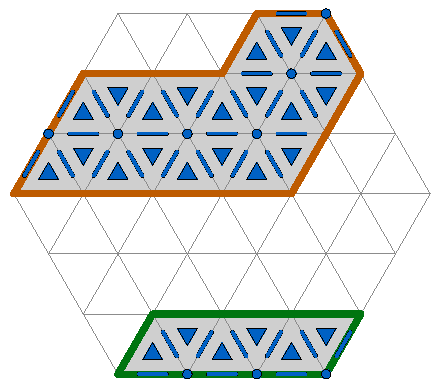
\includegraphics[width=\textwidth]{images/region_anatomy/coarse.pdf}
        \caption{A region $\R_\lzero$ with two patches (orange and green) and its open DoFs (blue markers, Def.~\ref{def:open_patch_dofs}).}
        \label{fig:region_anatomy_a}
    \end{subfigure}\hspace{10mm}
    \begin{subfigure}[t]{0.38\textwidth}
        \centering
        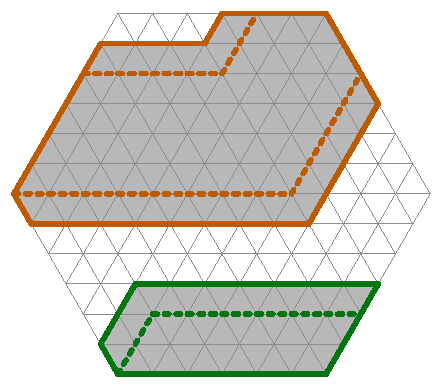
\includegraphics[width=\textwidth]{images/region_anatomy/fine.pdf}
        \caption{Refined region $\R_1 = \R_{\lzero \to 1}$ (dotted) and its extension $\extendedPatch{\R}_1$ (solid). The refinement implies $\R_\lzero = \ancestorPatch{\R_1}$.}
        \label{fig:region_anatomy_b}
    \end{subfigure}
    \caption{The geometry of regions: patches, refinement and ancestors, and extentions. While panel (a) contains the open patch DoFs, we excluded them from panel (b) to avoid visual clutter. They fill the region $\R_1$ in exactly the same way as they fill region $\R_\lzero$.}
    \label{fig:region_anatomy}
\end{figure}

Two operations on regions are used throughout and visualised in Figure~\ref{fig:region_anatomy}. We write $\FVl{\l}(\vertex{\l}{\coarseIdxone})$ for the \emph{mesh star} of $\vertex{\l}{\coarseIdxone}$, which collects all faces of the entire mesh $\T_\l$ incident to $\vertex{\l}{\coarseIdxone}$, and $\V_\l(\R_\l)$ for the vertices of the faces of the region $\R_\l$.

The first operation grows a region by one strip of faces. The \emph{extension} $\extendedPatch{\R}_\l$ of a region $\R_\l$ is
\begin{equation}
    \label{eq:patch_extension}
    \R_\l \quad \mapsto \quad \extendedPatch{\R}_\l
    \coloneq \bigcup\limits_{\vertex{\l}{\coarseIdxone} \in \V_\l(\R_\l)}
    \FVl{\l} \big(\vertex{\l}{\coarseIdxone} \big) .
\end{equation}
We refer to the faces $\extendedPatch{\R}_\l \setminus \R_\l$ added by the extension as \emph{collar}. Since the union runs over \emph{all} vertices of the region, the collar is added along the entire boundary of $\R_\l$. Figure~\ref{fig:region_anatomy_b} shows a dotted region and its extension with a solid outline. Where the region already reaches the boundary $\boundary \T_\l$ of the mesh there is nothing to add, so the collar grows only along the \emph{interface}, the part of the region boundary shared with the interior of the mesh.

The second operation passes between a region and its refinement, and it is the one that carries a constraint.

\begin{definition}[Ancestor region]
    \label{def:ancestor_patch}
    A region $\R_{\l+1} \subseteq \F_{\l+1}(\T_{\l+1})$ is \emph{quadrisection-closed} if $\R_{\l+1} = \R_{\l \to \l+1}$ for some region $\R_\l \subseteq \F_\l(\T_\l)$\guidance{, which is then unique because quadrisection is injective on face sets}. On these regions, the \emph{ancestor} operator $\ancestorPatch{\cdot}$ is defined by
    \begin{equation}
        \R_{\l+1} = \R_{\l \to \l+1} \quad \Longleftrightarrow \quad \ancestorPatch{\R_{\l+1}} = \R_{\l}.
    \end{equation}
    Writing $\ancestorPatch{\R_{\l+1}}$ therefore always carries the assumption that $\R_{\l+1}$ is quadrisection-closed.
\end{definition}

\begin{definition}[Domain sequence]
    \label{def:domseq}
    A domain sequence $\domseq[\L] \coloneq \guidance{\bigsqcup_{\l=\lzero}^{\L}} \M_\l$ is a set of regions $\M_\l$, \guidance{quadrisection-closed for every $\l > \lzero$ so that $\ancestorPatch{\M_\l}$ is defined,} that satisfy
    \begin{equation}
        \guidance{\M_\lzero = \F_\lzero(\T_\lzero)} \qquad \text{and} \qquad \ancestorPatch{\M_{\l+1}} \subseteq \M_\l.
    \end{equation}
    for $\l \in \{ \lzero, \, \dots, \, \L \}$. By convention, $\M_{\L+1} = \varnothing$. Typically each $\M_\l$ consists of several disjoint patches. The set of all domain sequences is denoted by $\alldomseqs_\L$.
\end{definition}

Regions are allowed to be empty. If $\M_{\lone} = \varnothing$ for every $\lone > \l$, the nesting condition reduces to $\varnothing \subseteq \M_{\l}$ and holds for free, so $\domseq[\L]$ is a domain sequence of $\T_\L$ whose finest faces sit on level $\l$. Thus, the single index $\L$ carries two roles at once: a maximum for $\l$ or a minimum number of smoothing steps $\L-\l$ for all basis functions (cf.~\cite{Piel.2026}). The first case simply allows basis functions to be selected across the entire hierarchy from $\T_\lzero$ to $\T_\L$. In the second case, the non-empty regions up to level $\l$ hold the selected DoFe, while $\L$ itself fixes the mesh $\T_\L$ on which every basis function is represented and thus controls the smoothing. Both can be represented using the same notation, with $\M_{\lone} = \varnothing$ for the second case.

The vertices $\V(\domseq[\L])$ of the domain sequence $\domseq[\L] = \bigsqcup_{\l = \lzero}^{\L} \M_\l$ \guidance{are} given by
\begin{equation}
    \label{eq:vertices_of_domseq}
    \V(\domseq[\L]) \; \coloneq \; \bigsqcup\limits_{\l = \lzero}^{\L} \; \V_\l(\M_\l).
\end{equation}

\smallskip

\begin{definition}[Leaf faces]
    \label{def:leaf_faces}
    Let $\domseq[\L]$ be a domain sequence of $\T_\L$. Its \emph{leaf faces} $\leafF{\l}$ are all faces of the region $\M_\l$ that are not refined beyond level $\l$, i.e.
    \begin{equation}
        \label{eq:leaf_faces}
        \leafF{\l}(\domseq[\L]) \coloneq \M_\l \setminus \ancestorPatch{\M_{\l+1}}.
    \end{equation}
\end{definition}

Definition~\ref{def:domseq} provides $\ancestorPatch{\M_{\l+1}} \subseteq \M_\l$, so Equation~\eqref{eq:leaf_faces} implies that we can split the coarse region $\M_\l$ into two named halves,
\begin{equation}
    \label{eq:leaf_ancestor_split}
    \M_\l \; = \; \leafF{\l}(\domseq[\L]) \; \sqcup \; \ancestorPatch{\M_{\l+1}},
\end{equation}
and we say that a face of $\M_\l$ is \emph{refined beyond level $\l$} when it is an element of $\ancestorPatch{\M_{\l+1}}$. This one predicate carries the rest of the construction because it decides which faces a level hands on to the next, and every geometric notion below is phrased with it.

On the other hand, leaf faces are exactly the faces that are not refined beyond their level. The leaf faces of all levels together tile the domain exactly once. We call their union
\begin{equation}
    \label{eq:leaf_mesh}
    \leafMesh(\domseq[\L]) \; \coloneq \; \bigsqcup\limits_{\l = \lzero}^{\L} \; \leafF{\l}(\domseq[\L])
\end{equation}
the \emph{leaf mesh} of $\domseq[\L]$. It is not a mesh in the strict sense because it can \guidance{have hanging nodes where faces of different levels meet}. The leaf mesh is a useful tool to represent a domain sequence in plots, see for example Figure~\ref{fig:active_dofs}, with the understanding that the coarse parents of its faces are also in the domain sequence. 

\begin{remark}[\robert{The domain sequence as a forest of quadtrees}]
    \label{rem:tree_reading}
    \robert{The two conditions of Definition~\ref{def:domseq} can be read as saying that the regions of a domain sequence form a forest of quadtrees, with one tree rooted in each face of the coarse mesh $\T_\lzero$. A face $\face{\l}{\coarseIdxone} \in \M_\l$ is a node at depth $\l$; the nesting condition supplies its parent, so no node is orphaned; and quadrisection-closedness says that an interior node carries all four of its children at once. Under this reading the two halves of the splitting~\eqref{eq:leaf_ancestor_split} are the two kinds of node: a face refined beyond its level is an interior node, and a leaf face is a node without children. This is where the name comes from, and the leaf mesh~\eqref{eq:leaf_mesh} is the set of leaves of the forest. It tiles the domain exactly once because the four children of an interior node partition it, so the leaves of each tree partition the coarse face it is rooted in.

    The forest and the leaf mesh carry the same information, and each hides what the other shows. Reading the leaf mesh recovers the regions from the finest level down, by $\M_\l = \leafF{\l}(\domseq[\L]) \cup \anc{\l}(\M_{\l+1})$, but it stores no coarse face that has been refined and shows the nesting only indirectly. The forest stores every face and makes ancestry immediate, but a tree drawn as a tree says nothing about which faces are adjacent, since adjacency is a property of the uniform mesh $\T_\l$ and not of the domain sequence. We therefore use whichever is cheaper for the statement at hand: the leaf mesh for anything about neighbourhoods, coverings and plots, and the forest for anything that walks between levels. Lemma~\ref{lemma:ancestral_closure} is the precise form of this remark, and Corollary~\ref{cor:ancestor_walk} together with Figure~\ref{fig:ancestor_walk} is where the forest does the work.}
\end{remark}

The leaf mesh also tracks the refinement frontier in the sense that \guidance{it} is a collection of the finest faces of a domain sequence that cover the faces of the domain $\T_\L$. Thus, the leaf mesh plays a large role in the definition of the refinement operators in Section~\ref{subsec:vertex_neighbourhoods}.

\guidance{Lemma~\ref{lemma:ancestral_closure} (ancestral closure of a domain sequence) and Corollary~\ref{cor:leaf_faces_terminal} (leaf faces are terminal) used to stand here, between Definition~\ref{def:leaf_faces} and the active DoFs. They are properties of domain sequences and so belong to this section by subject, but neither is used anywhere before Section~\ref{subsec:refinement_operators}: their only consumers are Lemma~\ref{lemma:ancestry_absorbed} and Corollary~\ref{cor:graded_quadrisection_leafstar}. Standing here they only delayed the reader on the way to Definition~\ref{def:active_k_form_dofs}, so both now sit at the head of Section~\ref{subsec:vertex_neighbourhoods}, directly after the face ancestor and directly before Definition~\ref{def:covering_face}, which is their first consumer. Move them back if you would rather have this section carry every property of domain sequences the paper proves.}


Now that domain sequences, regions, and their geometry are settled, we are now moving to defining active DoFs on them. \cite{companion_paper} distinguishes between two notions: the DoFs a region naturally carries, and the ones that are \emph{interior} to it in the sense that nothing outside the region touches them.

\begin{definition}[Region DoFs]
    \label{def:region_dofs}
    The DoFs $\patchDoFs{\R}{k}_\l$ of the region $\R_\l \subseteq \F_\l(\T_\l)$ are given by $\patchDoFs{\R}{k}_\l \coloneq \K^k_\l(\R_\l)$, i.e. all $k$-simplices that contained in at least of face of the region.
\end{definition}

\begin{definition}[Open region DoFs]
    \label{def:open_patch_dofs}
    Let $\R_\l \subseteq \T_\l$ be a region. A region DoF $\patchDoFs{\R}{k}_\l$ is \emph{open} when every face containing it belongs to $\R_\l$. Thus, the open region DoFs $\openPatchDoFs{\R}{k}_\l$ of $\R_\l$ are given by
    \begin{equation}
        \label{eq:open_dofs_membership}
        \openPatchDoFs{\R}{k}_\l \coloneq \big\{ \simplex{k}{\l}{\coarseIdxone} \in \patchDoFs{\R}{k}_\l
        \; : \; \F\K^k_\l\big(\simplex{k}{\l}{\coarseIdxone}\big) \subseteq \R_\l \big\}.
    \end{equation}
\end{definition}

Equation~\eqref{eq:open_dofs_membership} is the form of the definition we work with because it is
a purely local test on the faces containing a simplex, with no reference to interfaces or to
neighbouring regions; it is shown in~\cite{companion_paper} to agree with the region DoFs less
those carried by the interface of $\R_\l$. The test is the right one at the mesh boundary as well:
a simplex on $\boundary\T_\l$ is open in $\R_\l$ as soon as the faces on its single side belong to
$\R_\l$, so a region reaching the mesh boundary is not stripped there.
Figure~\ref{fig:region_anatomy_a} carries out the test on a region:
the marked simplices are the open ones, and the vertices where two patches meet or where the
region ends are the ones it rejects.

\begin{definition}[Active $k$-form degrees of freedom]
    \label{def:active_k_form_dofs}
    Let $\domseq[\L] = \guidance{\bigsqcup_{\l = \lzero}^{\L}} \M_\l$ be a domain sequence of $\T_\L$. The
    active $k$-form degrees of freedom $\activeDoFSet{k}{}(\domseq[\L])$ are defined level by
    level as
    \begin{equation}
        \label{eq:active_k_form_dofs}
        \activeDoFSet{k}{} (\domseq[\L]) \coloneq \bigsqcup\limits_{\l = \lzero}^{\L} \; \activeDoFSet{k}{\l}, \qquad \text{where} \qquad \activeDoFSet{k}{\l} = \big( \openPatchDoFs{\extendedPatch{\M}}{k}_\l \setminus \openPatchDoFs{\ancestorPatch{\M_{\l+1}}}{k}_\l \big),
    \end{equation}
    where $\openPatchDoFs{\extendedPatch{\M}}{k}_\l$ are the open DoFs of the extended region $\M_\l$ that are added on level $\l$, and $\openPatchDoFs{\ancestorPatch{\M_{\l+1}}}{k}_\l$ are the open patch DoFs of the ancestor patch of $\M_{\l+1}$ that are removed on level $\l$ because $\M_{\l+1}$ will add finer DoFs there in the next step. Further, we define the active $k$-form degrees of freedom $\activeDoFSetZero{k}{}$ without boundary degrees of freedom by
    \begin{equation}
        \activeDoFSetZero{k}{} (\domseq[\L]) \coloneq \bigsqcup\limits_{\l = \lzero}^{\L} \; \activeDoFSetZero{k}{\l}, \qquad \text{where} \qquad \activeDoFSetZero{k}{\l} = \activeDoFSet{k}{\l} \setminus \K^k_\l(\partial \T_\l).
    \end{equation}
\end{definition}

% ============================================================
%  Grid of active DoFs: columns are levels, rows are form degrees, with the
%  domain sequence beside the grid rather than stacked above it. Everything left
%  of the grid is placed by explicit coordinate so the domain sequence sits on
%  the brace's midline, and stays there if the panel size changes.
% ============================================================
\begin{figure}[tb]
\begin{center}
\begin{tikzpicture}[
    every node/.style={inner sep=0pt, outer sep=0pt}
]

% Panels are 0.21\textwidth = 3.36cm wide and, at the generator's 90.71:79.24
% aspect, 2.94cm tall -- so columns must clear 3.36cm and rows 2.94cm.
\def\panelw{0.21\textwidth}
\def\cA{0cm}     \def\cB{3.65cm}  \def\cC{7.3cm}
\def\rA{0cm}     \def\rB{-3.2cm}  \def\rC{-6.4cm}
% x positions left of the grid, and the vertical centre of the grid
\def\xK{-2.15cm} \def\xBrace{-2.55cm} \def\xBlab{-3.2cm} \def\xPart{-5.05cm}
\def\yMid{-3.2cm}

% ---- grid: columns are levels, rows are form degrees -------------------
\node (P00) at (\cA, \rA) {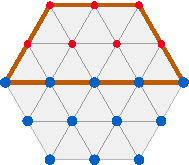
\includegraphics[width=\panelw]{images/dofmeshes/two_level_interface/dofs_k_0_lvl_l0.pdf}};
\node (P01) at (\cB, \rA) {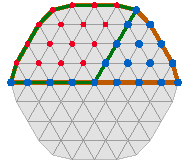
\includegraphics[width=\panelw]{images/dofmeshes/two_level_interface/dofs_k_0_lvl_l1.pdf}};
\node (P02) at (\cC, \rA) {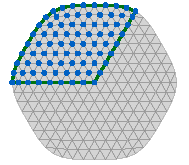
\includegraphics[width=\panelw]{images/dofmeshes/two_level_interface/dofs_k_0_lvl_l2.pdf}};

\node (P10) at (\cA, \rB) {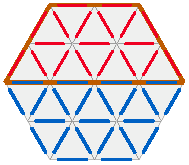
\includegraphics[width=\panelw]{images/dofmeshes/two_level_interface/dofs_k_1_lvl_l0.pdf}};
\node (P11) at (\cB, \rB) {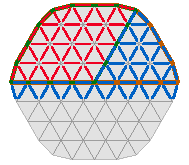
\includegraphics[width=\panelw]{images/dofmeshes/two_level_interface/dofs_k_1_lvl_l1.pdf}};
\node (P12) at (\cC, \rB) {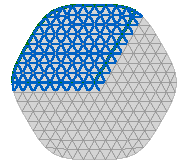
\includegraphics[width=\panelw]{images/dofmeshes/two_level_interface/dofs_k_1_lvl_l2.pdf}};

\node (P20) at (\cA, \rC) {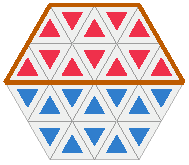
\includegraphics[width=\panelw]{images/dofmeshes/two_level_interface/dofs_k_2_lvl_l0.pdf}};
\node (P21) at (\cB, \rC) {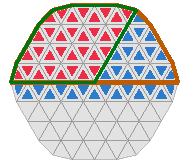
\includegraphics[width=\panelw]{images/dofmeshes/two_level_interface/dofs_k_2_lvl_l1.pdf}};
\node (P22) at (\cC, \rC) {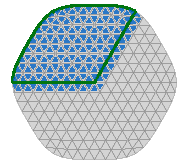
\includegraphics[width=\panelw]{images/dofmeshes/two_level_interface/dofs_k_2_lvl_l2.pdf}};

% ---- column labels (levels), row labels (form degrees, rotated) --------
\node[above=6pt of P00, font=\bfseries, inner sep=2pt] {$\l = 0$};
\node[above=6pt of P01, font=\bfseries, inner sep=2pt] {$\l = 1$};
\node[above=6pt of P02, font=\bfseries, inner sep=2pt] {$\l = 2$};

\node[font=\bfseries, rotate=90] at (\xK, \rA) {$k = 0$};
\node[font=\bfseries, rotate=90] at (\xK, \rB) {$k = 1$};
\node[font=\bfseries, rotate=90] at (\xK, \rC) {$k = 2$};

% ---- brace, opening towards the domain sequence on the left ------------
\draw[
    decoration={calligraphic brace, amplitude=6pt, raise=4pt},
    decorate, line width=1.2pt
]
    (\xBrace, {\rC-1.47cm}) -- (\xBrace, {\rA+1.47cm});

\node[font=\bfseries, rotate=90] at (\xBlab, \yMid) {active DoFs};

% ---- the domain sequence, centred on the brace -------------------------
\node (partfig) at (\xPart, \yMid)
    {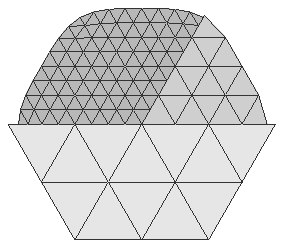
\includegraphics[width=0.19\textwidth]{images/dofmeshes/two_level_interface/subdiv_partition.pdf}};

\node[below=4pt of partfig, align=center] {domain sequence};

\end{tikzpicture}
\end{center}
\caption{Active $k$-form DoFs for the domain sequence on the left, represented through its leaf mesh. The grey shading indicates the level of the leaf faces. The orange and green outlines show the regions $\M_1$ and $\M_2$, respectively, and their ancestors on the previous level. Columns correspond to the level $\l \in \{0, 1, 2\}$, rows to the form degree $k$. Each panel shows the entire uniform mesh $\T_\l$ of its level together with the DoFs of that level. Definition~\ref{def:active_k_form_dofs} selects the DoFs level by level. The blue DoFs indicate the active DoFs at the end of the selection, while the red ones were removed because the region carrying them is refined beyond its level.}
\label{fig:active_dofs}
\end{figure}

The following example explains the selection of the active DoFs for a given domain sequence in more detail.

\begin{example}
    \label{ex:selection}
    Consider the domain sequence shown on the left of Figure~\ref{fig:active_dofs}, in which $\M_0 = \T_0$ is the whole coarse mesh, $\M_1$ is its upper half, and $\M_2$ consists of the two left-most spoke regions of that half. The figure represents the domain sequence by plotting only its leaf faces, see Definition~\ref{def:leaf_faces}. That means that we read the level $2$ region $\M_2$ on the top left as also carrying a level $0$ and level $1$ component because $\ancestorPatch{\M_{\l+1}} \subseteq \M_{\l}$.

    Read the selection one level at a time, in the order of the union in Definition~\ref{def:active_k_form_dofs}. At the coarsest level $\l = 0$ the region is the whole mesh, so $\extendedPatch{\M}_0 = \T_0$. Thus, all patch DoFs of $\extendedPatch{\M}_0$ are interior and all DoFs of $\K^k_0$ are added (blue). Since $\ancestorPatch{\M_1}$ covers the top half of the domain, all DoFs interior to it are removed (red).

    At $\l = 1$, the inserted DoFs are those interior to $\extendedPatch{\M}_1$, and the removed DoFs are those interior to $\ancestorPatch{\M_2}$, the level-$1$ faces that $\M_2$ refines. Column $\l = 1$ shows exactly this. This leads to the appearance of DoFs on level $1$ along the interface between $\M_1$ and $\M_0$. These \emph{interface DoFs} survive the removal because they are not interior to $\ancestorPatch{\M_2}$. The interface DoFs are vital to ensure the differential complex, and omitting them would violate the structure-preservation, see~\cite{companion_paper}.

    At the finest level $\l = 2$ nothing is refined beyond the level, so $\ancestorPatch{\M_3} =
    \varnothing$ and nothing is removed. The active DoFs are exactly those interior to the
    extended patch $\extendedPatch{\M}_2$.
\end{example}

We now have an algorithm to select active DoFs through a domain sequence and can specify Definition~\ref{def:generic_adaptive_function_spaces} to use those DoFs.

\begin{definition}[Adaptive subdivision $k$-form spaces induced by a domain sequence]
    \label{def:adaptive_function_spaces}
    Let $\domseq[\L]$ be a domain sequence of $\T_\L$. The adaptive subdivision $k$-form spaces $\hierSDFspace{k}{\domseq}{\L}$ and $\hierSDFspaceZero{k}{\domseq}{\L}$ (with vanishing trace) induced by it are given by
    \begin{equation}
        \hierSDFspace{k}{\domseq}{\L} \coloneqq \mathrm{span}\big( \constrVec{\SDFbases}{k}{\activeDoFSet{k}{}(\domseq[\L])}{\L} \big) \qquad \text{and} \qquad \hierSDFspaceZero{k}{\domseq}{\L} \coloneqq \mathrm{span}\big( \constrVec{\mathring{\SDFbases}}{k}{\activeDoFSet{k}{}(\domseq[\L])}{\L} \big),
    \end{equation}
    where the sets $\constrVec{\SDFbases}{k}{\activeDoFSet{k}{}(\domseq[\L])}{\L}$ and $\constrVec{\mathring{\SDFbases}}{k}{\activeDoFSet{k}{}(\domseq[\L])}{\L} \coloneq \constrVec{\SDFbases}{k}{\activeDoFSetZero{k}{}(\domseq[\L])}{\L}$ of active basis functions are constructed as in Definition~\ref{def:generic_adaptive_function_spaces}.
\end{definition}

\begin{theorem}[Differential complex, from~\cite{companion_paper}]
    \label{theorem:differential_complex}
    Let $\domseq[\L]$ be a domain sequence of the mesh $\T_\L$. The adaptive subdivision $k$-form spaces $\hierSDFspace{k}{\domseq}{\L}$ constitute the differential complex
    \begin{equation}
    \begin{tikzcd}
        \mathfrak{R}_{\domseq}: \qquad 0 \arrow[r] & \hierSDFspace{0}{\domseq}{\L} \arrow[r, "\extd"] & \hierSDFspace{1}{\domseq}{\L} \arrow[r, "\extd"] & \hierSDFspace{2}{\domseq}{\L} \arrow[r] & 0.
    \end{tikzcd}
    \end{equation}
    The spaces $\hierSDFspaceZero{k}{\domseq}{\L}$ with vanishing traces form the differential complex
    \begin{equation}
    \begin{tikzcd}
        \mathring{\mathfrak{R}}_{\domseq}: \qquad 0 \arrow[r] & \hierSDFspaceZero{0}{\domseq}{\L} \arrow[r, "\extd"] & \hierSDFspaceZero{1}{\domseq}{\L} \arrow[r, "\extd"] & \hierSDFspaceZero{2}{\domseq}{\L} \arrow[r] & 0.
    \end{tikzcd}
    \end{equation}
\end{theorem}

The other essential properties of the adaptive $k$-form subdivision spaces, namely linear independence and correct cohomology of the discrete complex, are tied to the geometry of the regions that constitute the domain sequence, see~\cite{companion_paper}. This will be the subject of the following Section~\ref{subsec:subdiv_partition}.

\FloatBarrier

\subsection{Admissible domain sequences and properties of the adaptive spaces}
\label{subsec:subdiv_partition}

% --- Figure knobs: leaf star, quadrisection, and interior-vertex examples (single row, no dividers) ---
\newcommand{\cvScale}{0.22}
% #1 (optional) panel width as a fraction of \textwidth, default \cvScale --
% override per panel when its image has a different aspect ratio (e.g. a
% colorbar widens the PDF at the same height) and would otherwise come out
% shorter/taller than the rest once every panel is fit to the same width.
\newcommand{\cvsubfig}[4][\cvScale]{% #1 width fraction  #2 image path  #3 caption  #4 label
    \begin{subfigure}[t]{#1\textwidth}
        \centering
        \includegraphics[width=\textwidth]{#2}
        \caption{#3}
        \label{#4}
    \end{subfigure}%
}
\begin{figure}[tb]
    \centering
    \cvsubfig
        {images/visualisations/v6_boundary_threenotches_lvl1_lvl0_partition.pdf}
        {$\M_\lzero$ splits into leaf faces $\leafF{\lzero}$ and the ancestor patch $\ancestorPatch{\M_1}$ (purple), cf. Definition~\ref{def:leaf_faces}.}
        {fig:adm_partition}
    \hfill
    \cvsubfig
        {images/visualisations/v6_boundary_threenotches_lvl1_lvl0_refinement_fan.pdf}
        {The refinement fan (purple) as a subset of the incident faces (outlined) of a vertex on level $0$.}
        {fig:adm_fan}
    \hfill
    \cvsubfig[0.2613]
        {images/visualisations/v6_nested_center_lvl3_exterior_levels.pdf}
        {Domain sequence with its vertices coloured by the level at which they become refinement-exterior.}
        {fig:adm_exterior}
    \hfill
    \cvsubfig
        {images/visualisations/v6_boundary_threenotches_lvl1_lvl0_admissible_faces.pdf}
        {Unconfined (green) and confined (orange) leaf faces on level $\lzero$, with refinement-exterior vertices (hollow).}
        {fig:adm_faces}
    \caption{The definition chain of this section read off a single domain sequence. Purple faces indicate the ancestor $\ancestorPatch{\M_{\l+1}}$ throughout, and thus marks the faces that are refined beyond the level we compute the predicates on. Panel~\subref{fig:adm_partition} shows the input the predicates use, namely the split~\eqref{eq:leaf_ancestor_split} of $\M_\l$ into the leaf faces $\leafF{\l}(\domseq)$ and the ancestor patch $\ancestorPatch{\M_{\l+1}}$. Panel~\subref{fig:adm_fan} uses that splitting to find the refinement fan $\refFan{\lzero}$ of a vertex, see Definition~\ref{def:refinement_fan}. Panel~\subref{fig:adm_exterior} marks every vertex of a different domain sequence with nested refinement by the level at which its refinement fan first becomes empty, i.e. from which it is refinement-exterior according to Definition~\ref{def:refinement_exterior_vertex}. Panel~\subref{fig:adm_faces} visualises the split of the leaf faces on level $0$ into unconfined (green) and confined (orange) by Definition~\ref{def:confined_face}. The criterion is whether a leaf face contains at least one refinement-exterior vertex, drawn hollow.}
    \label{fig:admissibility_chain}
\end{figure}

Section~\ref{subsec:selecting_active_dofs} selects the active DoFs of level $\l$ by the subtraction in Equation~\eqref{eq:active_k_form_dofs}: the open DoFs of the extended region $\extendedPatch{\M}_\l$, minus the open DoFs of the ancestor patch $\ancestorPatch{\M_{\l+1}}$, which the next level re-supplies at half the mesh size. This exchange of DoFs being clean in the right sense is what guarantees linear independence and the correct cohomology for the adaptive subdivision $k$-form spaces, see~\cite{companion_paper}. It is clean as long as the refined and extended region $\guidance{\extendedPatch{\M}_{\l+1}}$ \guidance{does not merge patches that are disconnected in} the ancestor region $\ancestorPatch{\M_{\l+1}}$. Looking at Figure~\ref{fig:region_anatomy}, we can see that this merging could happen when patches of $\ancestorPatch{\M_{\l+1}}$ would meet in one vertex or have only one strip of coarse faces between, since the extension would bridge that gap. The admissibility conditions presented in this section can be understood as enforcing a minimum distance between two patches to avoid these problematic geometries.

The geometric predicates of this section are local tests for the ways that distance can collapse. All of are read off a single object, the \emph{refinement fan} of a vertex, which collects the faces of the mesh at that vertex that the sequence refines beyond the current level.

\begin{definition}[Refinement fan]
    \label{def:refinement_fan}
    Let $\domseq[\L]$ be a domain sequence with regions $\M_\l$. The \emph{refinement fan} $\refFan{\l} \big( \vertex{\l}{\coarseIdxone} \big)$ of a vertex $\vertex{\l}{\coarseIdxone} \in \V_\l(\T_\l)$ contains all incident faces of $\vertex{\l}{\coarseIdxone}$ that are refined beyond level $\l$ in the domain sequence, i.e.
    \begin{equation}
        \refFan{\l} \big( \vertex{\l}{\coarseIdxone} \big) \coloneq \FVl{\l} \big( \vertex{\l}{\coarseIdxone} \big) \cap \ancestorPatch{\M_{\l+1}}.
    \end{equation}
\end{definition}

An empty refinement fan implies that vertex at level $\l$ is outside of the region $\ancestorPatch{\M_{\l+1}}$ of $\domseq[\L]$, and thus exterior to any refinement beyond $\l$. The following definition formalises that idea.

\begin{definition}[Refinement-exterior vertex]
    \label{def:refinement_exterior_vertex}
    Let $\domseq[\L]$ be a domain sequence. A vertex $\vertex{\l}{\coarseIdxone} \in \V_\l(\T_\l)$ is \emph{refinement-exterior} at level $\l$ if its refinement fan in $\domseq[\L]$ is empty on that level, i.e. $\refFan{\l} \big( \vertex{\l}{\coarseIdxone} \big) = \varnothing$.
\end{definition}

Note that a refinement-exterior vertex of $\domseq[\L]$ at a given level $\l$ need not be in the interior of $\T_\l$ but can also lie on its boundary $\partial \T_\l$. For example, Figures~\ref{fig:adm_exterior} and~\ref{fig:adm_faces} display domain sequences with refinement-exterior vertices at the domain boundary.

The refinement fan can only empty out. \guidance{If none of a vertex' incident faces lies in $\ancestorPatch{\M_{\l+1}}$, then no face of $\M_{\l+1}$ contains it either, since each of those sits inside a coarse face that does not. The collar of the extension adds one strip of level-$(\l+1)$ faces, which is half a coarse face wide and therefore too narrow to bridge that gap, so the vertex stays outside $\extendedPatch{\M}_{\l+1}$ as well.} Thus, a vertex that is refinement-exterior at one level stays refinement-exterior at all finer ones. Every vertex therefore has a level at which it first becomes refinement-exterior, which is what Figure~\ref{fig:adm_exterior} colours it by. In this figure, the outermost layer is refinement-exterior already at level $\lzero$, because none of its incident faces is refined beyond that level, so its refinement fan is empty there according to Definition~\ref{def:refinement_fan}. The next layer becomes refinement-exterior only at level $1$, since at level $0$ it still has incident faces that are refined beyond that level. This logic applies to all layers in the figure until we reach the finest level $3$, at which the remaining vertices become refinement-exterior.

\smallskip

% OLD (pre-rename), delete once cherry-picked:
% The first geometric predicate concerns a leaf face enclosed by refinement. If none of its vertices is refinement-exterior, the finer level extension reaches the coarse face from every corner at once, which can lead to linear dependence or merging patches. The predicate names the harmless complement.
\guidance{The first geometric predicate concerns a leaf face that the refinement has closed in on. If none of its vertices is refinement-exterior, all of its corners lie in $\ancestorPatch{\M_{\l+1}}$ and the finer level extension reaches the coarse face from every corner at once, which can lead to linear dependence or merging patches. The predicate calls such a face confined.}

\begin{definition}[Confined face]
    \label{def:confined_face}
    \guidance{A leaf face $\face{\l}{\coarseIdxone} \in \leafF{\l}(\domseq[\L])$} is \emph{unconfined} if at least one of its vertices is refinement-exterior at level $\l$. Otherwise, it is \emph{confined}.
\end{definition}

The second problematic configuration is a vertex at which the refined part of its mesh star falls into two or more distinct patches meeting only at the vertex itself. The coarse faces that separate them are squeezed to a point there, so the extended refined patches are guaranteed to merge. \guidance{Counting these patches is what the next two definitions do.}

\begin{definition}[Refinement arcs of a vertex]
    \label{def:refinement_arcs}
    Let $\vertex{\l}{\coarseIdxone} \in \V(\domseq[\L])$. The \emph{refinement arcs of $\vertex{\l}{\coarseIdxone}$} are the maximal runs of consecutive faces in its cyclic (or, at a boundary vertex, linear) refinement fan $\refFan{\l}(\vertex{\l}{\coarseIdxone})$. \guidance{Two faces of the same arc are connected by a chain of faces of the fan, consecutive ones sharing a level-$\l$ edge at $\vertex{\l}{\coarseIdxone}$, while faces of distinct arcs are not. The maximal runs of $\FVl{\l}(\vertex{\l}{\coarseIdxone})$ that are \emph{not} in $\refFan{\l}(\vertex{\l}{\coarseIdxone})$ are the \emph{gaps} of $\vertex{\l}{\coarseIdxone}$, cyclic at an interior vertex and linear at a boundary vertex.}
\end{definition}

\begin{definition}[Pinch vertex]
    \label{def:pinch_vertex}
    A vertex $\vertex{\l}{\coarseIdxone} \in \V(\domseq[\L])$ is a \emph{pinch vertex} if it has two or more refinement arcs.
\end{definition}

At the domain boundary the same defect takes a second form that the number of pieces alone does not see. A single fine boundary vertex can be sealed off by coarse faces on both sides and touch the boundary only through the vertex. In that case, the open DoFs strip the single boundary vertex, while the open DoFs of the refined and extended version carry a boundary component.

\begin{definition}[Boundary pinch vertex]
    \label{def:boundary_pinch}
    Let $\vertex{\l}{\coarseIdxone} \in \V(\domseq[\L]) \cap \partial\T_\l$ lie on the boundary of $\T_\l$. \guidance{Exactly two faces of its mesh star $\FVl{\l}(\vertex{\l}{\coarseIdxone})$ carry a domain boundary edge incident to $\vertex{\l}{\coarseIdxone}$, namely the two ends of its linear fan. We call a refinement arc \emph{anchored} if it contains one of them.} The vertex $\vertex{\l}{\coarseIdxone}$ is a \emph{boundary pinch} if it has at least one refinement arc that is not anchored.
\end{definition}

% --- Figure knobs: admissibility predicates on concrete domain sequences (single row, no dividers) ---
\newcommand{\admScale}{0.23}
\newcommand{\admsubfig}[3]{% #1 image path  #2 caption  #3 label
    \begin{subfigure}[t]{\admScale\textwidth}
        \centering
        \includegraphics[width=\textwidth]{#1}
        \caption{#2}
        \label{#3}
    \end{subfigure}%
}
% -------------------------------------------------------------------------
\begin{figure}[tb]
    \centering
    \admsubfig
        {images/visualisations/v8_quarters_lvl1_pinch_marked.pdf}
        {Interior pinch with two refinement arcs}{fig:pinch_interior}
    \hfill
    \admsubfig
        {images/visualisations/v8_graded_top_bottom_sides_pinch_marked.pdf}
        {Non-pinch with a single refinement arc}{fig:pinch_single_arc}
    \hfill
    \admsubfig
        {images/visualisations/v6_boundary_topbottom_lvl1_pinch_marked.pdf}
        {Pinches at the domain boundary}{fig:pinch_boundary_two_arcs}
    \hfill
    \admsubfig
        {images/visualisations/v6_boundary_triangle_lvl1_pinch_marked.pdf}
        {Boundary pinches with unanchored arcs}{fig:pinch_boundary_unanchored}
    \caption{Four domain sequences (represented by their leaf mesh) with the potential pinch vertex marked in yellow and the faces of its refinement arcs shaded in purple, cf. Definitions~\ref{def:pinch_vertex} and~\ref{def:boundary_pinch}. Panels~\subref{fig:pinch_boundary_two_arcs} and~\subref{fig:pinch_boundary_unanchored} visualise one additional subtlety: boundary vertices can create pinches in two distinct ways, either by two refinement arcs as in~\subref{fig:pinch_boundary_two_arcs} or by one unanchored refinement arc as in~\subref{fig:pinch_boundary_unanchored}. The former case is considered an interior pinch that happens at the boundary, while the letter is considered a bondary pinch.}
    \label{fig:pinches}
\end{figure}

\smallskip

The predicates of face confinement and vertex pinches allow us to define \emph{admissible domain sequences} as a subset of domain sequences.

\begin{definition}[Admissible domain sequence]
    \label{def:subdiv_partition}
    A domain sequence $\domseq[\L](\T_\L)$ is an \emph{admissible domain sequence} iff
    \begin{itemize}
        \item[(i)] no leaf face of $\domseq[\L]$ is confined,
        \item[(ii)] no vertex of $\domseq[\L]$ is a pinch vertex,
        \item[(iii)] no domain boundary vertex of $\domseq[\L]$ is a boundary pinch vertex.
    \end{itemize}
    We denote the set of admissible domain sequences by $\allpartitions(\T_\L)$.
\end{definition}

Condition (ii) is deliberately not restricted to interior vertices to cover cases like the one in Figure~\ref{fig:pinch_boundary_two_arcs}. The three conditions are the three collapses ruled out one by one, \guidance{so together they keep distinct patches of $\ancestorPatch{\M_{\l+1}}$ far enough apart for the exchange of Section~\ref{subsec:selecting_active_dofs}, stated entirely in terms of one vertex or one face at a time, and~\cite{companion_paper} proves that they suffice.} 

The following two theorems are from ~\cite{companion_paper} and show that both linear independence and the correct cohomology of the adaptive subdivision $k$-form spaces follow from the admissibility of the domain sequence they are defined on.

\begin{theorem}[Linear independence, from~\cite{companion_paper}]
    \label{theorem:linear_independence}
    Let $\domseq \in \allpartitions$ be a admissible domain sequence of the mesh $\T_\L$. The active basis functions selected by Def.~\ref{def:active_k_form_dofs} of the adaptive spaces $\hierSDFspace{k}{\domseq}{\L}$ are linearly independent.
\end{theorem}

The minimum gap between two patches enforced by the admissibility of the domain sequence also guarantees that the regions preserve their respective cohomology classes under refinement and extension, see~\cite{companion_paper} for a detailed derivation.

\begin{theorem}[Discrete de Rham complexes, from~\cite{companion_paper}]
    \label{theorem:exactness}
    Let $\domseq \in \allpartitions$ be a admissible domain sequence. Then, the cohomology groups of the complexes $\mathfrak{R}_{\domseq}$ and $\mathring{\mathfrak{R}}_{\domseq}$ of adaptive $k$-form subdivision spaces from Theorem~\ref{theorem:differential_complex} are isomorphic to the ones of absolute and relative de Rham complexes, respectively.
\end{theorem}


\FloatBarrier

\subsection{Vertex neighbourhoods for the refinement operators}
\label{subsec:vertex_neighbourhoods}

The previous section constrained the domain sequence. This section and the next one build the machinery that carries our adaptive loop from one admissible domain sequence to a finer one, so the definitions from here on are answerable to the algorithm rather than to the theorems, meaning that they are chosen so that the operators of Section~\ref{subsec:refinement_operators} can be stated and implemented, and a different refinement strategy would replace them while leaving Section~\ref{subsec:subdiv_partition} untouched.

This section defines three neighbourhoods of a vertex, and they differ in what they are allowed to read. The \emph{mesh star} $\FVl{\l}(\vertex{\l}{\coarseIdxone})$ of Section~\ref{subsec:selecting_active_dofs} collects the faces of $\T_\l$ incident to $\vertex{\l}{\coarseIdxone}$ and is a property of the uniform mesh alone, but it is only defined on the levels at which the vertex is a mesh vertex. The \emph{star ancestry} below removes that restriction while staying a property of the mesh hierarchy alone. The \emph{leaf star} defined afterwards is the only one of the three that reads the domain sequence.

\begin{definition}[Face ancestor]
    \label{def:face_ancestor}
    Let $\face{\lone}{\coarseIdxone} \in \F_\lone(\T_\lone)$ be a face on level $\lone$ and choose a coarser level $\l$ such that $\lzero \leq \l \leq \lone$. The \emph{face ancestor} operator $\anc{\l}$ sends $\face{\lone}{\coarseIdxone}$ to its ancestor $\face{\l}{\fineIdxone}$ on level $\l$ by the identity
    \begin{equation}
        \label{eq:face_ancestor}
        \anc{\l} \big( \face{\lone}{\coarseIdxone} \big) = \face{\l}{\fineIdxone} \quad \Longleftrightarrow \quad \face{\lone}{\coarseIdxone} \in \Aop{}{\l}{\lone} \big( \face{\l}{\coarseIdxone} \big).
    \end{equation}
    The face ancestor operator extends to sets $\simplexsubset{2}{\lone} \in \F_{\lone}(\T_\lone)$ of faces on level $\lone$ by
    \begin{equation}
        \anc{\l}(\simplexsubset{2}{\lone}) = \bigcup_{\face{\lone}{\coarseIdxone} \in \simplexsubset{2}{\lone}} \; \anc{\l} \big(\face{\lone}{\coarseIdxone} \big).
    \end{equation}
\end{definition}


Both the face ancestor and the patch ancestor only operator on mesh hierarchy, not on a domain sequence. The difference between them is that face ancestor operator only needs ``$\in$'' instead of the ``$=$'' in Definition~\ref{def:ancestor_patch} of the ancestor patch. This is why the patch ancestor carries the assumption of quadrisection-closedness, while the face ancestor does not require that.

Face Ancestry composes, i.e. $\anc{\l} \circ \anc{\lone} (\face{\ltwo}{\coarseIdxone}) = \anc{\l} (\face{\ltwo}{\coarseIdxone})$ for $\l \leq \lone \leq \ltwo$, and $\anc{\lone}(\face{\lone}{\coarseIdxone}) = \face{\lone}{\coarseIdxone}$ is the identity. Refining and then coarsening returns the argument, i.e. $\anc{\l}(\Aop{}{\l}{\lone} \, \simplexsubset{2}{\l}) = \simplexsubset{2}{\l}$, because quadrisection is injective on face sets. The other composition does not, since $\anc{\l}$ keeps a coarse face as soon as only one of its children is present, and that is precisely where the face ancestor differs from the ancestor region $\ancestorPatch{\cdot}$ of Definition~\ref{def:ancestor_patch}. The two agree wherever $\ancestorPatch{\cdot}$ is defined,
\begin{equation}
    \label{eq:ancestor_patch_is_anc}
    \ancestorPatch{\simplexsubset{2}{\l+1}} \; = \; \anc{\l} ( \simplexsubset{2}{\l+1} ) \qquad \text{for quadrisection-closed} \qquad \simplexsubset{2}{\l+1}.
\end{equation}
We keep both, because $\ancestorPatch{\cdot}$ carries that hypothesis in its notation, which is what makes the nesting condition of Definition~\ref{def:domseq} readable, while $\anc{\l}$ is what the neighbourhoods below need since a mesh star is not quadrisection-closed.

\begin{lemma}[Ancestral closure of a domain sequence]
    \label{lemma:ancestral_closure}
    Let $\domseq[\L] \in \alldomseqs_\L$ with regions $\M_\lone$ and let $\lzero \leq \l < \lone \leq \L$. Every face of $\M_\lone$ has its level-$\l$ ancestor refined beyond level $\l$,
    \begin{equation}
        \label{eq:ancestral_closure}
        \anc{\l} \big( \simplexsubset{2}{\lone} \big) \; \subseteq \; \ancestorPatch{\M_{\l+1}} \; \subseteq \; \M_\l \qquad \text{for every} \qquad \simplexsubset{2}{\lone} \subseteq \M_\lone.
    \end{equation}
\end{lemma}
\begin{proof}
    The face ancestor operator acts facewise by Definition~\ref{def:face_ancestor}, so it suffices to walk a single face $\face{\lone}{\fineIdxone} \in \simplexsubset{2}{\lone} \subseteq \M_\lone$ down one level at a time. Let $\lzero \leq \l < \lone$ and suppose $\anc{\l+1}(\face{\lone}{\fineIdxone}) \in \M_{\l+1}$. Since $\l \geq \lzero$, Definition~\ref{def:domseq} makes $\M_{\l+1}$ quadrisection-closed, that is $\M_{\l+1} = \Aop{}{\l}{\l+1}(\ancestorPatch{\M_{\l+1}})$, so $\anc{\l+1}(\face{\lone}{\fineIdxone})$ is a child of a face of $\ancestorPatch{\M_{\l+1}}$, which can only be its parent $\anc{\l}(\face{\lone}{\fineIdxone})$. The nesting condition of the same definition carries that parent on into $\M_\l$. This is the assertion on level $\l$ and the supposition one level further down, and it starts at $\l = \lone \! - \! 1$ because $\face{\lone}{\fineIdxone} \in \M_\lone$.
\end{proof}

Read in reverse, Lemma~\ref{lemma:ancestral_closure} says that a face which fails to be refined beyond its level cuts off the hierarchy below it. This is the sense in which leaf faces are the frontier and not merely the currently finest thing present.

\begin{corollary}[Leaf faces are terminal]
    \label{cor:leaf_faces_terminal}
    Let $\domseq[\L] \in \alldomseqs_\L$ and let $\face{\l}{\fineIdxone} \in \leafF{\l}(\domseq[\L])$ be a leaf face. Then no descendant of $\face{\l}{\fineIdxone}$ lies in any region of $\domseq[\L]$,
    \begin{equation}
        \label{eq:leaf_faces_terminal}
        \Aop{}{\l}{\lone} \big( \face{\l}{\fineIdxone} \big) \, \cap \, \M_\lone \; = \; \varnothing \qquad \text{for all} \qquad \l < \lone \leq \L.
    \end{equation}
\end{corollary}
\begin{proof}
    Suppose some descendant $\face{\lone}{\fineIdxtwo} \in \Aop{}{\l}{\lone}(\face{\l}{\fineIdxone})$ lay in $\M_\lone$. Its level-$\l$ ancestor is $\face{\l}{\fineIdxone}$, so Lemma~\ref{lemma:ancestral_closure} would give $\face{\l}{\fineIdxone} \in \ancestorPatch{\M_{\l+1}}$, contradicting $\face{\l}{\fineIdxone} \in \leafF{\l}(\domseq[\L]) = \M_\l \setminus \ancestorPatch{\M_{\l+1}}$ of Definition~\ref{def:leaf_faces}.
\end{proof}


\begin{definition}[Covering face]
    \label{def:covering_face}
    Let $\domseq[\L] \in \alldomseqs$ and let $\face{\lone}{\fineIdxone} \in \F_{\lone}(\T_\lone)$ be a face on level $\lone$. The \emph{covering face} of $\face{\lone}{\fineIdxone}$ is the one face ancestor of $\face{\lone}{\fineIdxone}$ that is a leaf face,
    \begin{equation}
        \label{eq:covering_face}
        \coveringFace \big( \face{\lone}{\fineIdxone} \big) \; \coloneq \; \anc{\l} \big( \face{\lone}{\fineIdxone} \big) \qquad \text{for the level } \l \text{ with } \; \anc{\l} \big( \face{\lone}{\fineIdxone} \big) \, \in \, \leafMesh(\domseq[\L]) .
    \end{equation}
    At most one level meets that condition, and we set $\coveringFace(\face{\lone}{\fineIdxone}) \coloneq \varnothing$ when none does. The next two results show both, and identify the faces for which no level qualifies.
\end{definition}

% ============================================================
% fig:ancestor_walk -- hand-authored schematic, NOT generated. There is no
% domain sequence to read here: the point is combinatorial, so the figure is
% the face quadtree and not a mesh. Drawn in TikZ for that reason, and because
% the arrow labels are then the real macros ($\anc{\l}$, $\Aop{}{\l}{\l+1}$)
% set in the document font.
%
% Layout knobs. Levels are ROWS, coarse at the TOP, so ancestry climbs upwards
% as the prose says (cf. "climbing" in this section and in the proofs of
% Sec.~\ref{subsec:refinement_operators}).
%   \rowA/\rowB/\rowC  y of levels l0, l0+1, l0+2
%   \dxC               x-spacing of four children under one node
%   \sibA/\sibB        x of the two expanded level-(l0+1) nodes
%
% Node STATE carries the whole argument, so it is a shape difference and not
% just a shade:
%   solid  = the face lies in the region M_l
%   dashed = the face lies in F_l(T_l) only, i.e. finer than the domain
%            sequence reaches
% Fill colours are the ones the captions of Sec.~\ref{subsec:subdiv_partition}
% already establish: Purple = in M_l and refined beyond it, RoyalBlue = leaf.
% ============================================================
\begin{figure}[tb]
\begin{center}
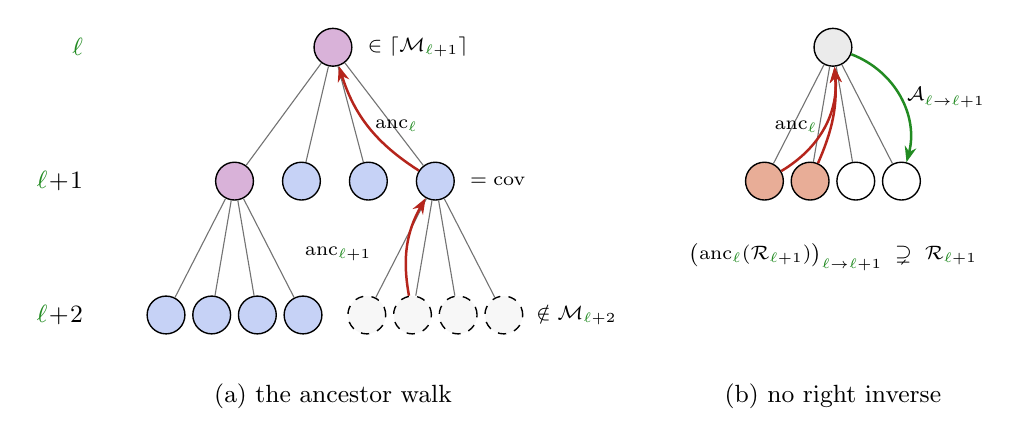
\begin{tikzpicture}[
    >={Stealth[length=2mm]},
    inM/.style   = {draw, circle, minimum size=4.8mm, inner sep=0pt, line width=0.5pt},
    refd/.style  = {inM, fill=Purple!30},
    leafn/.style = {inM, fill=RoyalBlue!30},
    outM/.style  = {inM, dashed, fill=black!3},
    tedge/.style = {draw=black!55, line width=0.4pt},
    walk/.style  = {->, line width=0.9pt, draw=BrickRed},
    back/.style  = {->, line width=0.9pt, draw=ForestGreen},
    lvl/.style   = {font=\small, anchor=east},
    tag/.style   = {font=\scriptsize, inner sep=1pt},
    ttl/.style   = {font=\small, anchor=north}
]

\def\rowA{0}  \def\rowB{-1.7}  \def\rowC{-3.4}
\def\dxC{0.58}
\def\sibA{-3.2} \def\sibB{-0.65}
\def\insx{4.4}

% ---------- level labels, shared by both panels -----------------------
\node[lvl] at (-5.0, \rowA) {$\l$};
\node[lvl] at (-5.0, \rowB) {$\l \! + \! 1$};
\node[lvl] at (-5.0, \rowC) {$\l \! + \! 2$};

% ================= left panel: the ancestor walk ======================
\node[refd] (r) at (-1.95, \rowA) {};

% four siblings, complete because M_{l+1} is quadrisection-closed
\node[refd]  (c1) at (\sibA, \rowB) {};
\node[leafn] (c2) at (-2.35, \rowB) {};
\node[leafn] (c3) at (-1.5, \rowB) {};
\node[leafn] (c4) at (\sibB, \rowB) {};
\foreach \c in {c1,c2,c3,c4} { \draw[tedge] (r) -- (\c); }

% children of c1 are leaves of the forest; children of the leaf c4 exist
% in T_{l+2} but not in M_{l+2}
\foreach \i/\n in {-1.5/g1, -0.5/g2, 0.5/g3, 1.5/g4} {
    \node[leafn] (\n) at ({\sibA + \i*\dxC}, \rowC) {};
    \draw[tedge] (c1) -- (\n);
}
\foreach \i/\n in {-1.5/h1, -0.5/h2, 0.5/h3, 1.5/h4} {
    \node[outM] (\n) at ({\sibB + \i*\dxC}, \rowC) {};
    \draw[tedge] (c4) -- (\n);
}

\draw[walk] (h2) to[bend left=20] (c4);
% label parked in the gap between the two level-(l+2) clusters, since an
% on-path label collides with the dashed nodes
\node[tag, anchor=east] at (-1.42, -2.62) {$\anc{\l+1}$};
\draw[walk] (c4) to[bend left=20] node[tag, right=1pt] {$\anc{\l}$} (r);

% short regime tags at the nodes; the caption carries the full reading
\node[tag, anchor=west] at ($(r.east) + (0.15,0)$) {$\in \ancestorPatch{\M_{\l+1}}$};
\node[tag, anchor=west] at ($(c4.east) + (0.15,0)$) {$= \coveringFace$};
\node[tag, anchor=west] at ($(h4.east) + (0.12,0)$) {$\notin \M_{\l+2}$};
\node[ttl] at (-1.95, -4.15) {(a) the ancestor walk};

% ================= right panel: no right inverse ======================
\node[inM, fill=black!8] (p) at (\insx, \rowA) {};
\node[inM, fill=BrickRed!30] (q1) at ({\insx - 1.5*\dxC}, \rowB) {};
\node[inM, fill=BrickRed!30] (q2) at ({\insx - 0.5*\dxC}, \rowB) {};
\node[inM]                   (q3) at ({\insx + 0.5*\dxC}, \rowB) {};
\node[inM]                   (q4) at ({\insx + 1.5*\dxC}, \rowB) {};
\foreach \n in {q1,q2,q3,q4} { \draw[tedge] (p) -- (\n); }

\draw[walk] (q1) to[bend right=32] node[tag, left=1pt] {$\anc{\l}$} (p);
\draw[walk] (q2) to[bend right=14] (p);
\draw[back] (p) to[bend left=42] node[tag, right=1pt] {$\Aop{}{\l}{\l+1}$} (q4);
\node[tag, anchor=north, align=center] at (\insx, -2.45)
      {$\big( \anc{\l}(\R_{\l+1}) \big)_{\l \to \l+1} \; \supsetneq \; \R_{\l+1}$};
\node[ttl] at (\insx, -4.15) {(b) no right inverse};

\end{tikzpicture}
\end{center}
\caption{\robert{Corollary~\ref{cor:ancestor_walk} read on the quadtree of the faces, the representation of a domain sequence in which Definition~\ref{def:leaf_faces} becomes literal: solid nodes are the faces of the region $\M_\l$ of their level, dashed nodes are faces that exist in the uniform mesh $\T_\l$ but that the domain sequence does not reach, and a leaf face is a solid node without children. Purple marks a face refined beyond its own level, that is an interior node of the tree, and blue marks a leaf. In~(a) the four children of a node are always present together, because $\M_{\l+1}$ is quadrisection-closed, and the red arrows follow the ancestor walk of one face the domain sequence does not reach. The walk meets the three regimes of~\eqref{eq:ancestor_walk} in order, and what Lemma~\ref{lemma:ancestral_closure} forbids is visible as the absence of a fourth: no dashed node lies above a solid one anywhere, so the covering face is a single frontier rather than one of several crossings. In~(b) the same tree shows why $\anc{\l}$ is a left inverse of quadrisection and not a right one. Taking the ancestor of the two red faces and refining again returns all four siblings, so the composition enlarges any region that is not quadrisection-closed. That is the hypothesis $\ancestorPatch{\cdot}$ of Definition~\ref{def:ancestor_patch} carries in its notation and that $\anc{\l}$ does without.}}
\label{fig:ancestor_walk}
\end{figure}

Read from the fine end, the ancestors of a single face therefore pass through three regimes, and the two results above are exactly what forbids a fourth. We first walk the whole hierarchy, starting from the finest level $\L$, where the crossing between the regimes always exists. Afterwards we ask what survives of the split when the walk starts at a coarser level instead.

\begin{lemma}[The ancestor walk at the finest level]
    \label{lemma:ancestor_walk_finest}
    Let $\domseq[\L] \in \alldomseqs_\L$ with regions $\M_\l$ and let $\face{\L}{\fineIdxone} \in \F_\L(\T_\L)$ be a face of the finest mesh. Then $\face{\L}{\fineIdxone}$ has exactly one ancestor that is a leaf face of $\domseq[\L]$, namely its covering face
    \begin{equation}
        \label{eq:covering_face_at_finest}
        \coveringFace \big( \face{\L}{\fineIdxone} \big) \; = \; \anc{\lstar} \big( \face{\L}{\fineIdxone} \big) \; \in \; \leafF{\lstar}(\domseq[\L]) \qquad \text{on a level} \qquad \lzero \leq \lstar \leq \L ,
    \end{equation}
    and its ancestors split by level into
    \begin{equation}
        \label{eq:ancestor_walk}
        \anc{\l} \big( \face{\L}{\fineIdxone} \big) \; \begin{cases}
            \notin \; \M_\l & \text{for} \quad \lzero \leq \lstar < \l \leq \L , \\[2pt]
            \in \; \leafF{\lstar}(\domseq[\L]) & \text{for} \quad \lzero \leq \lstar = \l \leq \L , \\[2pt]
            \in \; \ancestorPatch{\M_{\l+1}} \subseteq \M_{\l} & \text{for} \quad \lzero \leq \l < \lstar \leq \L .
        \end{cases}
    \end{equation}
\end{lemma}
\begin{proof}
    Write $f_\l \coloneq \anc{\l}(\face{\L}{\fineIdxone})$ for the ancestor on level $\l$ and collect the levels on which the walk is inside the domain sequence,
    \begin{equation*}
        S \; \coloneq \; \big\{ \, \lzero \leq \l \leq \L \; \colon \;\; f_\l \in \M_\l \, \big\} .
    \end{equation*}
    The region $\M_\lzero = \F_\lzero(\T_\lzero)$ contains every level-$\lzero$ face by Definition~\ref{def:domseq}, so $\lzero \in S$ and $\lstar \coloneq \max (S)$ exists. Three steps show that this level carries the unique leaf ancestor, which is the assertion.

    \emph{Step 1. $S = \{ \lzero, \, \dots, \, \lstar \}$ is an interval.} Take any $\l < \lstar$. Lemma~\ref{lemma:ancestral_closure} applied to $\{ f_\lstar \} \subseteq \M_\lstar$ places $f_\l$ in $\ancestorPatch{\M_{\l+1}} \subseteq \M_\l$, so $\l \in S$. Above $\lstar$ the definition of the maximum gives $f_\l \notin \M_\l$. These are the third and the first row of~\eqref{eq:ancestor_walk}.

    \emph{Step 2. The ancestor $f_\lstar$ is a leaf face.} Suppose it is not. It lies in $\M_\lstar$, so the splitting~\eqref{eq:leaf_ancestor_split} puts it in $\ancestorPatch{\M_{\lstar+1}}$ and all four of its children lie in $\M_{\lstar+1}$. Were $\lstar$ smaller than $\L$, one of those children would be $f_{\lstar+1}$, which puts $\lstar \! + \! 1$ into $S$ and contradicts maximality. Hence $\lstar = \L$ and $f_\L \in \ancestorPatch{\M_{\L+1}}$, which is empty because Definition~\ref{def:domseq} sets $\M_{\L+1} = \varnothing$. This is the second row of~\eqref{eq:ancestor_walk}, and it is the only step that uses the finest level.

    \emph{Step 3. No other ancestor is a leaf face.} A leaf face lies in the region of its level by Definition~\ref{def:leaf_faces}, which rules out every level above $\lstar$ by Step~1. Below $\lstar$ the ancestor lies in $\ancestorPatch{\M_{\l+1}}$, and~\eqref{eq:leaf_ancestor_split} makes that half of $\M_\l$ disjoint from $\leafF{\l}(\domseq[\L])$.

    Steps~2 and~3 together with Definition~\ref{def:covering_face} give~\eqref{eq:covering_face_at_finest}, and all three steps give~\eqref{eq:ancestor_walk}.
\end{proof}

Lemma~\ref{lemma:ancestor_walk_finest} implies that the escape clause $\coveringFace(\face{\lone}{\fineIdxone}) \coloneq \varnothing$ of Definition~\ref{def:covering_face} cannot fire at the finest level $\L$. This is the one level at which the covering face is always defined, and it is why the constructions below read a neighbourhood at level $\L$ and not at the level of the vertex. Starting the walk from a coarser face on level $\lone$ may or may not cross $\lstar$ as the next corollary shows.

\begin{corollary}[The ancestor walk from a coarser level]
    \label{cor:ancestor_walk}
    Let $\domseq[\L] \in \alldomseqs_\L$ with regions $\M_\l$ and let $\face{\lone}{\fineIdxone} \in \F_\lone(\T_\lone)$ with $\lzero \leq \lone \leq \L$. It holds that
    \begin{itemize}
        \item if $\face{\lone}{\fineIdxone} \notin \ancestorPatch{\M_{\lone+1}}$, i.e. it is not refined beyond level $\lone$, then
        \begin{itemize}
            \item[$(i)$] $\face{\lone}{\fineIdxone}$ has exactly one ancestor $\anc{\lstar}(\face{\lone}{\fineIdxone}) = \coveringFace(\face{\lone}{\fineIdxone}) \in \leafF{\lstar}(\domseq[\L])$ on a level $\lzero \leq \lstar \leq \lone$ that is also a leaf face,
            \item[$(ii)$] and its ancestors $\anc{\l}(\face{\lone}{\fineIdxone})$ split by level as in~\eqref{eq:ancestor_walk}, with $\L$ replaced by $\lone$ throughout;
        \end{itemize}
        \item if $\face{\lone}{\fineIdxone} \in \ancestorPatch{\M_{\lone+1}}$, i.e. it is refined beyond level $\lone$, then
        \begin{itemize}
            \item[$(i')$] $\face{\lone}{\fineIdxone}$ has no covering face, i.e. $\coveringFace(\face{\lone}{\fineIdxone}) = \varnothing$,
            \item[$(ii')$] and $\anc{\l}(\face{\lone}{\fineIdxone}) \in \ancestorPatch{\M_{\l+1}} \subseteq \M_\l$ for all $\lzero \leq \l \leq \lone$.
        \end{itemize}
    \end{itemize}
\end{corollary}
\begin{proof}
    Pick any descendant $\face{\L}{\fineIdxtwo} \in \Aop{}{\lone}{\L}(\face{\lone}{\fineIdxone})$ on the finest level and let $\lstar$ be the level that Lemma~\ref{lemma:ancestor_walk_finest} gives for it. Ancestry composes, so $\anc{\l}(\face{\lone}{\fineIdxone}) = \anc{\l}(\face{\L}{\fineIdxtwo})$ for all $\lzero \leq \l \leq \lone$ and the walk of $\face{\lone}{\fineIdxone}$ is the tail of the walk of $\face{\L}{\fineIdxtwo}$. Everything follows from whether that tail still reaches the crossing at $\lstar$.

    \emph{The tail reaches it exactly when $\face{\lone}{\fineIdxone} \notin \ancestorPatch{\M_{\lone+1}}$.} Read~\eqref{eq:ancestor_walk} at $\l = \lone$. Its third row is the condition $\lone < \lstar$ and places $\face{\lone}{\fineIdxone}$ in $\ancestorPatch{\M_{\lone+1}}$. The other two rows place it outside $\M_\lone$ or inside $\leafF{\lone}(\domseq[\L])$, and the nesting condition of Definition~\ref{def:domseq} and the splitting~\eqref{eq:leaf_ancestor_split} keep both apart from $\ancestorPatch{\M_{\lone+1}}$. The rows are exhaustive, so $\lstar > \lone$ holds exactly when $\face{\lone}{\fineIdxone}$ is refined beyond its own level.

    \emph{The surviving branch.} Let $\lstar \leq \lone$. The tail carries all three rows of~\eqref{eq:ancestor_walk} over the range $\lzero \leq \l \leq \lone$, which is~$(ii)$. It also contains the level $\lstar$, so it inherits the leaf ancestor of the lemma together with its uniqueness, and Definition~\ref{def:covering_face} names that ancestor the covering face. That is~$(i)$.

    \emph{The dying branch.} Let $\lstar > \lone$. Every level of the tail falls in the third row of~\eqref{eq:ancestor_walk}, which is~$(ii')$. The one leaf ancestor sits at $\lstar$ and thus outside the tail, so the walk from $\lone$ meets none and $\coveringFace(\face{\lone}{\fineIdxone}) = \varnothing$ by Definition~\ref{def:covering_face}, which is~$(i')$.

    Neither branch depends on the descendant we picked. The branch is fixed by the hypothesis through the equivalence above, and $\lstar$ is then fixed by the uniqueness in~$(i)$.
\end{proof}

\robert{Figure~\ref{fig:ancestor_walk} draws the two results on the quadtree of the faces rather than on the mesh, which is where their content lives. The trichotomy is a statement about ancestry, and ancestry is the tree.}

\medskip

The rest of this section reads a vertex on more than one level, so we now fix what it means to speak of a vertex across the hierarchy. Loop subdivision retains every vertex of $\T_\l$ as a vertex of $\T_{\l+1}$ and inserts one new vertex per edge, see Section~\ref{subsec:subdiv_basis_functions}. This gives an injection
\begin{equation}
    \label{eq:vertex_injection}
    \V_\l(\T_\l) \; \hookrightarrow \; \V_{\l+1}(\T_{\l+1}) , \qquad \vertex{\l}{\coarseIdxone} \; \longmapsto \; \vertex{\l+1}{\coarseIdxone} ,
\end{equation}
whose complement is precisely the set of vertices inserted on level $\l \! + \! 1$. This is the action of $\Aop{}{\l}{\lone}$ on vertices used in Section~\ref{subsec:selecting_active_dofs}, and unlike its action on faces it is single-valued: a face has four children, a vertex has one image. The identification is combinatorial and not geometric, since subdivision moves the position of a vertex on every level.

\begin{definition}[Vertex class and birth level]
    \label{def:vertex_class}
    Call two vertices of the hierarchy \emph{equivalent} when one is carried onto the other by a composition of the injections~\eqref{eq:vertex_injection}. A \emph{vertex class} $\vertexClass{\coarseIdxone}$ is an equivalence class of this relation, that is the orbit of a single vertex under refinement. Its \emph{birth level} $\birthLevel(\vertexClass{\coarseIdxone})$ is the coarsest level carrying a representative so that
    \begin{equation}
        \label{eq:vertex_class}
        \vertexClass{\coarseIdxone} \; = \; \big\{ \vertex{\lone}{\coarseIdxone} \; \colon \;\; \birthLevel(\vertexClass{\coarseIdxone}) \, \leq \, \lone \, \leq \, \L \big\} ,
    \end{equation}
    and we write $\vertex{\lone}{\coarseIdxone}$ for the representative of $\vertexClass{\coarseIdxone}$ on level $\lone$, which exists exactly for $\lone \geq \birthLevel(\vertexClass{\coarseIdxone})$. We denote the set of all vertex classes of a mesh hierarchy by $\vertexClasses$.
\end{definition}

Every class has one representative on each level from its birth level up to $\L$ and none below. The classes of birth level $\lzero$ are the vertices of the control mesh, and a class of birth level $\l > \lzero$ is the vertex that the quadrisection of level $\l \! - \! 1$ inserts on one of its edges.

The number of vertex classes $\vertexClasses$ is exactly the number of vertices of level $\L$ because every vertex $\vertex{\L}{\coarseIdxone}$ is a representative of its vertex class $\vertexClass{\coarseIdxone}$. For that reason, we will often state properties and operators on $\vertexClasses$ in terms of $\vertex{\L}{\coarseIdxone}$.

\begin{definition}[Class star]
    \label{def:star_ancestry}
    Let $\vertexClass{\coarseIdxone} \in \vertexClasses$ be a vertex class with level-$L$ representative $\vertex{\L}{\coarseIdxone}$ and let $\l \in \{ \lzero, \, \dots, \, \L \}$. The \emph{class star} of $\vertexClass{\coarseIdxone}$ on level $\l$ is the set
    \begin{equation}
        \label{eq:star_ancestry}
        \FVanc{\l} \big( \vertexClass{\coarseIdxone} \big) \; \coloneq \; \anc{\l} \big( \FVl{\L} ( \vertex{\L}{\coarseIdxone} ) \big)
    \end{equation}
    of those level-$\l$ faces that have a child in the mesh star $\FVl{\L}(\vertex{\L}{\coarseIdxone})$ of $\vertex{\L}{\coarseIdxone}$.
\end{definition}

On the levels $\l \geq \birthLevel(\vertexClass{\coarseIdxone})$ at which the class representative $\vertex{\l}{\coarseIdxone}$ exists, the class star coincides with the mesh star, i.e.
\begin{equation}
    \label{eq:star_ancestry_is_star}
    \FVanc{\l} \big( \vertexClass{\coarseIdxone} \big) \; = \; \FVl{\l} \big( \vertex{\l}{\coarseIdxone} \big), \qquad \l \geq \birthLevel(\vertexClass{\coarseIdxone}),
\end{equation}
What the star ancestry adds are the coarser levels $\l < \birthLevel(\vertexClass{\coarseIdxone})$, at which $\vertexClass{\coarseIdxone}$ has no representative and $\FVl{\l}$ is undefined. For Loop subdivision, the class star on level $\birthLevel(\vertexClass{\coarseIdxone}) \! - \! 1$ contains the two faces sharing the edge on which $\vertex{\birthLevel(\vertexClass{\coarseIdxone})}{\coarseIdxone}$ will be created. On the levels below $\birthLevel(\vertexClass{\coarseIdxone}) \! - \! 1$, the class star contains the ancestors of those two faces, which may coincide in a single face. Thus, the class star satisfies the following nestedness property:
\begin{equation}
    \label{eq:star_ancestry_nested}
    \FVanc{\l+1} ( \vertexClass{\coarseIdxone} ) \; \subseteq \; \Aop{}{\l}{\l+1} \big( \FVanc{\l} ( \vertexClass{\coarseIdxone} ) \big) \qquad \text{for} \qquad \lzero \leq \l < \L.
\end{equation}

\begin{definition}[Leaf star]
    \label{def:leaf_star}
    Let $\domseq[\L] \in \alldomseqs_\L$ and let $\vertexClass{\coarseIdxone} \in \vertexClasses(\T_\L)$ be a vertex class with finest representative $\vertex{\L}{\coarseIdxone}$. The \emph{leaf star} $\FVleaf{} \big( \vertexClass{\coarseIdxone} \big)$ is the collection of all leaf faces of $\domseq[\L]$ covering the mesh star $\FVl{\L}(\vertex{\L}{\coarseIdxone})$, i.e.
    \begin{equation}
        \label{eq:leaf_star}
        \FVleaf{} \big( \vertexClass{\coarseIdxone} \big) \; \coloneq \; \big\{ \coveringFace \big( \face{\L}{\fineIdxone} \big) \; \colon \;\; \face{\L}{\fineIdxone} \in \FVl{\L} \big( \vertex{\L}{\coarseIdxone} \big) \big\}.
    \end{equation}
    Note that the covering face exists for every $\face{\L}{\fineIdxone}$ because of Equation~\eqref{eq:covering_face_at_finest}. We add a level subscript to the leaf star to indicate its \emph{level-$\l$ slice}
    \begin{equation}
        \label{eq:leaf_star_slice}
        \FVleaf{\l} ( \vertexClass{\coarseIdxone} ) \; \coloneq \; \FVleaf{} ( \vertexClass{\coarseIdxone} ) \cap \F_\l(\T_\l) \;\; \subseteq \;\; \leafF{\l}(\domseq[\L]).
    \end{equation}
\end{definition}

The class star of Definition~\ref{def:star_ancestry} and the leaf star of Definition~\ref{def:leaf_star} are therefore the same construction reading two different ways to move across the hierarchy. Both start from the mesh star $\FVl{\L}(\vertex{\L}{\coarseIdxone})$ at the finest level. The class star climbs uniformly to a prescribed level $\l$ using the ancestor operator $\anc{\l}$ of Definition~\ref{def:face_ancestor}. In contrast, the leaf star collects the leaf faces covering the mesh star at whichever level the domain sequence happens them and is thus fully determined by the domain sequence.

% --- Figure knobs: one vertex read at every level. Generated by
% plot_leaf_star_duality.py in the subdiv_FE repo from input_partition.vtk and
% input_level_meshes.vtk of padding_output/v8_graded_top_bottom_sides -- the
% same domain sequence, and the same marked vertex, as
% Figure~\ref{fig:pinch_single_arc}, so the purple in that panel is this
% vertex's refinement fan at level 0. The second file exists for this figure:
% the leaf mesh alone carries neither the level-$\l$ faces inside a coarse leaf
% nor the level-$\l$ face a refined region descends from, and both are drawn
% here. No panel is zoomed, so all four show the same domain at the same scale
% and the shrinking star is read against a fixed frame. The first panel is
% narrower only because its generated aspect ratio differs, so that the four
% come out the same height. Reuses \cvsubfig from
% Section~\ref{subsec:subdiv_partition}.
% The panels are generated in the orientation the solver writes them and are
% turned a quarter turn anticlockwise here, so that regenerating them does not
% undo the rotation. \cvsubfigrot is \cvsubfig with that rotation applied
% before the width is fit, so #1 is still the panel width on the page. The
% width fractions are those of the rotated panels: the three level panels are
% square, the overview is 110.574 x 109.041 pt before rotation and so is fit
% slightly wider than they are, to come out at the same height.
\newcommand{\cvsubfigrot}[4][\cvScale]{% #1 width fraction  #2 image path  #3 caption  #4 label
    \begin{subfigure}[t]{#1\textwidth}
        \centering
        \includegraphics[angle=90,width=\textwidth]{#2}
        \caption{#3}
        \label{#4}
    \end{subfigure}%
}
\begin{figure}[tb]
    \centering
    \cvsubfigrot[0.2383]
        {images/visualisations/v8_graded_top_bottom_sides_leafstar_overview.pdf}
        {The leaf mesh of $\domseq[2]$ and the query vertex $\vertex{2}{\coarseIdxone}$ (yellow).}
        {fig:leafstar_overview}
    \hfill
    \cvsubfigrot[0.235]
        {images/visualisations/v8_graded_top_bottom_sides_leafstar_lvl0.pdf}
        {$\l = \lzero$: six of the eight star faces are refined beyond level $\lzero$, two are leaf faces.}
        {fig:leafstar_l0}
    \hfill
    \cvsubfigrot[0.235]
        {images/visualisations/v8_graded_top_bottom_sides_leafstar_lvl1.pdf}
        {$\l = 1$: two faces refined beyond level $1$, four leaf faces on level $1$, two from level $\lzero$.}
        {fig:leafstar_l1}
    \hfill
    \cvsubfigrot[0.235]
        {images/visualisations/v8_graded_top_bottom_sides_leafstar_lvl2.pdf}
        {$\l = 2$: no faces refined beyond level $2$, so the leaf star covers the whole mesh star.}
        {fig:leafstar_l2}
    \caption{Decomposition of the mesh stars of the yellow vertex across levels $\lzero$, $1$, and $2$ according to Equation~\eqref{eq:star_splits}. Panels~\subref{fig:leafstar_l0} to~\subref{fig:leafstar_l2} show the whole uniform mesh $\T_\l$ of its level, with the eight faces of the mesh star $\FVl{\l}$ of the yellow vertex outlined. The refinement fan $\refFan{\l}$ is purple, the leaf star $\FVleaf{}$ is blue with each of its leaf faces outlined so that they can be identified across levels. Reading across, the refinement fan empties while the leaf star fills, and the first level at which nothing is refined beyond it is $\lmax = 2$, where the leaf star covers the mesh star with faces from levels $\lzero$, $1$ and $2$ together.}
    \label{fig:leaf_star_levels}
\end{figure}

By Definition~\ref{def:leaf_star}, a leaf face of the leaf star covers a face of $\FVl{\L}(\vertex{\L}{\coarseIdxone})$ and thus it holds that
\begin{equation}
    \label{eq:leaf_star_in_ancestry}
    \FVleaf{\l} \big( \vertexClass{\coarseIdxone} \big) \; \subseteq \; \FVanc{\l} \big( \vertexClass{\coarseIdxone} \big).
\end{equation}

Fix a vertex class $\vertexClass{\coarseIdxone}$ and a level $\l \geq \birthLevel(\vertexClass{\coarseIdxone})$, so that the class has a representative $\vertex{\l}{\coarseIdxone}$ on that level. Corollary~\ref{cor:ancestor_walk} applies to a face of the mesh star $\FVl{\l}(\vertex{\l}{\coarseIdxone})$ read at level $\l$. It gives either no covering face or exactly one, on a level $\lstar \leq \l$. Three cases follow. A face with no covering face is refined beyond $\l$ and lies in the refinement fan $\refFan{\l}(\vertex{\l}{\coarseIdxone})$. A face with $\lstar = \l$ is its own covering face and lies in the slice $\FVleaf{\l}(\vertexClass{\coarseIdxone})$. A face with $\lstar < \l$ descends from a coarser leaf face in $\FVleaf{\lstar}(\vertexClass{\coarseIdxone})$. The three cases are exhaustive and disjoint because $\lstar$ is unique whenever it exists. Removing the third case leaves the first two, that is
\begin{equation}
    \label{eq:star_splits}
    \FVl{\l}(\vertex{\l}{\coarseIdxone}) \, \setminus \, \bigsqcup\limits_{\lstar = \lzero}^{\l-1} \; \Aop{}{\lstar}{\l} \, \big( \FVleaf{\lstar} (\vertexClass{\coarseIdxone}) \big) \; = \; \refFan{\l} \big( \vertex{\l}{\coarseIdxone} \big) \; \sqcup \;  \FVleaf{\l} \big( \vertexClass{\coarseIdxone} \big) \qquad \forall \l \; \geq \; \birthLevel(\vertexClass{\coarseIdxone}) .
\end{equation}

Figure~\ref{fig:leaf_star_levels} follows a single vertex class through~\eqref{eq:star_splits}. Read across the row the refinement fan turns into the leaf star level by level by splitting off the level-$\l$ slice $\FVleaf{\l} ( \vertexClass{\coarseIdxone} )$.

\begin{definition}[Coarsest and finest level of a leaf star]
    \label{def:level_range}
    Let $\FVleaf{}(\vertexClass{\coarseIdxone})$ be the leaf star of the vertex class $\vertexClass{\coarseIdxone}$. We write
    \begin{alignat}{2}
        \label{eq:level_range}
        \lminIdx{\coarseIdxone} &= \lmin ( \vertexClass{\coarseIdxone} ) &&\coloneq \min \{ \l \; \colon \; \FVleaf{\l}(\vertexClass{\coarseIdxone}) \cap \F_\l(\T_\l) \neq \varnothing \}, \\
        \lmaxIdx{\coarseIdxone} &= \lmax ( \vertexClass{\coarseIdxone} ) &&\coloneq \max \{ \l \; \colon \; \FVleaf{\l}(\vertexClass{\coarseIdxone}) \cap \F_\l(\T_\l) \neq \varnothing \}
    \end{alignat}
    for the coarsest and the finest level of faces contained in the leaf star of $\vertexClass{\coarseIdxone}$. Finally, we define the \emph{level span} $\mu_\coarseIdxone$ of the leaf star by $\levelSpan{\coarseIdxone} \coloneq \lmaxIdx{\coarseIdxone} - \lminIdx{\coarseIdxone}$.
\end{definition}

\subsection{Refinement operators}
\label{subsec:refinement_operators}
\label{subsec:operations_on_coverings}

The remainder of this section introduces operators that enable the kinds of refinement that we will later need for the adaptive loop in Section~\ref{subsec:adaptive_loop}. The \emph{face quadrisection operator} $\quadriF(\domseq[\L], \simplexsubset{2}{})$ refines a set of faces $\simplexsubset{2}{}$, given one level at a time, by adding their children to the next level of the domain sequence and leaving everything else untouched.

\begin{definition}[Face quadrisection operator]
    \label{def:face_quadrisection_operator}
    Let $\domseq[\L] \in \alldomseqs$ be a domain sequence with regions $\M_\l$, $\l \in \{ \lzero, \, \dots \,, \L\}$, and let $\simplexsubset{2}{}$ be a set of faces of $\domseq[\L]$ given by
    \begin{equation}
        \label{eq:marked_face_family}
        \simplexsubset{2}{} \; \subseteq \bigsqcup\limits_{\l = \lzero}^{\L-1} \M_\l \quad \text{and} \quad \simplexsubset{2}{\l} \; \coloneq \; \simplexsubset{2}{} \cap \M_\l.
    \end{equation}
    The \emph{face quadrisection operator} $\quadriF \; \colon \; \alldomseqs \times \powerset \big( \bigsqcup_{\l = \lzero}^{\L-1} \M_\l \big) \; \longrightarrow \; \alldomseqs$ is defined levelwise by
    \begin{equation}
        \label{eq:def_face_quadrisection_operator}
        \quadriF \big( \domseq[\L], \, \simplexsubset{2}{} \big) \; \coloneq \; \M_\lzero \, \sqcup \; \bigsqcup\limits_{\l = \lzero}^{\L-1} \, \big( \M_{\l+1} \, \cup \, \Aop{}{\l}{\l+1}(\simplexsubset{2}{\l}) \big).
    \end{equation}
    We keep writing $\quadriF ( \domseq[\L], \simplexsubset{2}{\l} )$ if $\simplexsubset{2}{}$ is a single-level $\l$ set of faces.
\end{definition}

The result is again a domain sequence because each added set is quadrisection-closed with ancestor $\simplexsubset{2}{\l}$, and so is a union of such sets. The nesting condition of Definition~\ref{def:domseq} holds because $\ancestorPatch{\M_{\l+1} \cup \Aop{}{\l}{\l+1}(\simplexsubset{2}{\l})} = \ancestorPatch{\M_{\l+1}} \cup \simplexsubset{2}{\l} \subseteq \M_\l$ because the slices of $\simplexsubset{2}{}$ are subsets of the regions by~\eqref{eq:marked_face_family}. Note further that if $\simplexsubset{2}{\l} \subseteq \ancestorPatch{\M_{\l+1}}$ on every level $\l$, then $\quadriF ( \domseq[\L], \simplexsubset{2}{} ) = \domseq[\L]$ is the identity, because all marked faces already are refined beyond their level in the domain sequence.

\smallskip

The refinement and padding steps of the adaptive loop in Section~\ref{subsec:adaptive_loop} iterate over the vertices $\V(\domseq[\L])$ of the domain sequence $\domseq[\L]$ defined in Equation~\eqref{eq:vertices_of_domseq}. This is the set of vertices on which the following refinement operators are defined. Recall that Equation~\eqref{eq:vertices_of_domseq} takes the disjoint union over the levels, so an element of $\V(\domseq[\L])$ is a vertex \emph{together with} a level at which it exists, and a subset of $\V(\domseq[\L])$ may carry the same vertex on several levels.

The remaining refinement operator raises a whole neighbourhood of a vertex to a prescribed target level. In spirit it adds the mesh star of the vertex on every level up to that target, which is what makes it close a pinch, cf.\ Lemma~\ref{lemma:pinch_spent}. On the levels coarser than the one the vertex is born on, where the vertex is not a mesh vertex and has no mesh star, the star ancestry $\FVanc{\lone}$ of Definition~\ref{def:star_ancestry} takes its place.

Whether a star ancestry has to be added at all is decided by the leaf star, and the following lemma is the one place where the two meet. \robert{It locates the sharp threshold: below the coarsest level of the leaf star the star ancestry is not merely present in the domain sequence, it is already refined beyond its level, and at that coarsest level it stops being so.}

\begin{lemma}[Absorption of the star ancestry]
    \label{lemma:ancestry_absorbed}
    Let $\domseq[\L] \in \alldomseqs$ with regions $\M_\lone$, let $\vertex{\l}{\coarseIdxone} \in \V(\domseq[\L])$ with leaf star $\FVleaf{}(\vertex{\l}{\coarseIdxone})$ of coarsest level $\lmin$. Then every face of the star ancestry below $\lmin$ is refined beyond its own level,
    \begin{equation}
        \label{eq:ancestry_absorbed}
        \FVanc{\lone} \big( \vertex{\l}{\coarseIdxone} \big) \; \subseteq \; \ancestorPatch{\M_{\lone+1}} \qquad \text{for all} \qquad \lzero \leq \lone < \lmin,
    \end{equation}
    and consequently the domain sequence already contains all children of that star ancestry,
    \begin{equation}
        \label{eq:ancestry_absorbed_children}
        \Aop{}{\lone}{\lone+1} \Big( \FVanc{\lone} \big( \vertex{\l}{\coarseIdxone} \big) \Big) \; \subseteq \; \M_{\lone+1} \qquad \text{for all} \qquad \lzero \leq \lone < \lmin.
    \end{equation}
    Both fail the first time at $\lone = \lmin$.
\end{lemma}
\begin{proof}
    \robert{Let $\lone < \lmin$ and let $\face{\lone}{\fineIdxone} \in \FVanc{\lone}(\vertex{\l}{\coarseIdxone})$. By Definition~\ref{def:star_ancestry} it is $\anc{\lone}(\face{\L}{\fineIdxtwo})$ for some $\face{\L}{\fineIdxtwo} \in \FVl{\L}(\vertex{\L}{\coarseIdxone})$, so Lemma~\ref{lemma:ancestor_walk_finest} applies to $\face{\L}{\fineIdxtwo}$. Its covering face lies in the leaf star by Definition~\ref{def:leaf_star}, so the level $\lstar$ of that covering face satisfies $\lstar \geq \lmin > \lone$. This is the only place at which the hypothesis $\lone < \lmin$ enters. The third row of~\eqref{eq:ancestor_walk} read at $\l = \lone$ is then~\eqref{eq:ancestry_absorbed}, and a face of $\ancestorPatch{\M_{\lone+1}}$ has all four of its children in $\M_{\lone+1}$, which is~\eqref{eq:ancestry_absorbed_children}.

    At $\lone = \lmin$ both inclusions genuinely fail. The slice $\FVleaf{\lmin}(\vertex{\l}{\coarseIdxone})$ is non-empty by the definition of $\lmin$ and contained in $\FVanc{\lmin}(\vertex{\l}{\coarseIdxone})$ by~\eqref{eq:leaf_star_in_ancestry}. Any of its faces is a leaf face, so it lies outside $\ancestorPatch{\M_{\lmin+1}}$ by Definition~\ref{def:leaf_faces} and no descendant of it lies in $\M_{\lmin+1}$ by Corollary~\ref{cor:leaf_faces_terminal}. These are the two failures.}
\end{proof}

\robert{Since the star ancestry is fixed by the vertex and the uniform meshes, several vertices can be raised at once by taking the union, and no order has to be fixed. This is the form in which Section~\ref{subsec:adaptive_loop} uses the operator: each of its steps supplies a set of vertices and a target level for each of them.}

\begin{definition}[Graded vertex quadrisection operator]
    \label{def:graded_vertex_quadrisection}
    Let $\domseq[\L] \in \alldomseqs$ with regions $\M_\l$, let $W \subseteq \V(\domseq[\L])$ be a set of vertices of the domain sequence, and let $\targetlevel \colon W \to \{ \lzero, \, \dots, \, \L \}$ assign a target level to each of them. The \emph{graded vertex quadrisection operator}
    \begin{equation}
        \quadriVup{\targetlevel} \; \colon \; \alldomseqs \times \powerset\big( \V(\domseq[\L]) \big) \; \longrightarrow \; \alldomseqs
    \end{equation}
    is defined levelwise by
    \begin{equation}
        \label{eq:graded_vertex_quadrisection}
        \quadriVup{\targetlevel} \big( \domseq[\L], \, W \big) \; \coloneq \; \M_\lzero \, \sqcup \bigsqcup\limits_{\lone = \lzero}^{\L-1} \Bigg( \M_{\lone+1} \; \cup \bigcup\limits_{\substack{w \, \in \, W \\ \lone \, < \, \targetlevel(w)}} \Aop{}{\lone}{\lone+1} \big( \FVanc{\lone}(w) \big) \Bigg),
    \end{equation}
    \robert{indexed, like the face quadrisection~\eqref{eq:def_face_quadrisection_operator}, by the level $\lone$ of the faces that are refined.} We write $\quadriVup{t}(\domseq[\L], W)$ when the target level $\targetlevel \equiv t$ is the same for all vertices, and $\quadriVup{\targetlevel}(\domseq[\L], w)$ for a single vertex $W = \{ w \}$.
\end{definition}

\robert{The right-hand side of~\eqref{eq:graded_vertex_quadrisection} is again a domain sequence. Every added set is quadrisection-closed, hence so is every union of them, and the nesting condition of Definition~\ref{def:domseq} follows from~\eqref{eq:star_ancestry_nested},
\begin{equation}
    \ancestorPatch{\tilde{\M}_{\lone+1}} \; = \; \ancestorPatch{\M_{\lone+1}} \cup \bigcup\limits_{\substack{w \, \in \, W \\ \lone \, < \, \targetlevel(w)}} \FVanc{\lone}(w) \; \subseteq \; \M_\lone \cup \bigcup\limits_{\substack{w \, \in \, W \\ \lone - 1 \, < \, \targetlevel(w)}} \Aop{}{\lone-1}{\lone} \big( \FVanc{\lone-1}(w) \big) \; = \; \tilde{\M}_\lone,
\end{equation}
where the index set grows because $\lone < \targetlevel(w)$ implies $\lone \! - \! 1 < \targetlevel(w)$.}

\begin{corollary}[\robert{Vertexwise decomposition of the graded quadrisection}]
    \label{cor:graded_quadrisection_composition}
    \robert{Let $\domseq[\L] \in \alldomseqs$, let $W \subseteq \V(\domseq[\L])$ and $\targetlevel \colon W \to \{ \lzero, \, \dots, \, \L \}$ be as in Definition~\ref{def:graded_vertex_quadrisection}, and let $w_1, \, \dots, \, w_{\vert W \vert}$ be any enumeration of $W$. Then
    \begin{equation}
        \label{eq:graded_quadrisection_composition}
        \quadriVup{\targetlevel} \big( \domseq[\L], \, W \big) \; = \; \domseq[\L]^{\vert W \vert}, \qquad \domseq[\L]^{0} \coloneq \domseq[\L], \qquad \domseq[\L]^{p} \coloneq \quadriVup{\targetlevel(w_p)} \big( \domseq[\L]^{p-1}, \, w_p \big).
    \end{equation}
    In particular the result is independent of the enumeration and the operator is idempotent. Moreover, $\quadriVup{\targetlevel}(\domseq[\L], W) = \domseq[\L]$ is the identity if and only if every $w \in W$ satisfies $\lmin(\FVleaf{}(w)) \geq \targetlevel(w)$ in $\domseq[\L]$.}
\end{corollary}
\begin{proof}
    \robert{Definition~\ref{def:graded_vertex_quadrisection} adjoins to each region the union of sets that depend on the vertex and its target level alone, so both sides of~\eqref{eq:graded_quadrisection_composition} adjoin the same union to $\M_\lone$, and unions are commutative, associative and idempotent. The last assertion compares two thresholds on the same axis. Definition~\ref{def:graded_vertex_quadrisection} adjoins something for $w$ exactly on the levels $\lone < \targetlevel(w)$, and~\eqref{eq:ancestry_absorbed_children} says that what it would adjoin is already there exactly on the levels $\lone < \lmin$. If $\targetlevel(w) \leq \lmin$ for every $w \in W$, the first range is contained in the second and every adjoined set is redundant. If $\lmin < \targetlevel(w)$ for some $w$, then $\lone = \lmin$ lies in the first range but not in the second, so the operator adjoins a child of $\FVanc{\lmin}(w)$ that Lemma~\ref{lemma:ancestry_absorbed} places outside $\M_{\lmin+1}$.}
\end{proof}

\robert{The operator also fixes what the leaf star of the vertex looks like afterwards, which is what the grading step of Section~\ref{subsec:padding} reads off it.}

\begin{corollary}[\robert{Leaf star of the output}]
    \label{cor:graded_quadrisection_leafstar}
    \robert{Let $\domseq[\L] \in \alldomseqs$, let $\vertex{\l}{\coarseIdxone} \in \V(\domseq[\L])$ with leaf star of coarsest level $\lmin$ and finest level $\lmax$, and let $\targetlevel \in \{ \lzero, \, \dots, \, \L \}$. The leaf star of $\vertex{\l}{\coarseIdxone}$ read on $\quadriVup{\targetlevel}(\domseq[\L], \vertex{\l}{\coarseIdxone})$ has
    \begin{equation}
        \label{eq:graded_quadrisection_leafstar}
        \lmin' \; = \; \max \big( \lmin, \, \targetlevel \big) \qquad \text{and} \qquad \lmax' \; = \; \max \big( \lmax, \, \targetlevel \big),
    \end{equation}
    and hence level span $\mu' = \max(\lmax, \targetlevel) - \max(\lmin, \targetlevel)$. In particular $\mu' = \lmax - \targetlevel$ whenever $\lmin < \targetlevel \leq \lmax$. For a set $W \ni \vertex{\l}{\coarseIdxone}$ of vertices the two equalities weaken to $\lmin' \geq \max(\lmin, \targetlevel(\vertex{\l}{\coarseIdxone}))$ and $\lmax' \geq \max(\lmax, \targetlevel(\vertex{\l}{\coarseIdxone}))$, because the other vertices of $W$ may refine into this leaf star as well.}
\end{corollary}
\begin{proof}
    \robert{Write $\vertex{\L}{\coarseIdxone} = \Aop{}{\l}{\L}(\vertex{\l}{\coarseIdxone})$ and let $\tilde{\M}$ denote the regions of the output. If $\lmin \geq \targetlevel$ the operator is the identity by Corollary~\ref{cor:graded_quadrisection_composition} and there is nothing to prove, so let $\lmin < \targetlevel$.

    For every $\lone < \targetlevel$, Definition~\ref{def:graded_vertex_quadrisection} puts $\Aop{}{\lone}{\lone+1}(\FVanc{\lone}(\vertex{\l}{\coarseIdxone}))$ into $\tilde{\M}_{\lone+1}$, so $\FVanc{\lone}(\vertex{\l}{\coarseIdxone}) \subseteq \ancestorPatch{\tilde{\M}_{\lone+1}}$ because $\tilde{\M}_{\lone+1}$ is quadrisection-closed. Each face of $\FVl{\L}(\vertex{\L}{\coarseIdxone})$ has its level-$\lone$ ancestor in $\FVanc{\lone}(\vertex{\l}{\coarseIdxone})$ by Definition~\ref{def:star_ancestry}, so that ancestor is refined beyond $\lone$ and the face is covered on no level below $\targetlevel$. Hence $\lmin' \geq \targetlevel$. Conversely, pick a leaf face $\face{\lmin}{\coarseIdxone} \in \FVleaf{\lmin}(\vertex{\l}{\coarseIdxone})$ of the input. No descendant of it lies in a region of $\domseq[\L]$ by Corollary~\ref{cor:leaf_faces_terminal}, and the operator adjoins faces on no level above $\targetlevel$, so its descendant in $\FVanc{\targetlevel}(\vertex{\l}{\coarseIdxone})$ is a leaf face of the output on level $\targetlevel$ covering a face of the mesh star. Thus $\lmin' = \targetlevel = \max(\lmin, \targetlevel)$.

    For the finest level, the operator refines only faces of the star ancestries on levels $\lone < \targetlevel$, so a leaf face of the input leaf star on a level $\geq \targetlevel$ is untouched and remains one of the output. If $\targetlevel \leq \lmax$, the level-$\lmax$ leaf face survives and nothing finer is added, giving $\lmax' = \lmax$. If $\targetlevel > \lmax$, the previous paragraph lifts every leaf face of the star to $\targetlevel$ and $\lmax' = \targetlevel$. Both cases are $\lmax' = \max(\lmax, \targetlevel)$. The statement for a set follows because the regions only grow when further vertices are added, so no leaf face of the star gets coarser.}
\end{proof}

\guidance{This is what licenses the sentence in the grading paragraph of Section~\ref{subsec:padding} that $\quadriVup{\lmax{}_{,\coarseIdxtwo} - g}$ ``closes the level span to exactly $g$''. With $\targetlevel = \lmax - g$ and $\mu > g$ one has $\lmin < \targetlevel \leq \lmax$, so $\mu' = g$ by~\eqref{eq:graded_quadrisection_leafstar}. Note the caveat in the last sentence of the corollary. Grading refines a whole set of vertices at once, so the span of a graded vertex can come out \emph{below} $g$ if a neighbour's grading reaches into its leaf star. Worth deciding whether the grading paragraph should say ``at most $g$'' rather than ``exactly $g$''.}

\robert{The operator is not evaluated through~\eqref{eq:graded_vertex_quadrisection} in practice. The implementation never forms a star ancestry and works with the leaf star instead, one vertex and one level at a time.}

\begin{remark}[\robert{How the implementation evaluates $\quadriVup{\targetlevel}$}]
    \label{rem:graded_quadrisection_algorithm}
    \robert{Let $\vertex{\l}{\coarseIdxone} \in \V(\domseq[\L])$ be a single vertex with target level $\targetlevel$, and let $\lmin = \lmin(\FVleaf{}(\vertex{\l}{\coarseIdxone}))$ be read on the input $\domseq[\L]$. The implementation grades the leaf star from $\lmin$ to $\targetlevel$ by the iterative refinement algorithm}
    \begin{enumerate}
        \item initialise $\domseq[\L,\lmin] \coloneq \domseq[\L]$,
        \item iterate \robert{$\domseq[\L, \lone + 1] = \quadriF \big( \domseq[\L, \lone], \, \FVleaf{\lone}(\vertex{\l}{\coarseIdxone}) \big)$}, refining the coarsest slice of the leaf star read on $\domseq[\L, \lone]$, for $\lone \in \{ \lmin, \dots, \targetlevel-1 \}$,
        \item \robert{return $\domseq[\L, \targetlevel]$, and return $\domseq[\L]$ unchanged if $\lmin \geq \targetlevel$.}
    \end{enumerate}
    Note that step 2 recomputes the leaf star on every $\domseq[\L,\lone]$ that resulted from refining its coarsest faces on the previous step. This ensures that the refined children of exactly these faces are picked up and refined again until the target level is reached. Figure~\ref{fig:refine_interface} displays the nested refinement produced by graded quadrisection to the leaf stars of two interface vertices. The iterations up to $\targetlevel = \lmax \!+\! 1$ bring the neighbourhood up to the finest level the leaf star already carries, and the last iteration refines every leaf face that contains the vertex one level further.
\end{remark}

\begin{lemma}[\robert{The algorithm evaluates the operator}]
    \label{lemma:graded_quadrisection_closed_form}
    \robert{Let $\domseq[\L] \in \alldomseqs$, let $\vertex{\l}{\coarseIdxone} \in \V(\domseq[\L])$ and let $\targetlevel \in \{ \lzero, \, \dots, \, \L \}$. The algorithm of Remark~\ref{rem:graded_quadrisection_algorithm} returns $\quadriVup{\targetlevel}(\domseq[\L], \vertex{\l}{\coarseIdxone})$.}
\end{lemma}
\begin{proof}
    \robert{Write $\vertex{\L}{\coarseIdxone} = \Aop{}{\l}{\L}(\vertex{\l}{\coarseIdxone})$. If $\lmin \geq \targetlevel$, the algorithm returns $\domseq[\L]$ and the operator is the identity by Corollary~\ref{cor:graded_quadrisection_composition}.

    Let now $\lmin < \targetlevel$ and let $\M^{(\lone)}$ denote the regions of the intermediate domain sequence $\domseq[\L, \lone]$ of the algorithm. We show by induction over $\lone \in \{ \lmin, \, \dots, \, \targetlevel \}$ that $\domseq[\L, \lone] = \quadriVup{\lone}(\domseq[\L], \vertex{\l}{\coarseIdxone})$ and that the leaf star of $\vertex{\l}{\coarseIdxone}$ read on $\domseq[\L, \lone]$ has coarsest level $\lone$.

    Both hold at $\lone = \lmin$. The algorithm initialises $\domseq[\L, \lmin] = \domseq[\L]$, whose leaf star has coarsest level $\lmin$ by the definition of $\lmin$, and $\quadriVup{\lmin}(\domseq[\L], \vertex{\l}{\coarseIdxone}) = \domseq[\L]$ by Corollary~\ref{cor:graded_quadrisection_composition}.

    Now take the step from $\lone$ to $\lone \! + \! 1$ with $\lone < \targetlevel$. We first check that $\FVanc{\lone}(\vertex{\l}{\coarseIdxone}) \subseteq \M^{(\lone)}_\lone$. For $\lone = \lzero$ this is immediate, since $\M_\lzero = \F_\lzero(\T_\lzero)$ contains every level-$\lzero$ face. For $\lone > \lzero$ read~\eqref{eq:ancestry_absorbed_children} on $\domseq[\L, \lone]$ at level $\lone \! - \! 1$. The induction hypothesis permits that, because the leaf star of $\vertex{\l}{\coarseIdxone}$ read there has coarsest level $\lone$ and so $\lone \! - \! 1$ lies below it. It places the children of $\FVanc{\lone-1}(\vertex{\l}{\coarseIdxone})$ in $\M^{(\lone)}_\lone$, and~\eqref{eq:star_ancestry_nested} places $\FVanc{\lone}(\vertex{\l}{\coarseIdxone})$ among those children. The split~\eqref{eq:leaf_ancestor_split} of the region into leaf faces and ancestor patch therefore applies to the star ancestry and gives
    \begin{equation}
        \label{eq:ancestry_splits}
        \FVanc{\lone}(\vertex{\l}{\coarseIdxone}) \; = \; \FVleaf{\lone}(\vertex{\l}{\coarseIdxone}) \; \sqcup \; \Big( \FVanc{\lone}(\vertex{\l}{\coarseIdxone}) \cap \ancestorPatch{\M^{(\lone)}_{\lone+1}} \Big),
    \end{equation}
    where the leaf star is read on $\domseq[\L, \lone]$. Indeed, a face of $\FVanc{\lone}(\vertex{\l}{\coarseIdxone})$ that is a leaf face on level $\lone$ covers a face of $\FVl{\L}(\vertex{\L}{\coarseIdxone})$ and hence lies in $\FVleaf{\lone}(\vertex{\l}{\coarseIdxone})$, and conversely by~\eqref{eq:leaf_star_in_ancestry}. By the induction hypothesis the leaf star of $\vertex{\l}{\coarseIdxone}$ read on $\domseq[\L, \lone]$ has coarsest level $\lone$, so step 2 refines $\FVleaf{\lone}(\vertex{\l}{\coarseIdxone})$ and adds $\Aop{}{\lone}{\lone+1}(\FVleaf{\lone}(\vertex{\l}{\coarseIdxone}))$ to $\M^{(\lone)}_{\lone+1}$. The children of the second part of~\eqref{eq:ancestry_splits} already lie in $\M^{(\lone)}_{\lone+1}$, whence
    \begin{equation}
        \M^{(\lone+1)}_{\lone+1} \; = \; \M^{(\lone)}_{\lone+1} \; \cup \; \Aop{}{\lone}{\lone+1} \big( \FVanc{\lone}(\vertex{\l}{\coarseIdxone}) \big)
    \end{equation}
    and no other region changes, which by Definition~\ref{def:graded_vertex_quadrisection} is $\quadriVup{\lone+1}(\domseq[\L], \vertex{\l}{\coarseIdxone})$. Finally, every face of $\FVl{\L}(\vertex{\L}{\coarseIdxone})$ has its level-$\lone$ ancestor in $\FVanc{\lone}(\vertex{\l}{\coarseIdxone})$, and that ancestor is now refined beyond level $\lone$, so no face of the mesh star is covered on level $\lone$ or coarser and the leaf star of $\vertex{\l}{\coarseIdxone}$ read on $\domseq[\L, \lone \! + \! 1]$ has coarsest level $\lone \! + \! 1$. The case $\lone = \targetlevel$ of the induction is the assertion.}
\end{proof}

The quadrisection operators defined in this section are the basis upon which we will later build the algorithms in the adaptive loop in Section~\ref{subsec:adaptive_loop}. They enable nested refinement of the adaptive subdivision $k$-form spaces $\hierSDFspace{k}{\domseq}{\L}$ in the sense that
\begin{equation}
    \label{eq:quadrisection_monotone}
    \hierSDFspace{k}{\domseq}{\L} \subseteq \hierSDFspace{k}{\quadriF(\domseq[\L], \simplexsubset{2}{})}{} \qquad \text{and} \qquad \hierSDFspace{k}{\domseq}{\L} \subseteq \hierSDFspace{k}{\quadriVup{\targetlevel}(\domseq[\L], W)}{}.
\end{equation}
The second inclusion follows from the first, since $\quadriVup{\targetlevel}$ is a composition of face quadrisections\robert{, cf.\ Definition~\ref{def:graded_vertex_quadrisection} and Corollary~\ref{cor:graded_quadrisection_composition}}. The reason the refinement produces \guidance{superspaces} is that the domain sequences satisfy $\M_\l \subseteq \tilde{\M}_\l$, where $\M_\l$ and $\tilde{\M}_\l$ are the regions of $\domseq[\L]$ and $\quadriF(\domseq[\L], \simplexsubset{2}{})$ or $\quadriVup{\targetlevel}(\domseq[\L], W)$, respectively\robert{, which both definitions make manifest because they only ever add faces to a region}. \cite{companion_paper} prove the nestedness of the adaptive $k$-form spaces given \guidance{the} nestedness of regions.

\begin{figure}
\begin{center}
% Scale is tied to HEIGHT (not width): fixing the height and trimming the
% horizontal extent (tightening the column gaps / divider below) makes the
% figure narrower without enlarging the images. Adjust the height to taste.
\resizebox{!}{3.0cm}{%
\begin{tikzpicture}[
    every node/.style={inner sep=0pt, outer sep=0pt},
    arr/.style={->, >=Stealth, line width=1.5pt, shorten >=2pt, shorten <=2pt}
]

% ============================================================
%  COLUMN X POSITIONS (single row: input -> refined, twice)
% ============================================================
\def\xA{0cm}
\def\xB{3.8cm}
\def\xC{8.2cm}
\def\xD{12.0cm}

\def\yOne{0cm}

% ============================================================
%  CENTRE VERTEX GROUP
% ============================================================
\node (A) at (\xA, \yOne)
    {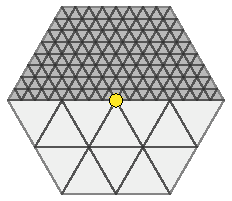
\includegraphics[height=3cm]{images/refine_interface/centre_input.pdf}};

\node (B) at (\xB, \yOne)
    {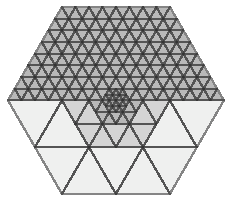
\includegraphics[height=3cm]{images/refine_interface/centre_refined.pdf}};

% ============================================================
%  DIVIDER (thin, no taller than the images: height 3cm -> +/-1.5cm)
% ============================================================
\draw[line width=0.1pt] (6.0cm, 1.5cm) -- (6.0cm, -1.5cm);

% ============================================================
%  NEIGHBOUR-NEIGHBOUR VERTEX GROUP
% ============================================================
\node (C) at (\xC, \yOne)
    {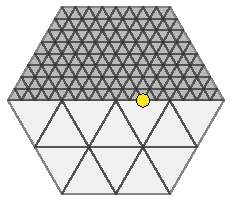
\includegraphics[height=3cm]{images/refine_interface/neighbour-neighbour_input.pdf}};

\node (D) at (\xD, \yOne)
    {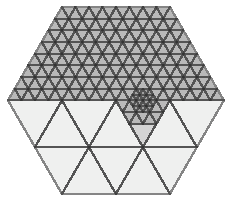
\includegraphics[height=3cm]{images/refine_interface/neighbour-neighbour_refined.pdf}};

\end{tikzpicture}%
}
\end{center}
\vspace{-3mm}
\caption{Two leaf meshes before and after applying the graded quadrisection operator from Definition~\robert{\ref{def:graded_vertex_quadrisection}} to a vertex (yellow) on the interface between level $0$ and level $2$. The target level is $3$, which results in one level of additional refinement around the vertices.}
\label{fig:refine_interface}
\end{figure}

\smallskip

Admissible domain sequences respect the geometric constraints necessary for linear independence and reproducing the correct cohomology. Unfortunately, in contrast to general domain sequences $\guidance{\alldomseqs}$, admissible domain sequences are not closed under the quadrisection operators $\quadriF(\domseq[\L], \cdot)$ \robert{and} $\quadriVup{\targetlevel}(\domseq[\L], \cdot)$, meaning that they are maps $\allpartitions \to \guidance{\alldomseqs}$. Thus, naive refinement of admissible domain sequences can reintroduce inadmissible geometry, for example a pinch vertex. This is exactly why Section~\ref{subsec:adaptive_loop} sets up a padding step that repairs these geometric defects and turns the domain sequence into a admissible domain sequence again.



\FloatBarrier

\section{Implementation and adaptive loop}
\label{subsec:adaptive_loop}

This section turns the constructions of Section~\ref{sec:construction_of_hierarchical_subdiv_spaces} into a working adaptive algorithm. Given an admissible domain sequence $\domseq$, the active DoFs $\activeDoFSet{k}{}(\domseq)$ follow from Definition~\ref{def:active_k_form_dofs} level by level --- Algorithm~\ref{alg:buildactivedofs} in Appendix~\ref{app:active_dof_pseudocode} evaluates it directly --- and the adaptive subdivision matrix $\Amat{k}{\activeDoFs}{\L}$ collects the corresponding columns of $\Amat{k}{\l}{\L}$ block by block as in Equation~\eqref{eq:hierarchical_matrix_blocks}. What remains is to embed this machinery in a standard \textsc{Solve}--\textsc{Estimate}--\textsc{Mark}--\textsc{Refine}--\textsc{Pad} adaptive loop, where the additional \textsc{Pad} restores the domain sequence output by \textsc{Refine} to an admissible one (Definition~\ref{def:subdiv_partition}) after each refinement via pinch resolution, confinement padding, and grading.

The loop used in the numerical experiments consists of the steps
\begin{equation}
\begin{tikzcd}
    \textsc{Solve} \arrow[r] & \textsc{Estimate} \arrow[r] & \textsc{Mark} \arrow[r] & \textsc{Refine} \arrow[r] & \textsc{Pad} \arrow[llll, rounded corners=0pt, to path={(\tikztostart.south) -- ([yshift=-1.em]\tikztostart.south) -- ([yshift=-1.em]\tikztotarget.south) -- (\tikztotarget.south)}]
\end{tikzcd}
\end{equation}

and is initialized with a admissible domain sequence $\domseq^0$. Throughout the adaptive loop, the general picture of the computational objects in Section~\ref{subsec:computational_representations} stays the same, the loop only refines $\domseq$ iteratively, and with that the active DoFs $\activeDoFSet{k}{}(\domseq)$ and the adaptive subdivision $k$-form spaces $\hierSDFspace{k}{\domseq}{\L}$. The \textsc{Pad} step is necessary because the \textsc{Refine} step only guarantees $\domseq^{\mathrm{refine}} \in \guidance{\alldomseqs}$, not $\domseq^{\mathrm{refine}} \in \allpartitions$, see Definition~\ref{def:subdiv_partition}. This means that the \textsc{Pad} step effectively restores linear independence and exactness of the complex.

\subsection{Solve}
\label{subsec:solve}

The details of the \textsc{Solve} step are typically problem-specific. The common thread for methods using subdivision differential forms is that the bilinear forms that constitute the weak formulation are first assembled using the spaces $\FEECspace{k}{\L}$ on $\T_\L$ and then unrefined to the spaces $\hierSDFspace{k}{\domseq}{\L}$ using the adaptive subdivision matrices $\Amat{k}{\activeDoFs}{\L}$ as in Equation~\eqref{eq:unrefinement}, see~\cite{Piel.2026}. The matrices of $\FEECspace{k}{\L}$ do not change during the adaptive loop because $\T_\L$ is fixed. A step changes only the selection of active DoFs, so its cost is the recomputation of the active DoFs $\activeDoFSet{k}{}$ followed by one sparse triple product per bilinear form. The unrefined matrices of the adaptive space inherit the density and the conditioning from the subdivision basis, which is where the cost of the method reappears. Section~\ref{subsubsec:cl_performance} measures both for an adaptive algorithm solving the mixed vector Laplace problem from Section~\ref{subsec:vector_laplace} and compares them to the reference run using $\FEECspace{k}{\L}$.

\subsection{Estimation}
\label{subsec:estimate}

We compute error indicators $\eta_{\l,\coarseIdxone}$ per leaf face $\face{\l}{\coarseIdxone} \in  \leafF{}(\domseq[\L])$ of the domain sequence $\domseq[\L]$. The residual is evaluated on the finest level $\L$ and then aggregated to the coarse parent faces:
\begin{equation}
    \label{eq:project_estimator_on_L_to_partition}
    \eta^2_{\l,\coarseIdxone} = \sum\limits_{\face{\L}{\fineIdxone} \; \in \; \Aop{}{\l}{\L}(\face{\l}{\coarseIdxone})} \eta^2_{\L,\fineIdxone},
\end{equation}
where $\eta^2_{\L,\fineIdxone}$ is evaluated in $\FEECspace{k}{\L}$. Any indicator that can be evaluated per face of $\T_\L$ drives the loop through Equation~\eqref{eq:project_estimator_on_L_to_partition}. The experiments of Section~\ref{subsec:vector_laplace} use the residual indicator of~\cite{Demlow.2014} for the mixed vector Laplace problem, stated for that test case in Equation~\eqref{eq:cl_estimator}.

Figure~\ref{fig:pipeline_marking_a} shows an example domain sequence with residual $\eta^2_{\l,\coarseIdxone}$. In the following, we will refer to $\eta^2$ and $\rho^2$ as the \emph{total} and \emph{refinable} residuals, respectively, defined as
\begin{equation}
    \label{def:total_and_refinable_residuals}
    \eta^2 = \sum\limits_{\l=\lzero}^{\L} \; \eta^2_\l \qquad \text{and} \qquad \rho^2 = \sum\limits_{\l=\lzero}^{\L-1} \; \eta^2_\l = \eta^2 - \eta^2_{\L} \qquad \text{with} \qquad \eta^2_{\l} = \sum\limits_{\face{\l}{\coarseIdxone} \; \in \; \F(\domseq_\l)} \eta^2_{\l,\coarseIdxone}.
\end{equation}
The refinable residual discards the contributions of faces $\face{\L}{\coarseIdxone}$ on level $\L$ of the admissible domain sequence $\domseq$. We measure this refinable residual because faces cannot be refined beyond level $\L$ without global mesh refinement to extend the mesh hierarchy. For this reason, the residual accumulated on level $\L$ can no longer be decreased. In fact, we find that
\begin{equation}
    \label{eq:saturation_rate}
    \rho^2 / \eta^2 = 1 - \eta^2_\L / \eta^2 \eqqcolon \xi
\end{equation}
This \emph{saturation rate} $\xi \in [0,1]$ provides a good analytic tool to understand the fraction of the overall estimator $\eta$ that cannot be decreased further through additional refinement.

% -----------------------------------------------------------------------
% CUT CANDIDATE (2026-08-21): this Example is superseded by the indicator
% relocated to Section~\ref{subsec:vector_laplace}, Equation (eq:cl_estimator).
% Kept here in \tobecut so both versions can be compared in the PDF; delete
% this banner together with the block once the relocated version is settled.
% -----------------------------------------------------------------------
%\tobecut{
%\begin{example}[Vector Laplace estimator]
%For the mixed vector Laplace problem with $(\sigma_h, u_h) \in \hierSDFspace{0}{\domseq}{\L} \times \hierSDFspace{1}{\domseq}{\L}$ from Section~\ref{subsec:vector_laplace}, the basis functions are piecewise linear approximations of the subdivision limit functions. Writing $\iota \colon \hierSDFspace{k}{\domseq}{\L} \hookrightarrow \FEECspace{k}{\L}$ for the inclusion of the hierarchical space into the fine FEEC space, $\extd (\iota u_h)$ is piecewise constant in $\FEECspace{2}{\L}$ and $\boldsymbol{\delta}\extd (\iota u_h)$ vanishes elementwise, while its contribution appears in the curl jumps across edges. In $\FEECspace{2}{\L}$, the indicator takes the form
%\begin{equation}
%\begin{aligned}
%    \eta_{\L,\fineIdxone}^2 = \quad &\checkit{\sum\limits_{\face{\L}{\coarseIdxone} \,\in\, \F_\L}} \!\! \robert{h_{\face{\L}{\fineIdxone}}^2} \big( \|f - \extd \sigma_h\|_{L^2(\face{\L}{\fineIdxone})}^2 + \checkit{\|\sigma_h + \boldsymbol{\delta} u_h\|_{L^2(\face{\L}{\fineIdxone})}^2} \big) \\
%    + &\checkit{\sum\limits_{\edge{\L}{\fineIdxtwo} \, \in \, \E_\L}} \robert{h_e} \big\|[\![\mathrm{curl}(u_h)]\!]\big\|_{L^2(\edge{\L}{\fineIdxtwo})}^2.
%\end{aligned}
%\end{equation}
%The first sum contains the elementwise residuals of both equations, and the second sum contains the %curl jump across interior edges $e$ of the fine mesh $\T_\L$. The per-face indicator $\eta_{\L,%\fineIdxone}^2$ on level $\L$ can be translated back to the admissible domain sequence $\domseq$ using %Equation~\eqref{eq:project_estimator_on_L_to_partition}.
%\end{example}
%} % end \tobecut of the superseded estimator example

\noindent We now have estimators $\eta_{\l,\coarseIdxone}$ per face of the admissible domain sequence $\domseq$. However, the atomic units of refinement in our scheme are vertex stars because they provide additional structure for the padding step, see Section~\ref{subsec:termination}. To enable vertex-based refinement for the adaptive algorithm, we need to sum up the face estimators $\eta_{\l,\coarseIdxone}$ to vertex estimators as shown in Figure~\ref{fig:pipeline_marking_b}. 

\newcommand{\markableVerts}{\bar{\V}}
For this operation, we use an area-weighted average of the faces in the leaf star of a vertex. Since the leaf star is independent of the vertex level, we assign a vertex-based residuals to the finest vertex on level $\L$. Thus, we consider the set of markable vertices
\begin{equation}
    \markableVerts(\domseq[\L]) \; \coloneq \; \bigcup\limits_{\l = \lzero}^{\L} \Aop{}{\l}{\L} \, \big( \V_\l (\domseq[\L]) \big) \;\; \subseteq \; \V_\L(\T_\L),
\end{equation}
where the notation $\markableVerts(\domseq[\L])$ indicates that all vertices in $\V(\domseq[\L])$ were flattened to level $\L$. The vertex residual $\nu_\coarseIdxtwo$ associated to a markable vertex $\vertex{\L}{\coarseIdxtwo} \in \markableVerts(\domseq[\L])$ is defined by
\begin{equation}
    \label{eq:vertex_residual}
    \nu^2_\coarseIdxtwo = \tfrac{1}{a_\coarseIdxtwo} \sum\limits_{\face{\l}{\coarseIdxone} \; \in \; \simplexsubset{2}{}} \eta^2_{\l,\coarseIdxone},
    \qquad \mathrm{where} \qquad
    a_\coarseIdxtwo = \sum\limits_{\face{\l}{\coarseIdxone} \; \in \; \simplexsubset{2}{}} \mathrm{area}(\face{\l}{\coarseIdxone})
\end{equation}
and $\simplexsubset{2}{} = \FVleaf{}(\vertex{\L}{\coarseIdxtwo}) \setminus \F_\L(\T_\L)$ contains all faces in the leaf star that are not on level $\L$ and can thus be refined to reduce the residual.Dividing by the cumulative area $a_\coarseIdxtwo$ of the faces rescales the integral face estimator to a density per vertex. This rescaling makes the marking roughly level- and valence-agnostic. Otherwise, the contribution of coarse faces would be weighted higher and their adjacent vertices would be over-represented during the Dörfler marking step.

\begin{figure}%[htbp]
    \centering
    \begin{subfigure}[b]{0.3\textwidth}
        \centering
        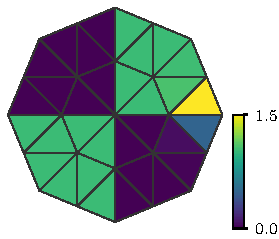
\includegraphics[width=\textwidth]{images/pipeline/pipeline_fig1a.pdf}
        \caption{Coarse domain sequence coloured by the per-face residual $\eta^2_{\l,\coarseIdxone}$ from Equation~\eqref{eq:project_estimator_on_L_to_partition}. }
        \label{fig:pipeline_marking_a}
    \end{subfigure}\hfill
    \begin{subfigure}[b]{0.3\textwidth}
        \centering
        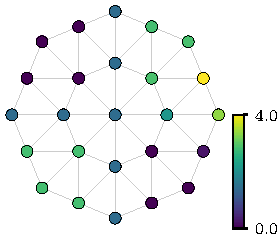
\includegraphics[width=\textwidth]{images/pipeline/pipeline_fig1b.pdf}
        \caption{Per-vertex error residual $\nu^2_\coarseIdxtwo$ after applying Equation~\eqref{eq:vertex_residual}}
        \label{fig:pipeline_marking_b}
    \end{subfigure}\hfill
\begin{subfigure}[b]{0.3\textwidth}
        \centering
        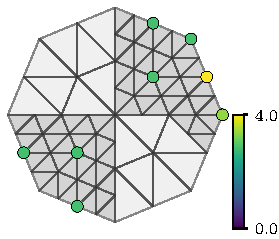
\includegraphics[width=\textwidth]{images/pipeline/pipeline_fig1c.pdf}
        \caption{Domain sequence after refining the leaf stars of marked vertices to their target levels.}
        \label{fig:pipeline_marking_c}
    \end{subfigure}
    \caption{Visualisations of the individual stages of the \textsc{Mark} and \textsc{Refine} steps.}
    \label{fig:pipeline_marking}
\end{figure}

\subsection{Marking}
\label{subsec:mark}

Our code marks vertices rather than faces. This enables us to use the graded vertex quadrisection operator $\quadriVup{\targetlevel}$ to refine single vertex stars. We rank the markable vertices $\markableVerts(\domseq[\L])$ by the vertex estimator $\nu_\coarseIdxtwo$, see Equation~\eqref{eq:vertex_residual}. For this purpose, we enumerate the markable vertices in order of decreasing residual, so that $\nu_{\coarseIdxtwo_1} \geq \nu_{\coarseIdxtwo_2} \geq \ldots \geq \nu_{\coarseIdxtwo_{\vert \markableVerts(\domseq[\L]) \vert}}$.

Dörfler marking~\citep{Doerfler.1996} marks the set $\markableVerts^\mathrm{mark} \coloneq \{ \vertex{\L}{\coarseIdxtwo_1}, \, \dots, \, \vertex{\L}{\coarseIdxtwo_q} \} \subseteq \markableVerts(\domseq[\L])$ by greedily selecting the first $q$ vertices with the largest estimators such that the \emph{marked refinable residual}
\begin{equation}
    \label{eq:marked_refinable_residual}
    \rho^2_{\R_\theta} \; \coloneqq \sum\limits_{\face{\l}{\coarseIdxone} \; \in \; \R_\theta} \eta^2_{\l, \coarseIdxone}, \qquad \text{where} \qquad \R_\theta = \bigcup\limits_{p=1}^q \FVleaf{} ( \vertex{\L}{\coarseIdxtwo_p} ) \setminus \F_\L(\T_\L),
\end{equation}
captures at least a fraction $\theta$ of the refinable residual $\rho$ of Equation~\eqref{def:total_and_refinable_residuals}, i.e.
\begin{equation}
    \label{eq:doerfler_selection}
    \rho_{\R_\theta} \; \geq \; \theta \, \rho
\end{equation}
where $\theta \in (0, 1]$ is the Dörfler parameter. The set $\R_\theta$ collects all the faces that are refined during the \textsc{Refine} step, see Section~\ref{subsec:refine}. Faces on level $\L$ are excluded again, so $\rho_{\R_\theta}$ is a restriction of the refinable residual $\rho$ rather than of the total residual $\eta$.

\subsection{Refinement}
\label{subsec:refine}

The \textsc{Refine} step refines the marked faces $\face{\l}{\coarseIdxone} \in \R_\theta$ in the leaf stars of the selected vertices $\vertex{\L}{\coarseIdxtwo} \in \markableVerts^\mathrm{mark}$ from Equation~\eqref{eq:marked_refinable_residual} as shown in Figure~\ref{fig:pipeline_marking_c}. We denote by $\lmax{}_{,\coarseIdxtwo} = \lmax \big( \FVleaf{}(\vertex{\L}{\coarseIdxtwo}) \big)$ and similarly $\lmin{}_{,\coarseIdxtwo} = \lmin \big( \FVleaf{}(\vertex{\L}{\coarseIdxtwo}) \big)$ the finest level and coarsest levels of faces occurring in the leaf star of $\vertex{\L}{\coarseIdxtwo}$ according to Definition~\ref{def:level_range}. 

The \textsc{Refine} step homogenises the leaf star of each marked vertex $\vertex{\L}{\coarseIdxtwo}$ at one level beyond the finest level it currently carries unless is already carries the finest level $\L$. Thus, the target level of the graded vertex quadrisection operator $\quadriVup{\targetlevel_\coarseIdxtwo}(\domseq[\L], \vertex{\L}{\coarseIdxtwo})$ of Definition~\ref{def:graded_vertex_quadrisection} is given by $\targetlevel_\coarseIdxtwo = \min(\lmax{}_{,\coarseIdxtwo} \! + \! 1, \, \L)$. The target levels $\targetlevel_\coarseIdxtwo$ for all marked vertices must be computed on the fixed input domain sequence $\domseq[\L]$ before any refinement takes place to avoid a cascade of ever increasing target levels. 

\smallskip

\noindent The result of the \textsc{Refine} step is the domain sequence $\domseq[\L]^{\mathrm{refine}}$ given by
\begin{enumerate}[topsep=3pt, itemsep=-2pt]
    \item initialise $\domseq[\L]^0 = \domseq[\L]$,
    \item refine vertex stars iteratively for all $\vertex{\L}{\coarseIdxtwo_p} \in \markableVerts^\mathrm{mark}$ with $p = 1, \, \dots, \, \vert \markableVerts^\mathrm{mark}\vert$ to obtain
    \begin{equation}
        \domseq[\L]^{p} = \quadriVup{\targetlevel_{\coarseIdxtwo_p}} \big( \domseq[\L]^{p-1}, \, \vertex{\L}{\coarseIdxtwo_p} \big),
    \end{equation}
    \vspace{-7mm}
    \item set $\domseq[\L]^{\mathrm{refine}} \coloneq \domseq[\L]^{\vert \markableVerts^\mathrm{mark} \vert}$.
\end{enumerate}
Because the expected target levels $\targetlevel_{\coarseIdxtwo}$ are computed on the fixed input domain sequence $\domseq$ and each quadrisection only ever homogenises a star upward to $\targetlevel_{\coarseIdxtwo}$, the order in which the $\vertex{\L}{\coarseIdxtwo} \in \markableVerts^\mathrm{mark}$ are processed does not affect the resulting partition $\domseq[\L]^{\mathrm{refine}}$.
\FloatBarrier

\subsection{Padding}
\label{subsec:padding}

The \textsc{Refine} step in the previous section produces the domain sequence $\domseq[\L]^{\mathrm{refine}}$. Crucially, $\domseq[\L]^{\mathrm{refine}}$ is not a admissible domain sequence because $\domseq[\L]^{\mathrm{refine}}$ might now contain confined faces, pinch vertices, or boundary pinch vertices. The \textsc{Pad} step described in this section repairs these defects and turns $\domseq[\L]^{\mathrm{refine}}$ into an admissible domain sequence $\domseq[\L]^{\mathrm{pad}}$. The goal is to keep the padded faces added during this process to a minimum to avoid inflating the number of DoFs in non-marked regions. The only exception is some optional grading that we apply around vertices whose leaf star covers too many levels.

The \textsc{Pad} step needs no machinery beyond the quadrisection operators $\quadriF$ \robert{and} $\quadriVup{\targetlevel}$ of Section~\ref{subsec:refinement_operators}, since every padding substep is a quadrisection of either a vertex star or a set of confined faces.

\robert{Each of the three substeps has the same shape. A \emph{candidate set} of vertices or of leaf faces is tested against the substep's predicate on the unmutated domain sequence, every candidate that fires is repaired, and the candidates of the next round are read off the faces that the repair has actually refined. Testing the whole candidate set before repairing any of it makes a round independent of the order in which its repairs are applied. What makes the restricted candidate set of the next round sufficient is that a quadrisection can change a predicate only at the vertices of the faces it refines, and only on the level of those faces.}

% SUPERSEDED (2026-08-23): stated for a single-level face set, and its proof
% claims $\quadriF$ "changes the region $\M_{\l+1}$ and no other", which is false
% for the multi-level operator of Definition~\ref{def:face_quadrisection_operator}.
% Replaced by the version below, which runs over all levels at once and therefore
% also covers $\quadriVup{\targetlevel}$ in one application rather than factor by
% factor. Kept for cherry-picking.
\tobecut{
\begin{lemma}[Locality of the padding predicates, single level]
    Let $\domseq[\L] \in \alldomseqs$, let $\simplexsubset{2}{\l} \subseteq \leafF{\l}(\domseq[\L])$ be a set of leaf faces on level $\l$, and let $\domseq[\L]' \coloneq \quadriF(\domseq[\L], \simplexsubset{2}{\l})$ with refinement fans $\refFan{\lone}'$. Then
    \begin{equation}
        \refFan{\lone}' \big( \vertex{\lone}{\coarseIdxtwo} \big) \; = \; \refFan{\lone} \big( \vertex{\lone}{\coarseIdxtwo} \big)
    \end{equation}
    holds for every level $\lone \neq \l$ and every vertex $\vertex{\lone}{\coarseIdxtwo} \in \V_\lone(\T_\lone)$, and on level $\lone = \l$ for every vertex that is not a vertex of a face of $\simplexsubset{2}{\l}$. Consequently,
    \begin{enumerate}[topsep=3pt, itemsep=-2pt]
        \item a vertex that is neither a pinch nor a boundary pinch of $\domseq[\L]$ on level $\lone$ is neither one of $\domseq[\L]'$ on level $\lone$, unless $\lone = \l$ and it is a vertex of a face of $\simplexsubset{2}{\l}$, and
        \item a leaf face of $\domseq[\L]$ that is unconfined in $\domseq[\L]$ and is still a leaf face of $\domseq[\L]'$ is unconfined in $\domseq[\L]'$, unless it lies on level $\l$ and shares a vertex with a face of $\simplexsubset{2}{\l}$.
    \end{enumerate}
\end{lemma}
} % end \tobecut of the single-level locality lemma

\begin{lemma}[\robert{Locality of the padding predicates}]
    \label{lemma:pad_locality}
    \robert{Let $\domseq[\L] \in \alldomseqs$, let $\simplexsubset{2}{}$ be a set of leaf faces of $\domseq[\L]$ below level $\L$, that is $\simplexsubset{2}{\l} \subseteq \leafF{\l}(\domseq[\L])$ for every $\l < \L$, and let $\domseq[\L]' \coloneq \quadriF(\domseq[\L], \simplexsubset{2}{})$ with refinement fans $\refFan{\lone}'$. Then
    \begin{equation}
        \label{eq:pad_locality}
        \refFan{\lone}' \big( \vertex{\lone}{\coarseIdxtwo} \big) \; = \; \refFan{\lone} \big( \vertex{\lone}{\coarseIdxtwo} \big)
    \end{equation}
    holds on every level $\lone$ for every vertex $\vertex{\lone}{\coarseIdxtwo} \in \V_\lone(\T_\lone)$ that is not a vertex of a face of the slice $\simplexsubset{2}{\lone}$. Consequently,
    \begin{enumerate}[topsep=3pt, itemsep=-2pt]
        \item a vertex that is neither a pinch nor a boundary pinch of $\domseq[\L]$ on level $\lone$ is neither one of $\domseq[\L]'$ on level $\lone$, unless it is a vertex of a face of $\simplexsubset{2}{\lone}$, and
        \item a leaf face of $\domseq[\L]$ on level $\lone$ that is unconfined in $\domseq[\L]$ and is still a leaf face of $\domseq[\L]'$ is unconfined in $\domseq[\L]'$, unless it shares a vertex with a face of $\simplexsubset{2}{\lone}$.
    \end{enumerate}
    The predicates of a vertex or a face therefore change only on the level of the faces that were refined beneath it, and only in the one-ring of those faces read on that level.}
\end{lemma}
\begin{proof}
    \robert{By Definition~\ref{def:face_quadrisection_operator}, $\quadriF(\domseq[\L], \simplexsubset{2}{})$ enlarges the region $\M_{\lone+1}$ by $\Aop{}{\lone}{\lone+1}(\simplexsubset{2}{\lone})$ on every level, so it enlarges the ancestor patch $\ancestorPatch{\M_{\lone+1}}$ by exactly the slice $\simplexsubset{2}{\lone}$ and by nothing else. The refinement fan $\refFan{\lone}(\vertex{\lone}{\coarseIdxtwo}) = \FVl{\lone}(\vertex{\lone}{\coarseIdxtwo}) \cap \ancestorPatch{\M_{\lone+1}}$ of Definition~\ref{def:refinement_fan} can therefore only change at a vertex whose mesh star on level $\lone$ meets $\simplexsubset{2}{\lone}$, that is at a vertex of a face of $\simplexsubset{2}{\lone}$, which is~\eqref{eq:pad_locality}. Note that the levels do not interact: the slice $\simplexsubset{2}{\lone}$ alone decides what changes on level $\lone$, whatever the other slices contain. Both consequences follow because the three predicates are read off the refinement fan alone: the pinch of Definition~\ref{def:pinch_vertex} and the boundary pinch of Definition~\ref{def:boundary_pinch} count its arcs, and the confined face of Definition~\ref{def:confined_face} asks whether one of its vertices has an empty fan.}
\end{proof}

\robert{Two remarks on the reach of the lemma. First, it says nothing about the faces that $\quadriF$ creates: the children of $\simplexsubset{2}{\lone}$ are new leaf faces on level $\lone\!+\!1$ and have to be tested, which is what the candidate sets below do. It does settle the new \emph{vertices}, which are born on level $\lone\!+\!1$ with an empty refinement fan and are therefore neither pinches nor boundary pinches there. Second, the lemma covers the graded vertex quadrisection in a single application and not factor by factor. Its proof uses only that the ancestor patch on level $\lone$ grows by the slice $\simplexsubset{2}{\lone}$ and by nothing else, and Definition~\ref{def:graded_vertex_quadrisection} grows it by
\begin{equation}
    \label{eq:graded_quadrisection_patch_growth}
    \ancestorPatch{\tilde{\M}_{\lone+1}} \; \setminus \; \ancestorPatch{\M_{\lone+1}} \; \subseteq \bigcup\limits_{\substack{w \, \in \, W \\ \lone \, < \, \targetlevel(w)}} \FVanc{\lone}(w),
\end{equation}
as computed after that definition. So the same argument applies with the slice read as the right-hand side of~\eqref{eq:graded_quadrisection_patch_growth}: the vertices whose predicates can have changed under $\quadriVup{\targetlevel}(\cdot, W)$ are the vertices of the star ancestries of $W$, each read on the level of the face that carried it.}

\guidance{Why~\eqref{eq:graded_quadrisection_patch_growth} rather than an appeal to $\quadriVup{\targetlevel}$ being an instance of $\quadriF$: it is one, as far as the two formulas go, but not one that satisfies this lemma's hypothesis. The lemma asks for $\simplexsubset{2}{} \subseteq \leafMesh(\domseq[\L])$, whereas a face of $\FVanc{\lone}(w)$ need not lie in $\M_\lone$ at all on the input --- it can still be covered by a coarser leaf face, and only the coarser slices of the same application put it into the region. The growth of the ancestor patch is what the proof actually uses, and it is available for both operators.}


\paragraph{Resolving vertex pinches.}

We scan every level of the refined domain sequence $\domseq[\L]^\mathrm{refine}$ and every vertex of that level to build the set of pinches
\begin{equation}
    \V^{\mathrm{pinch}}(\domseq[\L]^{\mathrm{refine}}) \coloneq \big\{ \vertex{\l}{\coarseIdxtwo} \in \V(\domseq[\L]^{\mathrm{refine}}) \; \colon \; \vertex{\l}{\coarseIdxtwo} \text{ is a (boundary) pinch of } \domseq[\L]^{\mathrm{refine}} \text{ at level } \l \big\}
\end{equation}
according to Definitions~\ref{def:pinch_vertex} and~\ref{def:boundary_pinch}. Note that the pinch test is applied at every level at which the vertex exists in the domain sequence, not only at its finest one. The domain sequence $\domseq[\L]^{\mathrm{pinch}} \coloneq \domseq[\L]^{\vert \V^{\mathrm{pinch}} \vert}$ with all pinches resolved is obtained from the iteration
\begin{equation}
    \label{eq:pinch_resolved_subdiv_partition}
    \domseq[\L]^p = \quadriVup{\l + 1} \big( \domseq[\L]^{p-1}, \, (\vertex{\l}{\coarseIdxtwo})_p \big) \qquad \text{for all} \qquad (\vertex{\l}{\coarseIdxtwo})_p \in \V^{\mathrm{pinch}}(\domseq[\L]^{\mathrm{refine}}),
\end{equation}
where $p \in \{1, \, \dots, \, \vert \V^{\mathrm{pinch}}(\domseq[\L]^{\mathrm{refine}}) \vert \}$ is an enumeration of the pinch vertices and $\domseq[\L]^0 = \domseq[\L]^\mathrm{refine}$ is initialised to the domain sequence after the \textsc{Refine} step.

\guidance{To be reworded once the iteration below is settled: $\domseq[\L]^{\mathrm{pinch}}$ is the fixed point of that iteration and not the last element $\domseq[\L]^{\vert \V^{\mathrm{pinch}} \vert}$ of a single enumeration. Equations~\eqref{eq:pinch_resolved_subdiv_partition} should keep the enumeration but produce $\domseq[\L]^{\mathrm{pinch},k}$ of round $k$, and the definition of $\domseq[\L]^{\mathrm{pinch}}$ should move to step~4 of the iteration. That also gives the index set $\V^{\mathrm{pinch}}$ a definition per round, which it currently lacks in the iteration counts.}

The target level $\targetlevel = \l\!+\!1$ is what merges the arcs. The refinement arcs at level $\l$ are separated by faces that are not refined beyond $\l_p$. Grading the leaf star to $\l\!+\!1$ refines every one of them, so the fan at level $\l$ becomes the whole mesh star. A single flat quadrisection does not suffice, because the separation between the refinement arcs can be covered by a leaf face at a level well below $\l$, in which case one round lifts it only by one level and leaves the arcs separated.

Detection and repair are separate phases. The whole set $\V^{\mathrm{pinch}}(\domseq[\L]^{\mathrm{refine}})$ of pinch vertices is collected before any of its elements is repaired, so resolving one vertex cannot hide a pinch at another, and the iteration above is well defined.

\guidance{This paragraph now describes one round of the iteration below rather than the whole substep. Consider inserting ``within one round'' so that it does not read as a claim about $\domseq[\L]^{\mathrm{pinch}}$.}

\robert{What Equations~\eqref{eq:pinch_resolved_subdiv_partition} do not certify is that no pinch is left. By Lemma~\ref{lemma:pad_locality} a repair changes the refinement fans at the vertices of the faces it refines, and a vertex that was not a pinch before can be one afterwards. The substep is therefore run as an iteration over a candidate set:
\begin{enumerate}[topsep=3pt, itemsep=-2pt]
    \item initialise $\domseq[\L]^{\mathrm{pinch},0} \coloneq \domseq[\L]^{\mathrm{refine}}$ and the candidate set $\V^{\mathrm{cand},0} \coloneq \V(\domseq[\L]^{\mathrm{refine}})$ to all vertices of the domain sequence on all levels, see Equation~\eqref{eq:vertices_of_domseq},
    \item in round $k \geq 1$, detect the pinches among the candidates on the unmutated $\domseq[\L]^{\mathrm{pinch},k-1}$,
    \begin{equation}
        \label{eq:pinch_round_detection}
        \V^{\mathrm{pinch},k} \coloneq \big\{ \vertex{\l}{\coarseIdxtwo} \in \V^{\mathrm{cand},k-1} \; \colon \; \vertex{\l}{\coarseIdxtwo} \text{ is a (boundary) pinch of } \domseq[\L]^{\mathrm{pinch},k-1} \text{ at level } \l \big\},
    \end{equation}
    \vspace{-7mm}
    \item repair them by the iteration~\eqref{eq:pinch_resolved_subdiv_partition} to obtain $\domseq[\L]^{\mathrm{pinch},k}$, and collect the candidates of the next round from the faces that round $k$ has refined,
    \begin{equation}
        \label{eq:pinch_candidates}
        \V^{\mathrm{cand},k} \coloneq \big\{ \vertex{\lone}{\fineIdxone} \; \colon \; \vertex{\lone}{\fineIdxone} \text{ is a vertex of a face on level } \lone \text{ refined in round } k \big\},
    \end{equation}
    \vspace{-7mm}
    \item stop at the first round with $\V^{\mathrm{pinch},k} = \varnothing$ and set $\domseq[\L]^{\mathrm{pinch}} \coloneq \domseq[\L]^{\mathrm{pinch},k}$.
\end{enumerate}}

\robert{The candidate set~\eqref{eq:pinch_candidates} is exactly what Lemma~\ref{lemma:pad_locality} permits, and it differs from the one-ring of the repaired vertices in both directions. It is narrower, because a vertex enters as a candidate only on the level of the face that carried it and not on every level at which it exists. It is wider, because $\quadriVup{\l+1}$ refines faces on all levels between $\lmin$ and $\l$, and a face on a level $\lone < \l$ of the leaf star of $\vertex{\l}{\coarseIdxtwo}$ need not carry $\vertex{\l}{\coarseIdxtwo}$ as a vertex at all: a vertex born on level $\l$ can lie in the interior of an edge of the leaf face covering it, and then the candidates are its level-$\lone$ neighbours, which lie further out than its level-$\l$ ring.}

\robert{The repaired vertices themselves need not be carried over, which is the content of the next lemma. Its second half also bounds how often the iteration can repeat.}

\begin{lemma}[\robert{Pinch resolution spends its vertex}]
    \label{lemma:pinch_spent}
    \robert{Let $\vertex{\l}{\coarseIdxtwo}$ be a pinch of $\domseq[\L]$ on level $\l$ and let $\domseq[\L]' \coloneq \quadriVup{\l+1}(\domseq[\L], \vertex{\l}{\coarseIdxtwo})$. Then the refinement fan of $\vertex{\l}{\coarseIdxtwo}$ in $\domseq[\L]'$ is its entire mesh star,
    \begin{equation}
        \label{eq:pinch_spent}
        \refFan{\lone}' \big( \vertex{\lone}{\coarseIdxtwo} \big) \; = \; \FVl{\lone} \big( \vertex{\lone}{\coarseIdxtwo} \big),
    \end{equation}
    on every level $\lone \leq \l$ at which $\vertex{\l}{\coarseIdxtwo}$ exists, and the same holds in every domain sequence obtained from $\domseq[\L]'$ by further quadrisection. In particular, $\vertex{\l}{\coarseIdxtwo}$ is never again a pinch or a boundary pinch on a level $\lone \leq \l$.

    Consequently, the number $q^{\mathrm{pinch}}$ of productive rounds of the pinch iteration is bounded by the number of vertex-level pairs the domain sequence carries,
    \begin{equation}
        \label{eq:pinch_rounds}
        q^{\mathrm{pinch}} \; \leq \; \sum\limits_{\l = \lzero}^{\L-1} \big\vert \V_\l(\M_\l) \big\vert,
    \end{equation}
    and the iteration performs $q^{\mathrm{pinch}} \! + \! 1$ rounds in total.}
\end{lemma}
\begin{proof}
% SUPERSEDED (2026-08-23): read off the iterative algorithm, which is no longer
% the definition of the operator. Replaced by the two-line argument below, which
% reads the closed form of Definition~\ref{def:graded_vertex_quadrisection}
% directly. Kept for cherry-picking.
    \tobecut{By the iterative algorithm of Remark~\ref{rem:graded_quadrisection_algorithm} the operator refines the coarsest slice of the leaf star of $\vertex{\l}{\coarseIdxtwo}$ once per level, and each such refinement raises the coarsest level of that leaf star by one, so the leaf star of $\vertex{\l}{\coarseIdxtwo}$ in $\domseq[\L]'$ carries no face below level $\l\!+\!1$. Let $\lone \leq \l$ and let $\face{\lone}{\coarseIdxone} \in \FVl{\lone}(\vertex{\lone}{\coarseIdxtwo})$. The faces of the mesh star $\FVl{\L}(\vertex{\L}{\coarseIdxtwo})$ that descend from $\face{\lone}{\coarseIdxone}$ are covered by leaf faces on levels $\geq \l\!+\!1 > \lone$, so $\face{\lone}{\coarseIdxone} \in \ancestorPatch{\M_{\lone+1}}$ and hence $\face{\lone}{\coarseIdxone} \in \refFan{\lone}'(\vertex{\lone}{\coarseIdxtwo})$, which is~\eqref{eq:pinch_spent}.}

    \robert{Let $\lone \leq \l$ be a level at which $\vertex{\l}{\coarseIdxtwo}$ exists. By Definition~\ref{def:graded_vertex_quadrisection} with $\targetlevel = \l \! + \! 1$, the regions of $\domseq[\L]'$ contain $\Aop{}{\lone}{\lone+1}(\FVanc{\lone}(\vertex{\l}{\coarseIdxtwo}))$ on level $\lone \! + \! 1$, so every face of $\FVanc{\lone}(\vertex{\l}{\coarseIdxtwo})$ lies in $\ancestorPatch{\M'_{\lone+1}}$ and is refined beyond level $\lone$. That star ancestry is the mesh star $\FVl{\lone}(\vertex{\lone}{\coarseIdxtwo})$ by~\eqref{eq:star_ancestry_is_star}, so the refinement fan $\refFan{\lone}'(\vertex{\lone}{\coarseIdxtwo}) = \FVl{\lone}(\vertex{\lone}{\coarseIdxtwo}) \cap \ancestorPatch{\M'_{\lone+1}}$ of Definition~\ref{def:refinement_fan} is the whole mesh star, which is~\eqref{eq:pinch_spent}. The regions of a domain sequence only grow under the quadrisection operators, so~\eqref{eq:pinch_spent} survives every later refinement. A full refinement fan is a single arc and contains both extremes of a linear fan, so it is neither a pinch by Definition~\ref{def:pinch_vertex} nor a boundary pinch by Definition~\ref{def:boundary_pinch}. For the bound, every productive round repairs at least one pair of a vertex and a level, no pair is ever repaired twice by the first half, and pinches are detected only on levels $\l < \L$. The last round detects nothing and stops the iteration.}
\end{proof}

\robert{A round that detects nothing certifies more than its own emptiness. Every vertex whose refinement fan has changed since the previous detection is a candidate by Lemma~\ref{lemma:pad_locality}, so an empty round proves that no vertex of $\domseq[\L]^{\mathrm{pinch}}$ is a pinch or a boundary pinch on any level. The substep therefore has an exact postcondition: $\domseq[\L]^{\mathrm{pinch}}$ satisfies clauses~(ii) and~(iii) of Definition~\ref{def:subdiv_partition}.}

\guidance{Measured, for the discussion of the bound: the pinch iteration has never needed more than one productive round, neither at any step of the adaptive runs of Section~\ref{subsec:vector_laplace} nor in any of the exhaustive marking sweeps, so in practice it costs one repair round and one certifying round. The bound~\eqref{eq:pinch_rounds} is crude and depends on the mesh. Unlike the confinement iteration below, there is no bound by the number of levels here, because a repair on level $\l$ can open a pinch on any level $\leq \l$; that is the same mechanism that drives the outer loop, cf.\ Remark~\ref{rem:padding_chain}.}

\paragraph{Resolving confined faces.}

Similarly to resolving pinches, we iterate over all leaf faces $\face{\l}{\coarseIdxone}$ of the domain sequence $\domseq^{\mathrm{pinch}}$ to build the set of confined faces
\begin{equation}
    \F^{\mathrm{confined}} = \big\{ \face{\l}{\coarseIdxone} \in \leafF{\l}(\domseq[\L]^{\mathrm{pinch}}) \; \colon \; \face{\l}{\coarseIdxone} \text{\; is confined} \big\}
\end{equation}
according to Definition~\ref{def:confined_face}. The repaired domain sequence $\domseq[\L]^{\mathrm{confined}}$ is given by
\begin{equation}
    \label{eq:confined_faces_resolved_subdiv_partition}
    \domseq[\L]^{\mathrm{unconfined}} = \quadriF \big( \domseq[\L]^{\mathrm{pinch}}, \, \F^{\mathrm{confined}} \big).
\end{equation}
\guidance{Name clash to settle: this sentence and Equations~\eqref{eq:grading_subdiv_partition} call the result $\domseq[\L]^{\mathrm{confined}}$, while Equation~\eqref{eq:confined_faces_resolved_subdiv_partition} and the grading paragraph call it $\domseq[\L]^{\mathrm{unconfined}}$. The text from here on uses $\domseq[\L]^{\mathrm{unconfined}}$, since it names the property the substep establishes; the parallel with $\domseq[\L]^{\mathrm{pinch}}$, which names the defect just handled, would argue for $\domseq[\L]^{\mathrm{confined}}$ instead.}

% SUPERSEDED (2026-08-22): false whenever the neighbourhood of the confined face
% is refined two or more levels beyond \l, which g = 2 permits and which the L = 3
% run hits. Replaced by the iteration and by lemma:confined_children /
% cor:confinement_rounds below. Kept for cherry-picking.
\tobecut{In words, we refine every confined face by one level, because its children carry a vertex that is refinement-exterior at level $\l\!+\!1$ and are therefore unconfined.}

\robert{In words, we refine every confined face by one level. That does not in general leave a domain sequence without confined faces, because the children of a confined face on level $\l$ inherit its neighbourhood: if that neighbourhood is refined two or more levels beyond $\l$, then the child at the corner shared by the finer faces has no refinement-exterior vertex on level $\l\!+\!1$ either and is confined in turn. The substep is therefore iterated in the same shape as the pinch resolution:
\begin{enumerate}[topsep=3pt, itemsep=-2pt]
    \item initialise $\domseq[\L]^{\mathrm{unconfined},0} \coloneq \domseq[\L]^{\mathrm{pinch}}$ and the candidate set $\F^{\mathrm{cand},0} \coloneq \leafMesh(\domseq[\L]^{\mathrm{pinch}})$ to all leaf faces on all levels,
    \item in round $k \geq 1$, detect the confined faces among the candidates on the unmutated $\domseq[\L]^{\mathrm{unconfined},k-1}$,
    \begin{equation}
        \label{eq:confined_round_detection}
        \F^{\mathrm{confined},k} \coloneq \big\{ \face{\l}{\coarseIdxone} \in \F^{\mathrm{cand},k-1} \; \colon \; \face{\l}{\coarseIdxone} \text{ is confined in } \domseq[\L]^{\mathrm{unconfined},k-1} \big\},
    \end{equation}
    \vspace{-7mm}
    \item refine them level by level as in~\eqref{eq:confined_faces_resolved_subdiv_partition} to obtain $\domseq[\L]^{\mathrm{unconfined},k}$, and take the children of the faces just refined as the candidates of the next round,
    \begin{equation}
        \label{eq:confined_candidates}
        \F^{\mathrm{cand},k} \coloneq \Aop{}{\l}{\l+1} \big( \F^{\mathrm{confined},k} \big),
    \end{equation}
    \vspace{-7mm}
    \item stop at the first round with $\F^{\mathrm{confined},k} = \varnothing$ and set $\domseq[\L]^{\mathrm{unconfined}} \coloneq \domseq[\L]^{\mathrm{unconfined},k}$.
\end{enumerate}}

\robert{Here the children are not merely a sufficient candidate set but the only one needed, and that is what bounds the number of rounds.}

\begin{lemma}[\robert{Confinement padding confines only its own children}]
    \label{lemma:confined_children}
    \robert{Let $\domseq[\L] \in \alldomseqs$, let $\F^{\mathrm{confined}} \subseteq \leafMesh(\domseq[\L])$ be a set of leaf faces, every one of which is confined in $\domseq[\L]$, and let $\domseq[\L]'$ be the result of refining them level by level as in~\eqref{eq:confined_faces_resolved_subdiv_partition}. Then every leaf face of $\domseq[\L]'$ that is confined in $\domseq[\L]'$ and was not confined in $\domseq[\L]$ is a child of a face of $\F^{\mathrm{confined}}$.}
\end{lemma}
\begin{proof}
    \robert{The regions of a domain sequence only grow under quadrisection, so a refinement-exterior vertex can only lose that property and a confined face stays confined. The hypothesis therefore still holds at every level of the sweep, and it suffices to consider the refinement of the faces of $\F^{\mathrm{confined}}$ on one level $\l$.

    Let $\face{\lone}{\fineIdxone}$ be a leaf face of $\domseq[\L]$ that is unconfined, and let $\vertex{\lone}{\coarseIdxtwo}$ be one of its vertices that is refinement-exterior on level $\lone$. If $\lone \neq \l$, then $\refFan{\lone}(\vertex{\lone}{\coarseIdxtwo})$ is unchanged by Lemma~\ref{lemma:pad_locality}. If $\lone = \l$, then $\vertex{\l}{\coarseIdxtwo}$ is a vertex of no face of $\F^{\mathrm{confined}}$ on level $\l$: such a face is confined and therefore has no refinement-exterior vertex on level $\l$ by Definition~\ref{def:confined_face}, whereas $\vertex{\l}{\coarseIdxtwo}$ has an empty fan there. So $\refFan{\l}(\vertex{\l}{\coarseIdxtwo})$ is unchanged by Lemma~\ref{lemma:pad_locality} as well. In both cases $\vertex{\lone}{\coarseIdxtwo}$ stays refinement-exterior and $\face{\lone}{\fineIdxone}$ stays unconfined. The only faces of $\domseq[\L]'$ that are not faces of $\domseq[\L]$ are the children of $\F^{\mathrm{confined}}$.}
\end{proof}

\begin{corollary}[\robert{The confinement iteration advances one level per round}]
    \label{cor:confinement_rounds}
    \robert{Let $\l_k$ denote the coarsest level carrying a face of $\F^{\mathrm{confined},k}$. Then $\l_{k+1} \geq \l_k \! + \! 1$, and the number $q^{\mathrm{confined}}$ of productive rounds of the confinement iteration satisfies
    \begin{equation}
        \label{eq:confinement_rounds}
        q^{\mathrm{confined}} \; \leq \; \L - \l_1 \; \leq \; \L - \lzero.
    \end{equation}
    The iteration performs $q^{\mathrm{confined}} \! + \! 1$ rounds and returns a domain sequence $\domseq[\L]^{\mathrm{unconfined}}$ without confined leaf faces, that is, one satisfying clause~(i) of Definition~\ref{def:subdiv_partition}.}
\end{corollary}
\begin{proof}
    \robert{By Lemma~\ref{lemma:confined_children} the set $\F^{\mathrm{confined},k+1}$ is contained in the candidate set $\F^{\mathrm{cand},k}$ of~\eqref{eq:confined_candidates}, whose faces are children of faces of $\F^{\mathrm{confined},k}$ and hence lie on levels $\geq \l_k \! + \! 1$. No leaf face on level $\L$ is ever confined, because no face is refined beyond $\L$, so $\refFan{\L}$ is empty at every vertex and every vertex is refinement-exterior on level $\L$. Hence $\l_k \leq \L \! - \! 1$ for every productive round, which gives~\eqref{eq:confinement_rounds}. An empty round certifies that no leaf face is confined, since by Lemma~\ref{lemma:confined_children} every face whose confinement has changed since the previous detection is a candidate.}
\end{proof}

\robert{The cost of the iteration is therefore bounded by the number of levels rather than by the size of the mesh, and after the first round each round only tests the children of the faces the previous one refined. The number of productive rounds is the depth by which the neighbourhood of the deepest confined face is refined beyond it, so it is one exactly when no confined face is buried by more than one level, which is the case at all but one step of the adaptive runs of Section~\ref{subsec:vector_laplace}.}

\guidance{Measured, for the discussion of the bound: a confined face whose neighbourhood is refined $d$ levels beyond it costs exactly $d$ rounds, verified for $d = 1, \dots, 4$, and the output is a staircase in which each round refines only the corner child at the buried vertex. In the adaptive runs the deepest occurrence is $d = 2$, at one step of the $\L = 3$ run, and $d = 1$ everywhere else. Worth settling before it is claimed: the input to $\textsc{Pad}$ is a graded domain sequence of span at most $g$ refined by $\textsc{Refine}$, which would give $d \leq g\!+\!1$ and hence the constant bound $q^{\mathrm{confined}} \leq g\!+\!1 = 3$ rather than~\eqref{eq:confinement_rounds}. It is not immediate, because the grading step bounds the span of its own output and not of the input that the next $\textsc{Pad}$ receives, and on a hand-built input of depth $4$ with $g = 2$ the round count went up rather than down.}

\guidance{Note that $q$ now carries two more meanings, $q^{\mathrm{pinch}}$ of Lemma~\ref{lemma:pinch_spent} and $q^{\mathrm{confined}}$ above, on top of the form degree, the marked-vertex count and the pass count of Section~\ref{subsec:termination}. If the overloading is resolved, these two should move with it.}

\paragraph{Grading leaf stars.}

The grading is supposed to smooth out transitions across vertices $\vertex{\l}{\coarseIdxtwo}$ of $\domseq^{\mathrm{unconfined}}$ whose leaf stars still have large level spans, see Definition~\ref{def:level_range}. Unlike the pinch resolution and the confinement padding, the grading step does not restore exactness or linear independence but is intended to improve the conditioning of the matrix-vector system and to avoid numerical artifacts in the transition areas. Thus, grading is an optional padding step.

The predicate to identify the vertices $(\vertex{\l}{\coarseIdxtwo})$ to grade is the level span $\mu_\coarseIdxtwo \coloneq \lmax{}_{,\coarseIdxtwo} - \lmin{}_{,\coarseIdxtwo}$ of its leaf star $\FVleaf{}(\vertex{\l}{\coarseIdxtwo})$. The detection algorithm fixes a maximum level span $g \in \mathbb{N}$ and assembles the set
\begin{equation}
    \V^{\mathrm{grading}}(\domseq[\L]^\mathrm{confined}) \coloneq \big\{ \vertex{\l}{\coarseIdxtwo} \in \V(\domseq[\L]^\mathrm{confined}) \; \colon \; \mu_\coarseIdxtwo > \guidance{g} \big\}
\end{equation}

The vertices marked for grading are refined using the graded quadrisection operator to obtain the graded domain sequence $\domseq[\L]^{\mathrm{grading}} \coloneq \domseq^{\vert \V^{\mathrm{grading}} \vert}$ as the result of the iterative algorithm
\begin{equation}
    \label{eq:grading_subdiv_partition}
    \domseq^p = \quadriVup{\lmax{}_{,m} - g} \big( \domseq^{p-1}, \, (\vertex{\l}{\coarseIdxtwo})_p \big) \quad \text{for all} \quad (\vertex{\l}{\coarseIdxtwo})_p \in \V^{\mathrm{grading}}(\domseq[\L]^\mathrm{confined}),
\end{equation}
where $p \in \{1, \, \dots, \, \vert \V^{\mathrm{grading}}(\domseq[\L]^\mathrm{confined}) \vert \}$ is an enumeration of the vertices to be graded and $\domseq[\L]^0 = \domseq[\L]^{\mathrm{confined}}$. Note the additional $-g$ in the target level of $\quadriVup{\lmax{}_{,\coarseIdxtwo} - g}$. \robert{By Corollary~\ref{cor:graded_quadrisection_leafstar} it raises the coarsest level $\lmin{}_{,\coarseIdxtwo}$ of the leaf star of $\vertex{\l}{\coarseIdxtwo}$ to $\lmax{}_{,\coarseIdxtwo} - g$ while leaving $\lmax{}_{,\coarseIdxtwo}$ where it is, and thus closes its level span to at most $g$. The span can come out below $g$ because the vertices are graded as a set and the grading of a neighbour may reach into this leaf star as well, which is the inequality in the last sentence of that corollary.} We use $g = 2$ throughout, which works well in the simulations of Section~\ref{subsec:vector_laplace}.
\guidance{Decision left open on purpose: grading is a vertex quadrisection, so by Lemma~\ref{lemma:pad_locality} it can reopen both of the other two predicates, and it can raise the level span at a neighbour and so reopen its own. It is written here as a single sweep, whereas the implementation runs one grading round followed by the confinement iteration and repeats that until no span violation is left. Because grading is optional and does not affect admissibility, the postcondition of $\textsc{Pad}$ on clauses~(i) to~(iii) does not depend on which of the two is meant; only the span does, and the outer loop of Section~\ref{subsec:termination} closes that. If grading is to get the same treatment as the two substeps above, its candidate set after a round is the set of vertices of the faces that round refined, exactly as in~\eqref{eq:pinch_candidates}, and the round count would need its own bound.}

\paragraph{Summary.}

Every stage of the \textsc{Pad} step uses either the graded vertex quadrisection operator $\quadriVup{\targetlevel}$ or the face quadrisection operator $\quadriF$.

The pinch padding resolves pinch vertices and boundary pinch vertices, and thus targets clauses~(ii) and~(iii) of Definition~\ref{def:subdiv_partition}. The confinement padding resolves confined leaf faces and addresses clause~(i) of that definition. The optional grading step only refines around vertices with large level jumps to improve the conditioning of the resulting linear system. 

Every padding step only ever adds a few faces that locally repair its violation, and no face is refined beyond level $\L$. As a result, the domain sequences are nested, and by Equation~\eqref{eq:quadrisection_monotone} that extends to the adaptive subdivision $k$-form spaces defined on them.

The three substeps compose into the map
\begin{equation}
    \label{eq:pad_operator}
    \textsc{Pad} \coloneq \textsc{Grade} \circ \textsc{PadConfinedFaces} \circ \textsc{ResolvePinches}
    \; \colon \; \alldomseqs \; \longrightarrow \; \alldomseqs.
\end{equation}
We call a single application of the \textsc{Pad} operator a \emph{padding cycle}. Since pinch resolution can introduce confined faces, and confinement padding can introduce pinches, we need to iterate padding cycles to a fixed point and show that it terminates at an admissible domain sequence. This is what the next Section~\ref{subsec:termination} studies.
\guidance{Equation~\eqref{eq:pad_operator}: the first two factors are now the iterations of the two paragraphs above and not single sweeps. One clarifying sentence is needed here, and this is the point at which the meaning of the pass count $q$ of Section~\ref{subsec:termination} is fixed. The sentence above stays correct and in fact becomes sharper, see the next paragraph, so it could say ``the only reason to iterate'' rather than ``we need to iterate''.}

\robert{With the two iterations in place, each of the first two substeps discharges its own predicate completely: $\domseq[\L]^{\mathrm{pinch}}$ carries no pinch and no boundary pinch vertex, and $\domseq[\L]^{\mathrm{unconfined}}$ carries no confined leaf face. What a padding cycle cannot discharge are the links \emph{between} the substeps, namely that a pinch resolution can confine a face and that the confinement padding can create a pinch. Those two links are the only reason the cycles have to be iterated at all, and the number of productive cycles counts exactly them.}





\FloatBarrier

\subsection{Termination of the padding loop}
\label{subsec:termination}

Our implementation wraps $\textsc{Pad}$ in a loop that stops once a pass no longer refines any face, and a counter records the number $q$ of \emph{productive} passes,
\begin{equation}
    \label{eq:pad_iteration}
    \domseq^{0} = \domseq^{\mathrm{refine}}, \qquad
    \domseq^{p+1} = \textsc{Pad} \big( \domseq^{p} \big), \qquad
    \domseq^{\mathrm{pad}} = \domseq^{q}.
\end{equation}
That the loop terminates at all and at an admissible domain sequence rests on a single
observation.
\guidance{With the substeps of Section~\ref{subsec:padding} written as iterations, $\textsc{Pad}$ in Equation~\eqref{eq:pad_iteration} is the composition of those iterations, so $q$ counts the passes driven by the links between substeps only. This is how the implementation has always run, so the numbers reported in Section~\ref{sec:numerical_experiments} are the ones this definition produces and nothing in Section~\ref{sec:numerical_experiments} changes. The counts $q^{\mathrm{pinch}}$ of Lemma~\ref{lemma:pinch_spent} and $q^{\mathrm{confined}}$ of Corollary~\ref{cor:confinement_rounds} are the two inner counts and are not part of $q$.}

\begin{lemma}[A firing predicate refines at least one face]
    \label{lemma:pad_productive}
    Let $\domseq[\L] \in \alldomseqs$. If any of the three predicates of
    Section~\ref{subsec:padding} fires on $\domseq[\L]$, then $\textsc{Pad}(\domseq[\L])$
    refines at least one face, and it refines no face beyond level $\L$.
\end{lemma}
\begin{proof}
% SUPERSEDED (2026-08-23): argued through the last factor of the iterative
% algorithm. Replaced by the identity criterion of
% Corollary~\ref{cor:graded_quadrisection_composition}. Kept for cherry-picking.
    \tobecut{At a pinch vertex $\vertex{\l}{\coarseIdxone}$, two distinct refinement arcs of the refinement fan at level $\l$ are separated by at least one face by Definition~\ref{def:pinch_vertex}. That face is not refined beyond level $\l$, so its children incident to $\vertex{\l}{\coarseIdxone}$ are not leaf faces, and the last factor $\quadriVat{\l}$ of $\quadriVup{\l+1}$ quadrisects at least one of them. The same argument covers a boundary pinch, whose unanchored arc is separated from both extremes of the linear refinement fan by such a face.}

    \robert{At a pinch vertex $\vertex{\l}{\coarseIdxone}$, two distinct refinement arcs of the refinement fan at level $\l$ are separated by at least one face by Definition~\ref{def:pinch_vertex}. That face is not refined beyond level $\l$, so the leaf face covering it lies on a level $\leq \l$ and the leaf star of $\vertex{\l}{\coarseIdxone}$ satisfies $\lmin \leq \l < \l \! + \! 1$. By Corollary~\ref{cor:graded_quadrisection_composition}, $\quadriVup{\l+1}$ is therefore not the identity at that vertex. The same argument covers a boundary pinch, whose unanchored arc is separated from both extremes of the linear refinement fan by such a face.} A confined face is detected on the leaf faces only, so $\quadriF$ is not the identity on it. A vertex of level span greater than \guidance{$g$} carries leaf faces below \guidance{$\targetlevel_\coarseIdxone \! - \! g$}, so \guidance{$\quadriVup{\targetlevel_\coarseIdxone - g}$} quadrisects at least one of them. Pinches are detected only at levels $\l < \L$ and the grading target never exceeds \guidance{$\L \! - \! g$}, so no repair refines beyond level $\L$.
\end{proof}

\guidance{This lemma is stated for one firing of one predicate, so it applies to a single round of either inner iteration just as it does to a whole pass. Worth saying so in one sentence, since it is now the productivity half of three termination arguments rather than one.}

Termination follows by counting. Both quadrisection operators only add the children of a
marked face on the next finer level, so the number of faces carried by $\domseq[\L]$ across
all levels grows strictly on every productive pass. By the second half of
Lemma~\ref{lemma:pad_productive} that number stays bounded by the number of faces of the
uniform meshes $\T_\lzero, \, \dots, \, \T_\L$, and the iteration reaches a fixed point. The
first half makes an unproductive pass certify that no predicate fires, so the fixed points of
$\textsc{Pad}$ are exactly the admissible domain sequences of level span at most \guidance{$g$}, and
$\domseq^{\mathrm{pad}} \in \allpartitions$.

\guidance{The same counting argument bounds the rounds of the two inner iterations, which is how Lemma~\ref{lemma:pinch_spent} and Corollary~\ref{cor:confinement_rounds} could have been proved; both give something sharper instead, a spent vertex-level pair and a strictly increasing level. Also check the claim about the fixed points: with grading written as a single sweep, the level span is closed by the outer loop and not within a cycle.}

\begin{remark}[The order of the padding substeps]
\label{rem:padding_order}
    % OLD (pre-rename), delete once cherry-picked:
    % Resolving a pinch vertex can make an admissible face inadmissible (e.g.\ Figure~\ref{fig:padding_chain}), the admissibility padding can in turn create a pinch, and the grading, being a vertex quadrisection, can create both.
    \guidance{Resolving a pinch vertex can \checkit{confine} a face (e.g.\ Figure~\ref{fig:padding_chain}), the \checkit{confinement padding} can in turn create a pinch, and the grading, being a vertex quadrisection, can create both.} A single pass therefore never suffices in general, whichever order is used, and the order is not what makes $\textsc{Pad}$ terminate. The proof of Lemma~\ref{lemma:pad_productive} uses only that a substep is the identity when its own predicate does not fire, so the conclusion above holds for every ordering of the three substeps. \guidance{We run pinch resolution first because it refines the most, so that the defects it opens can still be repaired downstream in the same pass.}

    \guidance{The first sentence of this remark is now the whole reason the outer loop exists, since each substep repairs its own defect completely; a pointer to the last paragraph of Section~\ref{subsec:padding} would make that explicit.}

    \tobecut{Pinch resolution implies more additional refinement than \checkit{confinement padding} and grading, and thus changes $\domseq[\L]$ the most. For that reason, we chose to run it first, so that the defects it produces can be repaired downstream by the other two steps.}
\end{remark}

\tobecut{What keeps $q$ from being bounded by the irregular vertices of the control mesh $\T_\lzero$ is a
mechanism rather than an accident.}

\begin{remark}[Chaining of padding passes]
    \label{rem:padding_chain}
    % OLD (pre-rename), delete once cherry-picked:
    % What drives $q$ up is a chain in which pinch resolutions create inadmissible faces and the admissibility padding creates pinches, see for example Figure~\ref{fig:padding_chain}.
    \guidance{What drives $q$ up is a chain in which pinch resolutions \checkit{confine} faces and the \checkit{confinement padding} creates pinches, see for example Figure~\ref{fig:padding_chain}.}

    Consider a pinch vertex that is regular, i.e.\ it has valence $6$, and let $\L=1$ so that the $\textsc{Refine}$ step can only refine vertex stars. That implies that the pinch has two refinement arcs of two formerly coarse faces, while the gaps cover only one coarse face. This configuration will be resolved by the \checkit{confinement padding} step. \guidance{A gap of one face has no refinement-exterior vertex left and is \checkit{confined} by Definition~\ref{def:confined_face}, whereas a gap of two keeps the vertex on their shared edge.} If the pinch vertex is irregular, for example with valence $8$ as in Figure~\ref{fig:padding_chain}, then both of its refinement arcs and the gaps can cover two coarse faces each. In that case, \checkit{confinement padding} does not resolve the pinch and we need to wait for the next pass of the pinch resolution.

    This is exactly how the chain in Figure~\ref{fig:padding_chain} works. \tobecut{We start from a domain sequence with a pinch at an irregular vertex. The first pass resolves that pinch by refining its gap faces. The newly refined region now touches the next irregular vertex, and one face becomes \checkit{confined} and needs refinement.} Crucially, the remaining unrefined faces at each newly created pinch vertex are \checkit{unconfined} because both of its gaps cover two or more faces. If that were not the case, the \checkit{confinement padding} of the same pass would refine them as well and the pinch would be resolved before the next pass. \tobecut{This effect repeats as long as there are irregular vertices to propagate along.}

    With $\L = 1$, arcs of a single face, and therefore room for gaps of two or more faces, arise only around irregular vertices, so the padding chains only where $\T_\lzero$ carries irregular vertices close enough to each other, and only where $\textsc{Refine}$ produces the two-arc configuration on top of that. The maximum length of such a chain is a property of the initial mesh $\T_\lzero$ and could bound $q$ for $\L=1$.
\end{remark}

% The panels sit edge to edge to stay as large as one text width allows, so the
% subcaption is set in a narrower box than the panel to keep a gutter between
% neighbouring caption texts.
\newcommand{\chaincapwidth}{0.86\linewidth}
\newcommand{\chainpanel}[3]{% #1 image  #2 caption  #3 label
    \begin{subfigure}[t]{0.237\textwidth}
        \centering
        \includegraphics[width=\textwidth]{#1}
        \captionsetup{width=\chaincapwidth}
        \caption{#2}
        \label{#3}
    \end{subfigure}%
}
\begin{figure}[tb]
    \centering
    \chainpanel{images/padding_chain/chain_input.pdf}
        {Input domain sequence $\domseq[\L]$ with a pinch produced by the \textsc{Refine} step.}
        {fig:padding_chain_input}%
    \hfill%
    \chainpanel{images/padding_chain/chain_pass0.pdf}
        {Pass~1 resolves the first pinch, pads one face, and creates a second pinch.}
        {fig:padding_chain_pass1}%
    \hfill%
    \chainpanel{images/padding_chain/chain_pass1.pdf}
        {Pass~2 resolves the second pinch, pads one face, and creates a third pinch.}
        {fig:padding_chain_pass2}%
    \hfill%
    \chainpanel{images/padding_chain/chain_pass2.pdf}
        {Pass~3 resolves the third pinch and pads one face (the last productive pass).}
        {fig:padding_chain_pass3}
    \caption{A control mesh with three interior vertices of valence $8$ in a row on which $\textsc{Pad}$ needs one productive pass per vertex. The three valence-$8$ vertices are drawn in colour, and the one resolved in a pass is emphasised with a ring. \guidance{The marking consists of four vertex stars of the uniform domain sequence.} Each pass resolves exactly one pinch vertex and pads a single face that has become \checkit{confined} after the pinch resolution. \guidance{A pinch is resolved by refining the faces of its gaps, so that its arcs merge into one.} That padded face creates the next pinch along the vertex chain, so the refinement propagates down one vertex per pass. A fourth, unproductive pass confirms the fixed point.}
    \label{fig:padding_chain}
\end{figure}

\begin{remark}[Chaining at regular vertices]
\label{rem:regular_chain}
Once we allow $\L \geq 2$, even regular vertices can become pinch vertices with two gaps of two coarse faces. Refining the interface of an existing fine patch can lift a single coarse face and create an arc of one face, cf.\ the right-hand pair of Figure~\ref{fig:refine_interface}. The pinch survives the \checkit{confinement padding} step and needs a second pinch resolution. The number of irregular vertices of $\T_\lzero$ therefore does not bound $q$, and we observe a second productive pass on meshes that carry no irregular vertex at all.
\end{remark}

% CUT CANDIDATE (2026-08-21): superseded by the trimmed version placed after
% prob:padding_passes, where it justifies the open problem. Delete once settled.
\tobecut{We do not know whether a whole chain can run through regular vertices. The reason for caution is that the interface refinement supplies exactly the ingredient a chain needs, an arc of a single face, and supplies it at a vertex of any valence. The reason it may nonetheless be blocked is that interface refinement never supplies that arc alone: the marked class that lifts the coarse face also refines the faces around it, so every single-face arc it creates carries a bulk of refinement beside it. A surviving pinch needs two such arcs, and hence two such bulks, and the bulks may always come to lie close enough to the pinch for the \checkit{confinement padding} of the same pass to reach the configuration and close it. In that case, there is no corridor for a chain to run along, and the mechanism costs one pass wherever it fires. We have neither constructed a chain through regular vertices nor excluded one.}

\begin{problem}[Bounding the number of padding passes]
    \label{prob:padding_passes}
    Bound the number $q$ of productive $\textsc{Pad}$ passes by a quantity depending only on the control mesh $\T_\lzero$. \checkit{Localise} the faces refined by $\textsc{Pad}$ to a neighbourhood of the defects of $\domseq[\L]$ of bounded size.
\end{problem}

\guidance{What keeps the first half open is that a chain need not run through irregular vertices. Interface refinement supplies the ingredient a chain needs, an arc of a single face, and supplies it at a vertex of any valence, cf.\ Remark~\ref{rem:regular_chain}. It never supplies that arc alone, though: the marked class that lifts the coarse face refines the faces around it as well, so a surviving pinch needs two such arcs and carries two bulks of refinement beside them, which may always lie close enough for the \checkit{confinement padding} of the same pass to close the configuration. We have neither constructed a chain through regular vertices nor excluded one.}

\tobecut{The second requirement rules out the degenerate answer $\textsc{Pad}(\domseq[\L]) = \T_\L$, which stabilises in one pass but defeats the purpose of the adaptive algorithm.}

We reiterate how rare padding chains are. The configurations with $q > 1$ above were searched for deliberately, in order to isolate the mechanism of Figure~\ref{fig:padding_chain}, whereas \guidance{every step of the adaptive runs of Section~\ref{subsec:vector_laplace} at $\L = 3$, $4$ and $5$ stabilises after a single productive pass, see the column $q$ of Table~\ref{tab:padding_interface_L4}, and pads a small fraction of the faces refined by the marking}.

\FloatBarrier


\section{Numerical Experiments}
\label{sec:numerical_experiments}

This section verifies the properties of the adaptive subdivision $k$-form spaces $\hierSDFspace{k}{\domseq}{\L}$ and $\hierSDFspaceZero{k}{\domseq}{\L}$ predicted in Section~\ref{sec:construction_of_hierarchical_subdiv_spaces} and tests the adaptive loop presented in Section~\ref{subsec:adaptive_loop}. Section~\ref{subsec:exactness_atomic} illustrates how domain sequences with pinch vertices or \checkit{confined} faces can break the de~Rham complex and linear independence, and how padding repairs the domain sequences. Section~\ref{subsec:maxwell} then confirms on the Maxwell eigenvalue problem that the spurious modes are \checkit{restricted} to the eigenvalue $0$, \guidance{which reflects that $\extd$ maps $\hierSDFspaceZero{0}{\domseq}{\L}$ into $\hierSDFspaceZero{1}{\domseq}{\L}$ for every domain sequence.} Section~\ref{subsec:vector_laplace} exercises the full adaptive loop on a vector Laplace problem with a singular solution. The emphasis throughout is on the admissibility of the adaptive subdivision $k$-form spaces, i.e. whether the active DoFs are linearly independent and preserve the cohomology of the de Rham complex, rather than on approximation rates.

\subsection{Exactness and padding on atomic partitions}
\label{subsec:exactness_atomic}

% --- Atomic-test figure macros: mesh + inline k-form data mini-table ---
\newcommand{\atomicImgW}{0.19\textwidth}
\newcommand{\atomicimg}[1]{\begin{minipage}[c]{\atomicImgW}\centering\includegraphics[width=\linewidth]{#1}\end{minipage}}
% natural-BC mini-table: #1-#3 |A^k|, #4-#6 dim S^k, #7-#9 dim H^k
\newcommand{\minitab}[9]{{%
    \small\setlength{\tabcolsep}{5pt}\renewcommand{\arraystretch}{1.15}%
    \begin{tabular}[c]{@{}l@{\hspace{6pt}}ccc@{}}
        \toprule
        $k$ & $0$ & $1$ & $2$ \\
        \midrule
        $\lvert \activeDoFSet{k}{} \rvert$ & #1 & #2 & #3 \\
        $\dim V^k$                         & #4 & #5 & #6 \\
        $\dim \mathcal{H}^k$               & #7 & #8 & #9 \\
        \bottomrule
    \end{tabular}}}
% Dirichlet (vanishing-trace) variant: ring space + relative harmonics
\newcommand{\minitabD}[9]{{%
    \small\setlength{\tabcolsep}{5pt}\renewcommand{\arraystretch}{1.15}%
    \begin{tabular}[c]{@{}l@{\hspace{6pt}}ccc@{}}
        \toprule
        $k$ & $0$ & $1$ & $2$ \\
        \midrule
        $\lvert \activeDoFSet{k}{} \rvert$ & #1 & #2 & #3 \\
        $\dim \mathring{V}^k$              & #4 & #5 & #6 \\
        $\dim \mathring{\mathcal{H}}^k$    & #7 & #8 & #9 \\
        \bottomrule
    \end{tabular}}}
% ------------------------------------------------------------------------------
\begin{figure}%[htbp]
    \centering
    \begin{subfigure}{\textwidth}
        \raggedright
        \begin{tabular}{@{}cc@{\hspace{2em}}cc@{}}
            \atomicimg{images/exactness/v8_quarters_lvl1_input.pdf}  & \minitab{66}{174}{108}{66}{174}{108}{1}{1}{0} &
            \atomicimg{images/exactness/v8_quarters_lvl1_padded.pdf} & \minitab{73}{192}{120}{73}{192}{120}{1}{0}{0} \\
        \end{tabular}
        \centering
        \caption{Valence-$8$ pinch, level $1$.}
        \label{fig:pinch_level_1}
    \end{subfigure}
    \par\medskip
    \begin{subfigure}{\textwidth}
        \raggedright
        \begin{tabular}{@{}cc@{\hspace{2em}}cc@{}}
            \atomicimg{images/exactness/v10_mixed_level_arcs_input.pdf}  & \minitab{222}{627}{404}{222}{627}{404}{1}{2}{0} &
            \atomicimg{images/exactness/v10_mixed_level_arcs_padded.pdf} & \minitab{239}{674}{436}{239}{674}{436}{1}{0}{0} \\
        \end{tabular}
        \centering
        \caption{Valence-$10$ pinch with mixed-level arcs.}
        \label{fig:pinch_mixed_level}
    \end{subfigure}
    \par\medskip
    \begin{subfigure}{\textwidth}
        \raggedright
        \begin{tabular}{@{}cc@{\hspace{2em}}cc@{}}
            \atomicimg{images/exactness/v9_cff_lvl1_input.pdf}  & \minitab{89}{234}{144}{89}{234}{144}{1}{2}{0} &
            \atomicimg{images/exactness/v9_cff_lvl1_padded.pdf} & \minitab{91}{234}{144}{91}{234}{144}{1}{0}{0} \\
        \end{tabular}
        \centering
        \caption{Valence-$9$ $2$-pinch (three refinement arcs).}
        \label{fig:double_pinch}
    \end{subfigure}
    \par\medskip
    \begin{subfigure}{\textwidth}
        \raggedright
        \begin{tabular}{@{}cc@{\hspace{2em}}cc@{}}
            \atomicimg{images/exactness/v6_boundary_topbottom_lvl1_input.pdf}  & \minitabD{23}{104}{80}{23}{104}{80}{0}{2}{1} &
            \atomicimg{images/exactness/v6_boundary_topbottom_lvl1_padded.pdf} & \minitabD{25}{104}{80}{25}{104}{80}{0}{0}{1} \\
        \end{tabular}
        \centering
        \caption{Two boundary pinches (Dirichlet).}
        \label{fig:pinch_resolution_boundary_pinches}
    \end{subfigure}
    \par\medskip
    \begin{subfigure}{\textwidth}
        \raggedright
        \begin{tabular}{@{}cc@{\hspace{2em}}cc@{}}
            \atomicimg{images/exactness/v6_boundary_triangle_4rings_input.pdf}  & \minitab{142}{417}{273}{142}{417}{273}{1}{3}{0} &
            \atomicimg{images/exactness/v6_boundary_triangle_4rings_padded.pdf} & \minitab{157}{447}{291}{157}{447}{291}{1}{0}{0} \\
        \end{tabular}
        \centering
        \caption{Three unanchored refinement arcs.}
        \label{fig:pinch_resolution_unanchored}
    \end{subfigure}
    \caption{Domain sequences with pinches before (left) and after padding (right). Each domain sequence $\domseq$ is annotated with the number $\lvert\activeDoFSet{k}{}\rvert$ of active $k$-form DoFs, the dimension $\dim(V^k)$ of the adaptive subdivision $k$-form spaces $V^k = \hierSDFspace{k}{\domseq}{\L}$, and the dimension $\dim(\mathcal{H}^k)$ of the spaces of harmonic $k$-forms of $\hierSDFspace{k}{\domseq}{\L}$. Note that panel (e) shows $\dim(\mathring{V}^k)$ and $\dim(\mathring{\mathcal{H}}^k)$ for the spaces $\hierSDFspaceZero{k}{\domseq}{\L}$ with vanishing trace boundary conditions.}
    \label{fig:pinch_resolution}
\end{figure}

Before applying the adaptive loop to a PDE, we validate the admissibility
construction directly on a suite of domain sequences that represent minimal test cases. This allows us to study the different modes of failure of adaptive subdivision $k$-form spaces and to confirm that padding repairs them correctly so that the assumptions of the Theorems~\ref{theorem:linear_independence} and~\ref{theorem:exactness} are satisfied again. Each domain sequence is a small concentric-ring mesh around a single, irregular vertex of chosen valence at the centre.

We want to verify the linear independence of all active DoFs $\activeDoFSet{k}{}(\domseq)$ of the respective domain sequences $\domseq$. We will test that by computing $\vert \activeDoFSet{k}{}(\domseq) \vert$ by counting elements and $\mathrm{dim}(\hierSDFspace{k}{\domseq}{\L}) \!=\! \mathrm{rank} (\Amat{k}{\domseq}{\L})$. If these two coincide, all active DoFs are indeed linearly independent.

Further, we want to test whether the adaptive $k$-form subdivision spaces $\hierSDFspace{k}{\domseq}{\L}$ possess the correct cohomology. Since the domains are topological disks, we expect the spaces of harmonic $k$-form to have the dimensions $\mathrm{dim}(\mathcal{H}^0) \!=\! 1$ and $\mathrm{dim}(\mathcal{H}^1) \!=\! \mathrm{dim}(\mathcal{H}^2) \!=\! 0$ for $\hierSDFspace{k}{\domseq}{\L}$ without boundary conditions. For each domain sequence and its respective adaptive subdivision $k$-form space, we compute $\mathrm{dim}(\mathcal{H}^k) \!=\! \mathrm{dim}(\mathrm{ker}(\extd^{k})) - \mathrm{rank}(\extd^{k-1})$ explicitly from the rank of the discrete $k$-form derivative $\extd^k$ before and after padding.

\smallskip

Figures~\ref{fig:pinch_resolution} and~\ref{fig:confinement_padding} show the test domain sequences on the left and the padded domain sequences on the right, annotating every domain sequence with its active $k$-form DoF count $\lvert\activeDoFSet{k}{}\rvert$, the true space dimension $\dim V^k = \operatorname{rank}(\Aop{k}{\domseq}{\L})$, and the harmonic dimension $\dim(\mathcal{H}^k)$. Note that we denote $V^k = \hierSDFspace{k}{\domseq}{\L}$ here to save horizontal space. The reported data belongs to $\hierSDFspace{k}{\domseq}{\L}$ throughout because the geometric defects of the domain sequence are \checkit{restricted} to the interior and thus, the vanishing-trace spaces $\hierSDFspaceZero{k}{\domseq}{\L}$ exhibit the same algebraic defects and are repaired identically by the padding. The sole exception is the domain sequence in Figure~\ref{fig:pinch_resolution_boundary_pinches}, whose two boundary pinches leave $\hierSDFspace{k}{\domseq}{\L}$ intact and cost a harmonic only under a vanishing trace, so we report $\hierSDFspaceZero{k}{\domseq}{\L}$ there. The unanchored arcs of Figure~\ref{fig:pinch_resolution_unanchored} behave the other way round --- one spurious harmonic $1$-form each in $\hierSDFspace{k}{\domseq}{\L}$, none under a vanishing trace --- so that panel is reported without boundary conditions like the rest.

\smallskip

We can identify two trends in the data that are consistent with the theoretical predictions. First, Figure~\ref{fig:pinch_resolution} shows that vertex pinches lead to spurious $1$-form harmonics but do not introduce any linear dependencies since $\vert \activeDoFSet{k}{} \vert = \mathrm{dim}(\hierSDFspace{k}{\domseq}{\L})$ in any case, before and after padding. We can observe that padding indeed removes these spurious $1$-form harmonics.

The individual panels show that the dimensions $\mathrm{dim}(\mathcal{H}^1)$ of the spurious harmonic $1$-form spaces increase with the level difference of the target level and the coarsest level of the faces incident to the pinch vertex. For instance, the domain sequence in Figure~\ref{fig:pinch_level_1} has a pinch on level $1$ with the coarsest level being $0$. This leads to $\mathrm{dim}(\mathcal{H}^1) \! = \! 1$. In contrast, Figure~\ref{fig:pinch_level_2} has its pinch on level $2$ and $\mathrm{dim}(\mathcal{H}^1) \! = \! 2$. Figure~\ref{fig:pinch_mixed_level} also has a pinch on level $2$, but the faces between its two refinement arcs mix the levels $0$ and $1$. It is the coarsest level $0$ around the vertex that sets the dimension, not the second finest level $1$: we again observe $\mathrm{dim}(\mathcal{H}^1) \! = \! 2$, and not $1$.

\guidance{\robert{This rule is empirical and rests on the three cases above.} It is stated
here as an observation, not a consequence of~\cite{companion_paper}, which establishes that a
pinch obstructs the exactness argument but explicitly does not claim the converse --- that
every pinch produces a defect of a predictable dimension. Worth re-checking if further pinch
configurations are added.}

The dimensions $\mathrm{dim}(\mathcal{H}^1)$ of the spurious harmonic $1$-form spaces also increase with the number $\gamma$ of fine arcs around the pinch, see Definition~\ref{def:pinch_vertex}. Figure~\ref{fig:pinch_level_1} has $\gamma = 2$ and $\mathrm{dim}(\mathcal{H}^1) = 1$, while Figure~\ref{fig:double_pinch} has $\gamma = 3$ and $\mathrm{dim}(\mathcal{H}^1) \!=\! 2$.

Figure~\ref{fig:pinch_resolution_boundary_pinches} presents data of the spaces $\hierSDFspaceZero{k}{\domseq}{\L}$ with vanishing boundary conditions, and thus we expect $\mathrm{dim}(\mathring{\mathcal{H}}^0) \!=\! \mathrm{dim}(\mathring{\mathcal{H}}^1) \!=\! 0$ and $\mathrm{dim}(\mathring{\mathcal{H}}^2) \!=\! 1$. The domain sequence in the figure has six pinches at the boundary. The table reports $\mathrm{dim}(\mathring{\mathcal{H}}^1) = 6$ before padding, implying that the spurious harmonics act additively for multiple pinches.

\smallskip

The second observation is concerned with \checkit{confined} faces and the defects they cause. \guidance{The domain sequence in Figure~\ref{fig:coarse_ring} exhibits linear dependence in every form degree: the active $0$-form DoFs have $18$ linear dependencies, the $1$-form DoFs have $36$, and the $2$-form DoFs have $18$. The cohomology, on the other hand, is already correct on the input domain sequence, $\mathrm{dim}(\mathcal{H}^1) \!=\! 0$, so a closed coarse loop of \checkit{confined} faces costs us linear independence without creating a spurious harmonic.} The padding step refines the entire coarse loop from level $0$ to level $1$.

\guidance{The domain sequence in Figure~\ref{fig:horsehoe} opens the loop, and the picture is the same: linear dependencies but no spurious harmonics. They split into $17$ $0$-form DoFs, $31$ $1$-form DoFs, and $15$ $2$-form DoFs.} The padding space removes these linearly dependent DoFs while maintaining the correct cohomology.

Finally, Figure~\ref{fig:nested_center} shows the prototypical configuration around a vertex that has been refined gradedly by the vertex quadrisection operator from Definition~\ref{def:graded_vertex_quadrisection}. We see that the domain sequence has no \checkit{confined} faces since all vertices become \guidance{refinement-exterior} at just the right level, see Figure~\ref{fig:adm_exterior}. This means that we can run the \textsc{Pad} step unconditionally in the adaptive loop without any risks of over-refining regions that are already \checkit{unconfined}.

\smallskip

Every domain sequence considered so far is a topological disk, so the only harmonic $1$-forms observed have been the defect-driven ones that padding removes. Figure~\ref{fig:genuine_cohomology} shows a domain sequence with a non-trivial topology (two holes). \guidance{The input domain sequence has $15$ linearly dependent $1$-form DoFs and $\mathrm{dim}(\mathcal{H}^1) \!=\! 4$. After padding, all DoFs are independent again and $\mathrm{dim}(\mathcal{H}^1) \!=\! 2$ exactly. The padding removed the $2$ spurious harmonics while leaving both genuine harmonics untouched.}

\smallskip

This section confirms that the \textsc{Pad} step correctly restores the geometric defects of the domain sequence produced by the \text{Refine} and makes it a admissible domain sequence. Thus, it also restores the important algebraic properties of linear independence and exactness of the complex of the adaptive subdivision $k$-form spaces, both with and without vanishing trace boundary conditions.

\begin{figure}[tb]
    \centering
    \begin{subfigure}{\textwidth}
        \raggedright
        \begin{tabular}{@{}cc@{\hspace{2em}}cc@{}}
            \atomicimg{images/exactness/v6_3rings_inner_outer_refined_input.pdf}  & \guidance{\minitab{145}{378}{234}{127}{342}{216}{1}{0}{0}} &
            \atomicimg{images/exactness/v6_3rings_inner_outer_refined_padded.pdf} & \minitab{127}{342}{216}{127}{342}{216}{1}{0}{0} \\
        \end{tabular}
        \centering
        \caption{$3$-ring, inner$+$outer refined (closed one-band annulus).}
        \label{fig:coarse_ring}
    \end{subfigure}
    \par\medskip
    \begin{subfigure}{\textwidth}
        \raggedright
        \begin{tabular}{@{}cc@{\hspace{2em}}cc@{}}
            \atomicimg{images/exactness/v6_3rings_horseshoe_lvl2_input.pdf}  & \guidance{\minitab{447}{1272}{827}{430}{1241}{812}{1}{0}{0}} &
            \atomicimg{images/exactness/v6_3rings_horseshoe_lvl2_padded.pdf} & \minitab{430}{1241}{812}{430}{1241}{812}{1}{0}{0} \\
        \end{tabular}
        \centering
        \caption{$3$-ring horseshoe, level $2$ (open arc).}
        \label{fig:horsehoe}
    \end{subfigure}
    \par\medskip
    \begin{subfigure}{\textwidth}
        \raggedright
        \begin{tabular}{@{}cc@{\hspace{2em}}cc@{}}
            \atomicimg{images/exactness/v6_nested_center_lvl3_input.pdf}  & \minitab{73}{240}{168}{73}{240}{168}{1}{0}{0} &
            \atomicimg{images/exactness/v6_nested_center_lvl3_padded.pdf} & \minitab{73}{240}{168}{73}{240}{168}{1}{0}{0} \\
        \end{tabular}
        \centering
        \caption{Nested centre, level $3$ (deep but \checkit{free of confined faces}).}
        \label{fig:nested_center}
    \end{subfigure}
    \caption{Domain sequences with \checkit{confined} faces before (left) and after (right) padding. Each domain sequence $\domseq$ is annotated with the number $\lvert\activeDoFSet{k}{}\rvert$ of active $k$-form DoFs, the dimension $\dim V^k$ of the adaptive subdivision $k$-form spaces $V^k \coloneq \hierSDFspace{k}{\domseq}{\L}$, and the dimension $\dim\mathcal{H}^k$ of the spaces of harmonic $k$-forms of $\hierSDFspace{k}{\domseq}{\L}$.}
    \label{fig:confinement_padding}
\end{figure}

\begin{figure}[tb]
    \centering
    \begin{subfigure}{\textwidth}
        \raggedright
        \begin{tabular}{@{}cc@{\hspace{2em}}cc@{}}
            \atomicimg{images/exactness/v6_annulus_two_holes_input.pdf}  & \guidance{\minitab{241}{673}{428}{235}{658}{420}{1}{4}{0}} &
            \atomicimg{images/exactness/v6_annulus_two_holes_padded.pdf} & \guidance{\minitab{241}{668}{426}{241}{668}{426}{1}{2}{0}} \\
        \end{tabular}
        \centering
        %\caption{Domain sequence with two holes and scattered defects.}
        \label{fig:genuine_holes}
    \end{subfigure}
    \caption{A domain sequence with two holes and additional scattered pinch and \checkit{confined} face defects, before (left) and after (right) padding. \guidance{The padding step removes only the two-dimensional space of spurious harmonic $1$-forms to restore the correct cohomology.}}
    \label{fig:genuine_cohomology}
\end{figure}

\subsection{Maxwell Eigenvalue problem}
\label{subsec:maxwell}

This section studies the Maxwell eigenvalue problem, a classical test case to verify the properties of discrete differential complexes. Section~\ref{subsec:exactness_atomic} has already established that the \textsc{Pad} step restores the correct cohomology for the spaces $\hierSDFspace{k}{\domseq}{\L}$ by repairing the geometric defects of the domain sequence $\domseq$ so that it becomes a admissible domain sequence. \guidance{In contrast}, this section studies how the spurious harmonic $1$-forms of a domain sequence concretely affect the solution of the eigenproblem.

The weak form of the Maxwell cavity (curl--curl) eigenvalue problem on the domain $\M = [0,\pi]^2$ with mesh $\T_\L$ is given by: Find $\lambda_{h,\coarseIdxone} \in \mathbb{R}$ and $u_\coarseIdxone \in \hierSDFspaceZero{1}{\domseq}{\L}$ such that
\begin{equation}
  (\extd u_i, \extd v)_\M = \lambda_{h,\coarseIdxone} (u_i, v)_\M \qquad \forall v \in \hierSDFspaceZero{1}{\domseq}{\L}
\end{equation}
with analytic spectrum $\lambda_\coarseIdxone = m^2 + n^2$, where $m$ and $n$ are integers. We will approximate the discrete spectra on the domain sequence $\domseq^{\mathrm{pinch}}$ with a pinch on level $\l=1$ as displayed in Figure~\ref{fig:Maxwell_inexact_DoFmesh} and its padded version, the admissible domain sequence $\domseq^{\mathrm{padded}}$ from Figure~\ref{fig:Maxwell_exact_DoFmesh}. Since the domain is contractible, its relative first Betti number is zero. Thus, $\hierSDFspaceZero{1}{\domseq^{\mathrm{padded}}}{\L}$ has no $1$-form harmonics because $\domseq^{\mathrm{padded}}$ is a admissible domain sequence. The pinch of $\domseq^{\mathrm{pinch}}$ introduces a one-dimensional spurious harmonic $1$-form space into $\hierSDFspaceZero{1}{\domseq^{\mathrm{pinch}}}{\L}$.

Applying Loop subdivision alters the domain slightly, so we do not compare the discrete spectrum directly with the analytic spectrum  $\lambda_\coarseIdxone$. Instead, we compare the discrete spectra $\lambda_\coarseIdxone$ with the spectrum of $\FEECspaceZero{k}{\L}$ with $\domseq^{\mathrm{FEEC}} = \T_\L$, a superspace of both $\hierSDFspaceZero{1}{\domseq^{\mathrm{pinch}}}{\L}$ and $\hierSDFspaceZero{1}{\domseq^{\mathrm{padded}}}{\L}$ that verifiably converges to the correct spectrum, see~\cite{Arnold.FEEC}.

Figure~\ref{fig:Maxwell_eigenvalues} reports the discrete spectra with $\lambda_{h,\coarseIdxone} > 0$ for all three domain sequences. Outside of small approximation errors, the spectra agree across all the three
partitions. That means that the defects caused by the spurious $1$-form harmonics of $\hierSDFspaceZero{1}{\domseq^{\mathrm{pinch}}}{\L}$ are \checkit{restricted} to the eigenspace of $\lambda_{h,\coarseIdxone} = 0$. The reason for that behaviour is Theorem~\ref{theorem:differential_complex}, stating that \guidance{$\extd \hierSDFspaceZero{0}{\domseq}{\L} \subseteq \hierSDFspaceZero{1}{\domseq}{\L}$ holds} for all domain sequences $\domseq \in \guidance{\alldomseqs}$, regardless of whether they satisfy the admissible domain sequence conditions. \guidance{Every gradient of an active $0$-form is therefore itself an active $1$-form and is annihilated by $\extd$, so it contributes to the eigenvalue $0$ rather than to the non-zero spectrum, cf.~\cite{Boffi.2010}.}

\begin{figure}%[htbp]
    \centering
    \begin{subfigure}[b]{0.24\textwidth}
        \centering
        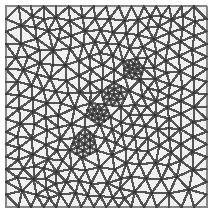
\includegraphics[width=\textwidth]{images/maxwell/maxwell_partition_inexact.pdf}
        \caption{Domain sequence $\domseq^{\mathrm{pinch}}$ with pinch}
        \label{fig:Maxwell_inexact_DoFmesh}
    \end{subfigure}
    \hfill
    \begin{subfigure}[b]{0.24\textwidth}
        \centering
        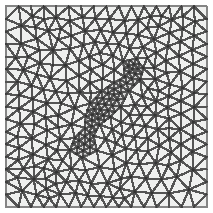
\includegraphics[width=\textwidth]{images/maxwell/maxwell_partition_exact.pdf}
        \caption{Admissible domain sequence  $\domseq^{\mathrm{padded}}$}
        \label{fig:Maxwell_exact_DoFmesh}
    \end{subfigure}
    \hfill
    \begin{subfigure}[b]{0.45\textwidth}
        \centering
        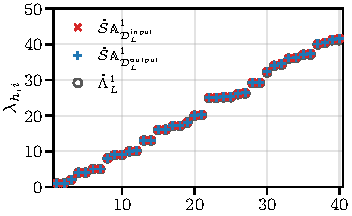
\includegraphics[width=\textwidth]{images/maxwell/maxwell_spectrum.pdf}
        \caption{Computed EVs over EV index}
        \label{fig:Maxwell_eigenvalues}
    \end{subfigure}
    \caption{Domain sequences and discrete spectra of the spaces $\hierSDFspaceZero{1}{\domseq^{\mathrm{pinch}}}{\L}$, $\hierSDFspaceZero{1}{\domseq^{\mathrm{padded}}}{\L}$ and $\FEECspaceZero{k}{\L}$.}
    \label{fig:maxwell_overview}
\end{figure}

%\FloatBarrier

\subsection{$1$-Form Laplace problem}
\label{subsec:vector_laplace}

% -----------------------------------------------------------------------
% NEW (2026-08-21): the problem statement, the assembly/solve material moved
% here from the Example at ex:matrix_assembly_old in Section~\ref{subsec:solve},
% and the error indicator now sit together in this subsubsection. The
% solution-snapshot figure moved down into "Approximation" with them.
% -----------------------------------------------------------------------
\subsubsection{Problem statement, discretisation, and solve}
\label{subsubsec:cl_problem}


The $1$-form Laplace problem is given by
\begin{equation}
    \label{eq:strong_laplace}
    (\extd \boldsymbol{\delta} + \boldsymbol{\delta} \extd) u = f
\end{equation}
on a domain $\M$. Since the operator $\boldsymbol{\delta}$ is not well-defined for a (subdivision) $1$-form, we introduce the auxiliary variable $\boldsymbol{\delta} \sigma = u$ and use the FEEC-typical mixed weak formulation: Find $\sigma \in H^1(\M)$ and $u \in \HcurlM{\M}$ such that
\begin{align}
    \label{eq:mixed_laplacian1}
    (\sigma, \tau)_\M - (u, \extd \tau)_\M &= 0 \qquad \forall \tau \in H^1(\M), \\
    \label{eq:mixed_laplacian2}
    (\extd \sigma, v)_\M + (\extd u, \extd v)_\M &= (f, v)_\M \qquad \forall v \in \HcurlM{\M}.
\end{align}

This section studies the circular layer test case from \cite{Cabanas.2026} to exercise the entire adaptive loop of \textsc{Solve}--\textsc{Estimate}--\textsc{Mark}--\textsc{Refine}--\textsc{Pad}. Its analytical solution is given by
\begin{equation}
    \label{eq:circular_layer_test_case}
    \Vec{u}_{\mathrm{CL}}(x) = \tanh \big(\alpha (\vvert{\vvert{x}}^2 - R^2) \big) \; \Vec{b}(x) \quad \text{with} \quad \Vec{b}(x) = \begin{bmatrix}
        2 x_2^2 (x_2 - 1)^2 (x_1^2 - x_1) (2 x_1 - 1) \\[2pt]
        2 x_1^2 (x_1 - 1)^2 (x_2^2 - x_2) (2 x_2 - 1)
    \end{bmatrix},
\end{equation}
where $\alpha = 100$, $R = 0.3$, and $\Vec{u}_{\mathrm{CL}}$ is the vector-proxy of the $1$-form $u_{\mathrm{CL}}$. The vector part $\Vec{b}(x)$ provides a background field while the $\tanh$ term adds a sharp, radially symmetric transition between $+\Vec{b}$ and $-\Vec{b}$ localised on the ring $\vvert{\vvert{x}} = R$. The right-hand side $f_{\mathrm{CL}}$ corresponding to $\Vec{u}_{\mathrm{CL}}$ can be computed using the (strong) Laplace equation~\eqref{eq:strong_laplace}. The problem carries no essential boundary conditions: both equations are natural in $\sigma$ and in $u$, so the discrete spaces are $\hierSDFspace{0}{\domseq}{\L}$ and $\hierSDFspace{1}{\domseq}{\L}$ rather than their vanishing-trace counterparts.

\guidance{The \textsc{Solve} step follows the pattern of Section~\ref{subsec:solve}. We use a standard finite element library like FEniCS~\citep{Logg.2012} to assemble the $0$-form mass matrix $\mathbf{M}_\L$ and the gradient-coupling matrix $\mathbf{B}_\L$ of Equation~\eqref{eq:mixed_laplacian1} and the curl--curl matrix $\mathbf{C}_\L$ of Equation~\eqref{eq:mixed_laplacian2} over the FEEC spaces $\FEECspace{k}{\L}$ on $\T_\L$, and never touch a subdivision basis function during assembly. Unrefining them with the adaptive subdivision $k$-form matrices $\Amat{k}{\activeDoFs}{\L}$ as in Equation~\eqref{eq:unrefinement} yields
\begin{equation}
    \label{eq:FE_matrix_assembly}
    \mathbf{M}_{\domseq} = (\Amat{0}{\activeDoFs}{\L})^\top \; \cdot \; \mathbf{M}_\L \; \cdot \; \Amat{0}{\activeDoFs}{\L},
    \quad
    \mathbf{C}_{\domseq} = (\Amat{1}{\activeDoFs}{\L})^\top \; \cdot \; \mathbf{C}_\L \; \cdot \; \Amat{1}{\activeDoFs}{\L},
    \quad
    \mathbf{B}_{\domseq} = (\Amat{0}{\activeDoFs}{\L})^\top \; \cdot \; \mathbf{B}_\L \; \cdot \; \Amat{1}{\activeDoFs}{\L}
\end{equation}
over the spaces $\hierSDFspace{k}{\domseq}{\L}$, together with the right-hand side $f_{\domseq} = (\Amat{1}{\activeDoFs}{\L})^\top \cdot f_\L$ of Equation~\eqref{eq:mixed_laplacian2}. The mixed problem assembles into the block system
\begin{equation}
    \label{eq:mixed_block_system}
    \begin{bmatrix}
        -\mathbf{M}_{\domseq} & \mathbf{B}_{\domseq} \\
        \mathbf{B}_{\domseq}^\top & \mathbf{C}_{\domseq}
    \end{bmatrix} \; \cdot \; \begin{bmatrix}
        \sigma_{\domseq} \\
        u_{\domseq}
    \end{bmatrix} = \begin{bmatrix}
        0 \\
        f_{\domseq}
    \end{bmatrix},
\end{equation}
whose matrix we denote by $K_{\domseq}$. It is symmetric indefinite, so we solve it with \emph{MINRES} and the block-diagonal SPD preconditioner
\begin{equation}
    \label{eq:preconditioner}
    \mathbf{P} =
    \begin{pmatrix}
        \mathbf{M}_{\domseq} & 0 \\
        0 & \mathbf{S_{\domseq}}
    \end{pmatrix},
    \qquad
    \mathbf{S}_{\domseq}= \mathbf{C}_{\domseq} + \mathbf{B}_{\domseq}^\top\, \mathrm{diag}(\mathbf{M}_{\domseq} \mathbf{1})^{-1}\, \mathbf{B}_{\domseq},
\end{equation}
in which $\mathbf{S}_{\domseq}$ approximates the Schur complement of the $(1,1)$ block by replacing $\mathbf{M}_{\domseq}^{-1}$ with a row-sum lumped inverse ($\mathbf{1}$ the all-ones vector of length $\vert \activeDoFSet{0}{} \vert$). A multilevel preconditioner, for instance BPX or a subdivision-aware multigrid V-cycle, would be the natural way to exploit the hierarchical structure of $\hierSDFspace{k}{\domseq}{\L}$, but constructing one for the subdivision basis is nontrivial, so we use the simpler level-agnostic choice above. Section~\ref{subsubsec:cl_performance} measures what that costs.}

\guidance{The \textsc{Estimate} step of Section~\ref{subsec:estimate} needs an indicator per face of the finest mesh $\T_\L$. We use the residual indicator that~\cite{Demlow.2014} derive for the mixed Hodge--Laplace problem on a general Hilbert complex. Their element indicator $\eta_0$ of Lemma~8, Equation~(4.6), collects the residual of the second equation~\eqref{eq:mixed_laplacian2}, their $\eta_{-1}$ of Lemma~7, Equation~(4.1), the residual of the first one~\eqref{eq:mixed_laplacian1}, and their Theorem~10, Equation~(4.18), proves the resulting estimator reliable, with the matching efficiency bounds in their Section~5. Specialising $\eta_0$ to $k=1$ in two dimensions, the harmonic contribution $p_h$ drops out because $\M$ is a topological disk, and $\boldsymbol{\delta} \extd u_h$ vanishes elementwise because $\extd (\iota u_h)$ is piecewise constant on $\T_\L$, where $\iota \colon \hierSDFspace{k}{\domseq}{\L} \hookrightarrow \FEECspace{k}{\L}$ is the inclusion into the fine FEEC space. What remains is the indicator
\begin{equation}
    \label{eq:cl_estimator}
    \eta^2_{\L,\fineIdxone} \; = \; h_{\face{\L}{\fineIdxone}}^2 \, \big\| f - \extd \sigma_h \big\|^2_{L^2(\face{\L}{\fineIdxone})}
    \; + \sum\limits_{\edge{\L}{\fineIdxtwo} \, \subset \, \partial \face{\L}{\fineIdxone}} h_{\edge{\L}{\fineIdxtwo}} \, \big\| [\![ \mathrm{curl} (\iota u_h) ]\!] \big\|^2_{L^2(\edge{\L}{\fineIdxtwo})},
\end{equation}
in which the first term is the elementwise residual of~\eqref{eq:mixed_laplacian2} and the second collects the curl--curl contribution through the jump $[\![ \cdot ]\!]$ of the piecewise constant $\mathrm{curl}(\iota u_h)$ across the interior edges of $\face{\L}{\fineIdxone}$. The indicator is evaluated on $\T_\L$ and aggregated to the faces of $\domseq$ by Equation~\eqref{eq:project_estimator_on_L_to_partition}, and from there to the vertices of $\domseq$ by Equation~\eqref{eq:vertex_residual}.}

\todo{\guidance{\textbf{Not paper text --- three points to settle about~\eqref{eq:cl_estimator}.}
\emph{(a)} It reproduces \texttt{weak\_forms/laplace/eta\_form\_Hcurl.ufl} exactly, which is what the runs of this section evaluate: \texttt{h**2*inner(f-grad(sigma),\,f-grad(sigma))*q*dx} plus \texttt{avg(h)*inner(jump(curl(u)),\,jump(curl(u)))*avg(q)*dS}. The superseded Example in Section~\ref{subsec:estimate} carried a third term $\|\sigma_h + \boldsymbol{\delta} u_h\|^2$ that the code never computes, so it was not moved across --- and its sign was wrong either way: \eqref{eq:mixed_laplacian1} gives $\sigma = \boldsymbol{\delta} u$, and Demlow--Hirani (4.1) reads $h_K \| \sigma_h - \boldsymbol{\delta} u_h \|_K$.
\emph{(b)} The $h_T^2$ and $h_e$ weights are confirmed: (4.1) and (4.6) weight element terms by $h_K$ and edge terms by $h_K^{1/2}$ before squaring. The \texttt{\textbackslash robert\{\}} marks on them can go.
\emph{(c)} \eqref{eq:cl_estimator} is a strict subset of the reliable estimator of Theorem~10. Not evaluated: all of $\eta_{-1}$, i.e.\ $h_K\|\sigma_h - \boldsymbol{\delta} u_h\|_K + h_K^{1/2} \| [\![ u_h \cdot n ]\!] \|_{\partial K}$; the two data terms $\| \boldsymbol{\delta} (f - \extd \sigma_h) \|_K$ and $\| [\![ (f - \extd \sigma_h) \cdot n ]\!] \|_{\partial K}$ of (4.6); and, since the problem has natural boundary conditions, the boundary-edge terms, which Demlow--Hirani read as the trace itself while the code sums interior edges only (\texttt{dS}).

\emph{Measured, $\L = 3$, three runs at identical settings:} adding the element term of $\eta_{-1}$, and adding its normal jump on top, reproduces the adaptive trajectory \emph{exactly} --- same faces, active DoFs, marked and padded faces, padding cycles, MINRES iterations and $L^2$ errors at every step, same stopping step --- while contributing between $0.04\%$ and $0.37\%$ of $\eta^2$. On a fixed uniform subdivision space represented on $\T_\L$ for growing $\L$, the share $\eta_{-1}/\eta_0$ falls monotonically with the number of subdivision steps, $0.39\%,\ 0.067\%,\ 0.042\%,\ 0.032\%$, so the omission gets safer as $\L$ grows.

\emph{The referee question this invites:} if the comparison was run, why not use the estimator with the proven properties? Only the data terms have a standard answer (data oscillation, higher order for the analytic $f$ of this test case, and flagged by Demlow--Hirani themselves as an artefact of the Hodge imbalance). Dropping $\eta_{-1}$ is a measurement, not an argument. Since the extra terms cost two DG0 form assemblies and no measurable time, the defensible choice is to make $\eta_0 + \eta_{-1}$ (boundary edges included, data terms out) the production estimator and re-run $\L = 3, 4, 5$; the $\L=3$ trajectory is already known to be unchanged.}}

\subsubsection{Approximation}

\begin{figure}[tb]
    \centering
    \begin{minipage}[c]{0.88\textwidth}
        \centering
        \begin{subfigure}[b]{0.33\linewidth}
            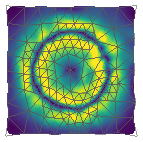
\includegraphics[width=\textwidth]{images/laplace_case/u_L4_step1.pdf}
            \caption{Step $1$.}
        \end{subfigure}\hfill
        \begin{subfigure}[b]{0.33\linewidth}
            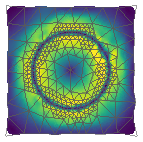
\includegraphics[width=\textwidth]{images/laplace_case/u_L4_step2.pdf}
            \caption{Step $2$.}
        \end{subfigure}\hfill
        \begin{subfigure}[b]{0.33\linewidth}
            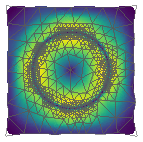
\includegraphics[width=\textwidth]{images/laplace_case/u_L4_step3.pdf}
            \caption{Step $3$.}
        \end{subfigure}
        \\[6pt]
        \begin{subfigure}[b]{0.33\linewidth}
            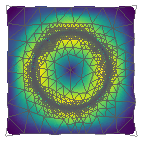
\includegraphics[width=\textwidth]{images/laplace_case/u_L4_step4.pdf}
            \caption{Step $4$.}
        \end{subfigure}\hfill
        \begin{subfigure}[b]{0.33\linewidth}
            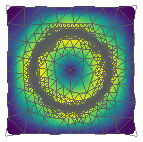
\includegraphics[width=\textwidth]{images/laplace_case/u_L4_step5.pdf}
            \caption{Step $5$.}
        \end{subfigure}\hfill
        \begin{subfigure}[b]{0.33\linewidth}
            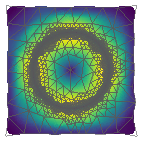
\includegraphics[width=\textwidth]{images/laplace_case/u_L4_step6.pdf}
            \caption{Step $6$.}
        \end{subfigure}
    \end{minipage}\hfill
    \begin{minipage}[c]{0.12\textwidth}
        \centering
        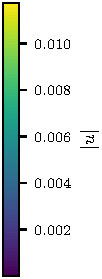
\includegraphics[trim = 0mm 0mm 5mm 0mm, clip, height=6.2cm]{images/laplace_case/u_colorbar_L4.pdf}
    \end{minipage}
    \caption{Snapshot of the adaptive solution $\vvert{\Vec{u}^n}$ after $n$ steps, approximated using $\hierSDFspace{k}{\domseq}{4}$ with $\L = 4$, overlaid with the admissible domain sequence $\domseq^n$ as a grey wireframe. The colorbar represents the magnitude $\vvert{\Vec{u}^6}$ after step $6$ and is applied across all steps.}
    \label{fig:adaptive_solution}
\end{figure}

\smallskip

\newcommand{\laststep}{{\mathrm{N}_\L}}

Figure~\ref{fig:adaptive_solution} displays the solution's vector proxy $\Vec{u}^n$ after $n$ steps of the adaptive loop with Do\"rfler parameter $\theta = 0.9$ and $\L=4$, meaning that the domain sequence cannot be refined beyond that level. The refinement stays concentrated around the circle to capture the sharp transition of the analytical solution. We denote the domain sequences across the steps by $\domseq^n$ and the final step of the adaptive loop by $\laststep$.

The marking is driven by the vertex-based estimator $\nu^2_\coarseIdxtwo$ from Equation~\eqref{eq:vertex_residual}. Figure~\ref{fig:cl_convergence} shows how this marking drives the $L^2$ error
\begin{equation}
    \label{def:L2_error}
    \Ltwoerror^n \coloneq \vert\vert \vec{u}^n - \Vec{u}_{\mathrm{CL}} \vert\vert_{L^2(\T_\L)}
\end{equation}
computed against the analytical solution $\Vec{u}_{\mathrm{CL}}$ for $\L \in \{3, 4, 5\}$. We omit the superscript $n$ whenever it does not matter or we address the error of a reference solution using $\FEECspace{1}{\L}$.

The left panel~\ref{fig:cl_saturation_fig} compares the total estimator $\eta$ and the refinable estimator $\rho$ from Equation~\eqref{def:total_and_refinable_residuals}. For the first few levels, the two coincide. The two estimators diverge as soon as the partition $\domseq^n$ contains faces on the finest level $\L$ because the residuals of these faces are not included in the refinable estimator. The total estimator stagnates at a non-zero value that depends on $\L$, whereas the refinable estimator converges towards $0$ as the partition $\domseq^n$ transitions towards $\T_\L$. The simulation in Figure~\ref{fig:adaptive_solution} used exactly that behaviour as stopping criterion, terminating the simulation as soon as the saturation rate $\xi = \rho^2 / \eta^2$ from Equation~\eqref{eq:saturation_rate} satisfies $\xi \leq 0.05$.

Figure~\ref{fig:cl_l2_vs_dofs} reports the errors $\Ltwoerror^n$ depending on the number of active $1$-form DoFs $\vvert{\activeDoFSet{1}{}(\domseq^n)}$. Note that the figure also include the FEEC references $\FEECspace{1}{\L}$ (hollow squares). The errors of the adaptive method converge quickly in the first steps but as the estimators diverge from each other, the $L^2$ errors $\Ltwoerror^n$ start to plateau. We consider that plateau to be the converged state of the adaptive solver. Figure~\ref{fig:cl_l2_vs_dofs} and Table~\ref{tab:cl_headline} confirm that the converged adaptive solution with $\xi \leq 0.05$ has $3.3$, $4.6$ and $5.9$ times less $1$-form DoFs than the reference solutions of $\FEECspace{1}{\L}$ for $\L=3$, $4$ and $5$, respectively. Loosening the stopping criterion to $\xi\leq 0.3$ increases the DoF saving to $3.7$, $5.4$ and $9.3$, cf. Table~\ref{tab:cl_headline}.

% Independently adjustable panel widths: panel (a) lost its y-axis label, which
% shrinks its tight-cropped bounding box relative to panel (b), so the two may
% need slightly different \textwidth fractions to come out the same height.
\newcommand{\clSatWidth}{0.49\textwidth}
\newcommand{\clLtwoWidth}{0.49\textwidth}
\begin{figure}[tb]
    \centering
    \begin{subfigure}[t]{\clSatWidth}
        \centering
        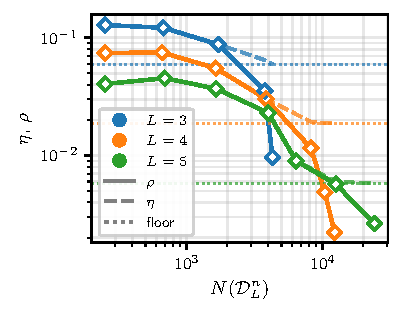
\includegraphics[width=\textwidth]{images/laplace_case/fig_estimator_saturation.pdf}
        \caption{Total and refinable estimators over the number $\vvert{\activeDoFSet{1}{}(\domseq^n)}$ of active $1$-form DoFs}
        \label{fig:cl_saturation_fig}
    \end{subfigure}\hfill
    \begin{subfigure}[t]{\clLtwoWidth}
        \centering
        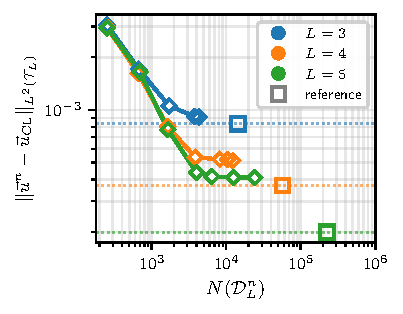
\includegraphics[width=\textwidth]{images/laplace_case/fig_l2_vs_dofs.pdf}
        \caption{$L^2$ error over the number $\vvert{\activeDoFSet{1}{}(\domseq^n)}$ of active $1$-form DoFs}
        \label{fig:cl_l2_vs_dofs}
    \end{subfigure}
    \caption{Panel (a) displays the total estimator $\eta$ and the refineable estimator $\rho$ against the number $\vert \activeDoFSet{1}{} \vert$ of active $1$-form DoFs for $\L \in \{3, 4, 5\}$. Every hollow diamond marks a step. Together, these estimators drive and eventually terminate the adaptive loop. Panel (b) shows the true $L^2$ error against $\vert \activeDoFSet{1}{} \vert$ for the adaptive methods (solid lines with hollow diamonds to mark steps) and FEEC references $\FEECspace{1}{\L}$ (hollow squares) for $\L \in \{3, 4, 5\}$.}
    \label{fig:cl_convergence}
\end{figure}

\begin{table}[tb]
    \centering
    \small
    \begin{tabular}{@{}r cc@{\hspace{14pt}} cccc@{\hspace{14pt}} cccc@{}}
        \toprule
        & \multicolumn{2}{c}{FEEC reference $\FEECspace{1}{\L}$} & \multicolumn{4}{c}{adaptive, $\xi \leq 0.05$} & \multicolumn{4}{c}{adaptive, $\xi \leq 0.3$} \\
        \cmidrule(lr){2-3}\cmidrule(lr){4-7}\cmidrule(lr){8-11}
        \multirow{2}{*}{$L$} & \multirow{2}{*}{$\vert \activeDoFSet{1}{} \vert$} & $\Ltwoerror$ & \multirow{2}{*}{$\vert \activeDoFSet{1}{} \vert$} & $\Ltwoerror$ & DoF & $L^2$ & \multirow{2}{*}{$\vert \activeDoFSet{1}{} \vert$} & $\Ltwoerror$ & DoF & $L^2$ \\
        & & $(\cdot 10^{-4})$ & & $(\cdot 10^{-4})$ & saving & gap & & $(\cdot 10^{-4})$ & saving & gap \\
        \midrule
        3 & $10\,688$  & $8.34$ & $3\,265$  & $9.09$ & $\mathbf{3.3\times}$ & $1.09\times$ & $2\,869$  & $9.18$ & $\mathbf{3.7\times}$ & $1.10\times$ \\
        4 & $42\,496$  & $3.70$ & $9\,235$  & $5.13$ & $\mathbf{4.6\times}$ & $1.39\times$ & $7\,874$  & $5.21$ & $\mathbf{5.4\times}$ & $1.41\times$ \\
        5 & $169\,472$ & $2.00$ & $28\,588$ & $4.06$ & $\mathbf{5.9\times}$ & $2.03\times$ & $18\,280$ & $4.10$ & $\mathbf{9.3\times}$ & $2.06\times$ \\
        \bottomrule
    \end{tabular}
    \caption{Comparison of the adaptive method, terminated at the headline tolerance $\xi \leq 0.05$ and at the looser $\xi \leq 0.3$, against the FEEC reference $\FEECspace{1}{\L}$, for $\L \in \{3, 4, 5\}$. All $\Ltwoerror$ values are in units of $10^{-4}$. \emph{DoF saving} is the ratio of DoFs of the reference to the adaptive method, and the \emph{$L^2$ gap} is the ratio of the respective $\Ltwoerror$ for both methods. Loosening the stopping criterion from $\xi \leq 0.05$ to $\xi \leq 0.3$ trades a small increase in $L^2$ gap for a substantially larger DoF saving at every $\L$.}
    \label{tab:cl_headline}
\end{table}

\newcommand{\Ltwogap}{g}
Notably, Figure~\ref{fig:cl_l2_vs_dofs} shows that the converged $L^2$ error $\Ltwoerror^\laststep(\hierSDFspace{1}{\domseq}{\L})$ of the adaptive method does not coincide with the reference $L^2$ error $\Ltwoerror(\FEECspace{1}{\L})$. Table~\ref{tab:cl_headline} compares the final states of the adaptive method terminated at $\xi \leq 0.05$ and $\xi \leq 0.3$ with the FEEC reference. The tabulated $L^2$ errors allow us to compute the \emph{$L^2$ gap} $\Ltwogap(\L)$ by
\begin{equation}
    \Ltwogap(\L) \coloneq \Ltwoerror^\laststep(\hierSDFspace{1}{\domseq}{\L}) \; / \; \Ltwoerror(\FEECspace{1}{\L}).
\end{equation}
Table~\ref{tab:cl_headline} reveals that, as $\L$ and thus the DoF saving factor increase, so does the $L^2$ gap of the approximation errors. This is not a solver defect, but the price of saving DoFs. Marking in the energy norm concentrates refinement on the sharp $\tanh$ ring, where the residual is large, and leaves the smooth bulk coarse.

We verify this directly for $L=4$ by integrating $\vvert{u_h-u}^2$ against a sharp indicator function of width $w=0.05$ tracking the transition circle to obtain the ring error $r$. Integrating against the indicator's nodal complement in $\CG_1$ yields to the bulk error $b$. The two contributions add up exactly to the total $L^2$ error so that $\Ltwoerror^2 = r^2 + b^2$, for both the adaptive solution and the FEEC reference at the same $\L$. For $\L=4$, we measured
\begin{equation}
\begin{alignedat}{4}
    &r(\hierSDFspace{1}{\domseq}{4}) &&= 3.30\cdot10^{-4} \, , \qquad &&b(\hierSDFspace{1}{\domseq}{4}) &&= 3.93\cdot10^{-4} \, ,\\
    &r(\FEECspace{1}{4}) &&= 3.30\cdot10^{-4} \,, \qquad &&b(\FEECspace{1}{4}) &&= 1.69\cdot10^{-4}.
\end{alignedat}
\end{equation}
The ring error agrees closely between the two methods (differing by only $0.02\%$), while the bulk error differs substantially. This implies that the $L^2$ gap is a function of the bulk errors growing apart between the two methods, not an artifact of the ring. In this sense, the $L^2$ gap explicitly measures the loss of accuracy incurred by saving DoFs. Where that unavoidable gap concentrates is a choice, not a necessity. This is where reading the adaptive loop backwards, as \emph{greedy coarsening} of the fine reference space rather than incremental refinement of a coarse one, is useful: Dörfler marking greedily decides, step by step, which part of the fine space to keep active, based on the residual estimator. Because the sharp $\tanh$ ring dominates that estimator, coarsening is cheapest in estimator terms everywhere except the ring, so the bulk is coarsened away first and absorbs almost all of the $L^2$ gap.

\subsubsection{Performance metrics}
\label{subsubsec:cl_performance}

This section explores two metrics: the overhead of interface DoFs and additional DoFs due to padding, and the wallclock time of the adaptive loop.

Table~\ref{tab:padding_interface_L4} tracks the number of active DoFs and how they split into patch versus interface and marked versus padded for the simulation with $\L=4$. First, the table shows that the fraction of active $1$-form interface DoFs is between $20\%$ and $30\%$ of the overall DoF count. Since the underlying geometry is a thin annulus, this is already a pessimistic estimate. Nevertheless, the interface DoFs never dominate the patch DoFs. Second, padding never exceeds $22$ faces (step $5$), under $8\%$ of the $279$ marked faces of that step. This implies that neither the interface DoFs nor the padding constitute the bulk of the overall active DoFs.

\begin{table}[tb]
  \centering
  \begin{tabular}{r@{\hspace{40pt}}r@{\hspace{16pt}}rrr@{\hspace{40pt}}rrr@{\hspace{16pt}}r}
    \toprule
    \multirow{2}{*}{step} & \multirow{2}{*}{$\vert \activeDoFSet{1}{} \vert$} & \multicolumn{3}{c}{splits into} & \multirow{2}{*}{$\vert \F(\domseq) \vert$} & \multicolumn{2}{c}{of which refined} & \multirow{2}{*}{\guidance{$q$}} \\
    \cmidrule(r{40pt}){3-5}\cmidrule(lr){7-8}
    & & patch & interface & fraction & & marked & padded & \\
    \midrule
    0 & 181  & 181  & 0    & $0\%$  & 110  & 38  & 0  & \guidance{0} \\
    1 & 495  & 390  & 105  & $21\%$ & 328  & 94  & 4  & \guidance{1} \\
    2 & 1245 & 897  & 348  & $28\%$ & 847  & 229 & 9  & \guidance{1} \\
    3 & 2936 & 2112 & 824  & $28\%$ & 2016 & 452 & 12 & \guidance{1} \\
    4 & 6260 & 4545 & 1715 & $27\%$ & 4314 & 314 & 9  & \guidance{1} \\
    5 & 7874 & 6035 & 1839 & $23\%$ & 5385 & 279 & 22 & \guidance{1} \\
    6 & 9235 & 7335 & 1900 & $21\%$ & 6293 & ---   & ---  & \guidance{---} \\
    \bottomrule
  \end{tabular}
  \caption{Metrics for all steps of the adaptive loop with $\L=4$. The first half shows the $1$-form DoFs and how they split into patch and interface DoFs, alongside the fraction of overall DoFs that are interface DoFs. The second half reports the number of faces of the admissible domain sequence $\domseq$ at the end of the step, and how they split into marked faces based on the estimator and additional refinement due to padding. \guidance{The last column reports the number $q$ of productive \textsc{Pad} passes of Section~\ref{subsec:termination} in that step, which is zero exactly when no predicate fired and never exceeds one anywhere in the run.}}
  \label{tab:padding_interface_L4}
\end{table}

\smallskip

The most relevant shortcoming of methods the adaptive subdivision $k$-form spaces is that saving DoFs does not translate to faster solves. Table~\ref{tab:solve_stats_L4} summarises the important metrics around the solve, including the wallclock time needed by the MINRES solver alongside the DoF count, the number of iterations, the condition number of the preconditioned system matrix $P^{-1}K_{\domseq^n}$, and the number of non-zero elements of $K_{\domseq^n}$ per DoF. Finally, we list the metrics for the fine FEEC reference $\FEECspace{k}{\L}$ with $\L=4$.

The wallclock times reveal that the solver performance degrades rapidly as the adaptive iterations increase. In fact, the FEEC reference method is about $130$ times faster than the adaptive solve of step $6$ even though it has roughly $4.7$ times as many DoFs. The reasons for that are found in the last three columns of Table~\ref{tab:solve_stats_L4}. First, the number of iterations needed for the MINRES solver to converge skyrocket initially until they start to become flat around step $4$. This happens due to the successive activation of basis functions across finer and finer levels, until at step $4$ the finest possible basis functions are first included in the adaptive space. This means that the condition number $\kappa(P^{-1}K_{\domseq^n})$ increases until then, explaining the increased number of iterations. This is a conditioning effect distinct from the rank-deficiency discussed in Section~\ref{subsec:unrefinement_and_solve}. $\domseq^n$ remains a admissible domain sequence throughout the loop, so $\Amat{k}{\activeDoFs}{\L}$ has full column rank at every step, yet $\kappa(P^{-1}K_{\domseq^n})$ still grows. The second reason for the large wallclock times is that the increased number of nonzero entries $\text{nnz}(K_{\domseq^n})/(\vert \activeDoFSet{0}{} \vert + \vert \activeDoFSet{1}{} \vert)$ per active DoF increases the number of operations per MINRES iteration. The increase of non-zero entries is due to the smoothing nature of subdivision, meaning that coarse basis functions have larger supports and thus cover a lot of triangles of $\T_\L$. The unrefinement step in Equation~\ref{eq:FE_matrix_assembly} extends this large number of non-zeros to $K_{\domseq}$.

\smallskip

The adaptive method thus only wins in DoFs and memory, not wall-clock, with the current solver. A truncated basis in the spirit of THB-splines \citep{Gianelli.2016} might be able to mitigate that problem. Truncating each coarse active basis function's representation over the region already covered by finer active DoFs would remove exactly the redundant coarse/fine support overlap responsible for the ill-conditioning and reduces the number of non-zeros, both without changing the discrete space itself. This means we would target both measured mechanisms directly, rather than working around them with a different solver. Truncating the subdivision-induced basis functions will be a subject of future work.

\begin{table}[tb]
  \centering
  \begin{tabular}{r@{\hspace{16pt}}r@{\hspace{16pt}}r@{\hspace{16pt}}r@{\hspace{16pt}}r@{\hspace{16pt}}r}
    \toprule
    \multirow{2}{*}{step} & wallclock & DoF count & \multirow{2}{*}{iterations} & \multirow{2}{*}{$\kappa(P^{-1}K_{\domseq})$} & \multirow{2}{*}{$\dfrac{\mathrm{nnz}(K_{\domseq})}{\vert \activeDoFSet{0}{} \vert + \vert \activeDoFSet{1}{} \vert}$} \\
     & time & $\vert \activeDoFSet{0}{} \vert + \vert \activeDoFSet{1}{} \vert$ & & & \\
    \midrule
    0 & $0.06\,\mathrm{s}$    & 253  & 63  & 9.98  & 77.7  \\
    1 & $1.57\,\mathrm{s}$    & 663  & 241 & 82.7  & 129.6 \\
    2 & $18.4\,\mathrm{s}$    & 1\,644  & 474 & 107.7 & 177.8 \\
    3 & $125.1\,\mathrm{s}$   & 3\,857  & 606 & 112.8 & 156.5 \\
    4 & $602.5\,\mathrm{s}$   & 8\,207  & 656 & 111.4 & 126.1 \\
    5 & $974.0\,\mathrm{s}$   & 10\,364  & 672 & 111.6 & 116.0 \\
    6 & $1380.9\,\mathrm{s}$  & 12\,178  & 692 & 103.2 & 106.2 \\
    \midrule
    FEEC reference $\FEECspace{k}{\L}$ & $10.6\,\mathrm{s}$   & $56\,833$ & 25  & 4.11  & 11.4  \\
    \bottomrule
  \end{tabular}
  \caption{Solve metrics for all steps of the adaptive simulation with $\L=4$. The fine superspace $\FEECspace{k}{4}$ is included as a reference. $\kappa(P^{-1}K_{\domseq})$ is the estimated condition number of the preconditioned operator after unrefinement, see Equation~\ref{eq:FE_matrix_assembly} and the preconditioner $\mathbf{P}$ defined in Equation~\ref{eq:preconditioner} (\S~\ref{subsec:solve}). The term \emph{nnz} refers to the number of non-zero elements of a matrix, and to obtain $\mathrm{nnz}(K_{\domseq})/(\vert \activeDoFSet{0}{} \vert + \vert \activeDoFSet{1}{} \vert)$ we normalised by the number of active DoFs.}
  \label{tab:solve_stats_L4}
\end{table}

\section{Conclusion}

\robert{We have presented a complete matrix-level framework for hierarchical subdivision $k$-form spaces and their use in an adaptive loop for structure-preserving PDE discretisations. The central observation is that any active subdivision basis function is a column of an accumulated subdivision matrix $\Smat{k}{\l}{\L}$; selecting columns according to a admissible domain sequence produces a hierarchical space $\hierSDFspace{k}{\domseq}{\L}$ whose linear independence and de Rham exactness are guaranteed by the partition condition proved in the companion paper~\cite{companion_paper}. Once the hierarchical subdivision matrix $\Amat{k}{\activeDoFs}{\L}$ is assembled, all bilinear forms are obtained by Galerkin restriction of the embedding-level operators without recomputing any integrals, and the active-space linear system reduces to standard sparse linear algebra on the finest mesh $\T_\L$.

The adaptive loop adds a subdivision-specific \textsc{Pad} step to the standard \textsc{Solve}--\textsc{Estimate}--\textsc{Mark}--\textsc{Refine} cycle. Padding alternates pinch resolution with \checkit{confinement padding} and grading to a fixed point: pinch resolution repairs a pinched coarse region that would otherwise carry a spurious harmonic (a closed but non-exact discrete $1$-form, breaking de Rham exactness), while \checkit{confinement padding} and grading enforce the interior-vertex (Good-vertex) requirement and bound the level jump at coarse/fine interfaces. \guidance{All three rules} only ever refine, are local, and are inexpensive relative to the linear solve\guidance{, and the iteration reaches a fixed point after finitely many passes (Section~\ref{subsec:termination})}.

The numerical experiments confirm the two key structural properties of the framework. For the Maxwell eigenvalue problem, exact admissible domain sequences reproduce the reference FEEC spectrum without spurious modes; inexact ones introduce them. This serves as a direct diagnostic for the correctness of the active-DoF construction and the de Rham complex structure. For the mixed vector Laplace equation, the adaptive loop concentrates refinement at the location of steep gradients and achieves convergence behaviour consistent with the hierarchical approximation theory.

Several directions remain open. \guidance{The most immediate is internal to the framework: Problem~\ref{prob:padding_passes} asks for a bound on the number of productive \textsc{Pad} passes in terms of the control mesh alone. Section~\ref{subsec:termination} isolates the two mechanisms a padding operator would have to break to admit one, which makes them concrete targets for a redesigned \textsc{Pad}.} The precise correspondence between the subdivision PAD step and the $L$-chain completion used in hierarchical B-spline AFEM~\cite{Cabanas.2026} has not been established; clarifying this connection would relate the two frameworks and potentially enable convergence proofs to be transferred. On the solver side, the block-diagonal LDLT preconditioner used here is effective for the problem sizes considered, but a multigrid preconditioner that respects the larger-than-Whitney supports of the subdivision basis would reduce the per-step cost for larger problems; this requires a prolongation operator compatible with $\Amat{k}{\activeDoFs}{\L}$ and is left for future work. Finally, a promising direction is to adopt the overlapping patch framework of Bressan~\cite{Bressan.2024} in place of the non-overlapping admissible domain sequence used here. Overlapping patches can provide a richer set of admissible active-DoF configurations and may admit a more flexible PAD step, at the cost of requiring a partition-of-unity treatment to maintain linear independence; adapting the matrix-level assembly and the de Rham complex to that setting is an open problem.}

\bibliography{references}

\appendix

\section{Active-DoF assembly pseudo-code}
\label{app:active_dof_pseudocode}

This appendix gives the full active-DoF assembly routine
$\textsc{BuildActiveDoFs}$. It evaluates
Definition~\ref{def:active_k_form_dofs} directly, one level at a time. Each level needs three
sets and no state carried from any other level: the region $\M_\l$, its extension
$\extendedPatch{\M}_\l$, and the ancestor patch $\ancestorPatch{\M_{\l+1}}$ of the next finer
region. The selection $\mathring{\K}^k_\l(\cdot)$ is the membership test of
Definition~\ref{def:open_patch_dofs}: a simplex qualifies exactly when every level-$\l$ face
containing it lies in the region, which is a single pass over the face-incidence relation.

The regions themselves are recovered downward from the leaf partition, using that
quadrisection assigns each level-$(\l\!+\!1)$ face the parent it was split from. Because the
levels are independent, the loop below may be run in any order, or in parallel.

\begin{algorithm}[H]
\caption{$\textsc{BuildActiveDoFs}(\domseq[\L])$: active degrees of freedom from a domain sequence}
\label{alg:buildactivedofs}
\BlankLine
\KwIn{domain sequence $\domseq[\L]$ given by its leaf partition, form degree $k$}
\KwOut{active DoFs $\activeDoFSet{k}{}(\domseq[\L])$, tagged by level}
\BlankLine
\tcp{1.\ Recover the regions downward from the leaf partition}
$\M_\L \leftarrow$ leaf faces at level $\L$\;
\For{$\l = \L - 1, \, \ldots, \, \lzero$}{
    $\M_\l \leftarrow \{\, \mathrm{parent}(f) \; : \; f \in \M_{\l+1} \,\} \; \guidance{\sqcup} \;$ leaf faces at level $\l$\;
}
\BlankLine
\tcp{2.\ One independent set difference per level}
$\activeDoFSet{k}{} \leftarrow \emptyset$\;
\For{$\l = \lzero, \, \ldots, \, \L$}{
    \tcp{(a) extension: every level-$\l$ face carrying a vertex of $\M_\l$}
    $\extendedPatch{\M}_\l \leftarrow \bigcup_{\vertex{\l}{\coarseIdxone} \in \V_\l(\M_\l)} \FVl{\l}(\vertex{\l}{\coarseIdxone})$\;
    \tcp{(b) removed region: the level-$\l$ faces refined beyond $\l$}
    $A_\l \leftarrow \ancestorPatch{\M_{\l+1}}$ \quad \tcp*{$A_\L = \emptyset$ by convention}
    \tcp{(c) select by Definition~\ref{def:open_patch_dofs}: all containing faces inside}
    $I_\l \leftarrow \{ \simplex{k}{\l}{\coarseIdxone} \; : \; \F\K^k_\l(\simplex{k}{\l}{\coarseIdxone}) \subseteq \extendedPatch{\M}_\l \}$\;
    $R_\l \leftarrow \{ \simplex{k}{\l}{\coarseIdxone} \; : \; \F\K^k_\l(\simplex{k}{\l}{\coarseIdxone}) \subseteq A_\l \}$\;
    $\activeDoFSet{k}{} \leftarrow \activeDoFSet{k}{} \; \guidance{\sqcup} \; \big( I_\l \setminus R_\l \big)$\;
}
\Return $\activeDoFSet{k}{}$\;
\end{algorithm}

\end{document}